\section*{\underline{Aufgabe 17}}

\subsection*{a)}

%vom Inhalt d passt 1 besser im Text steht 2
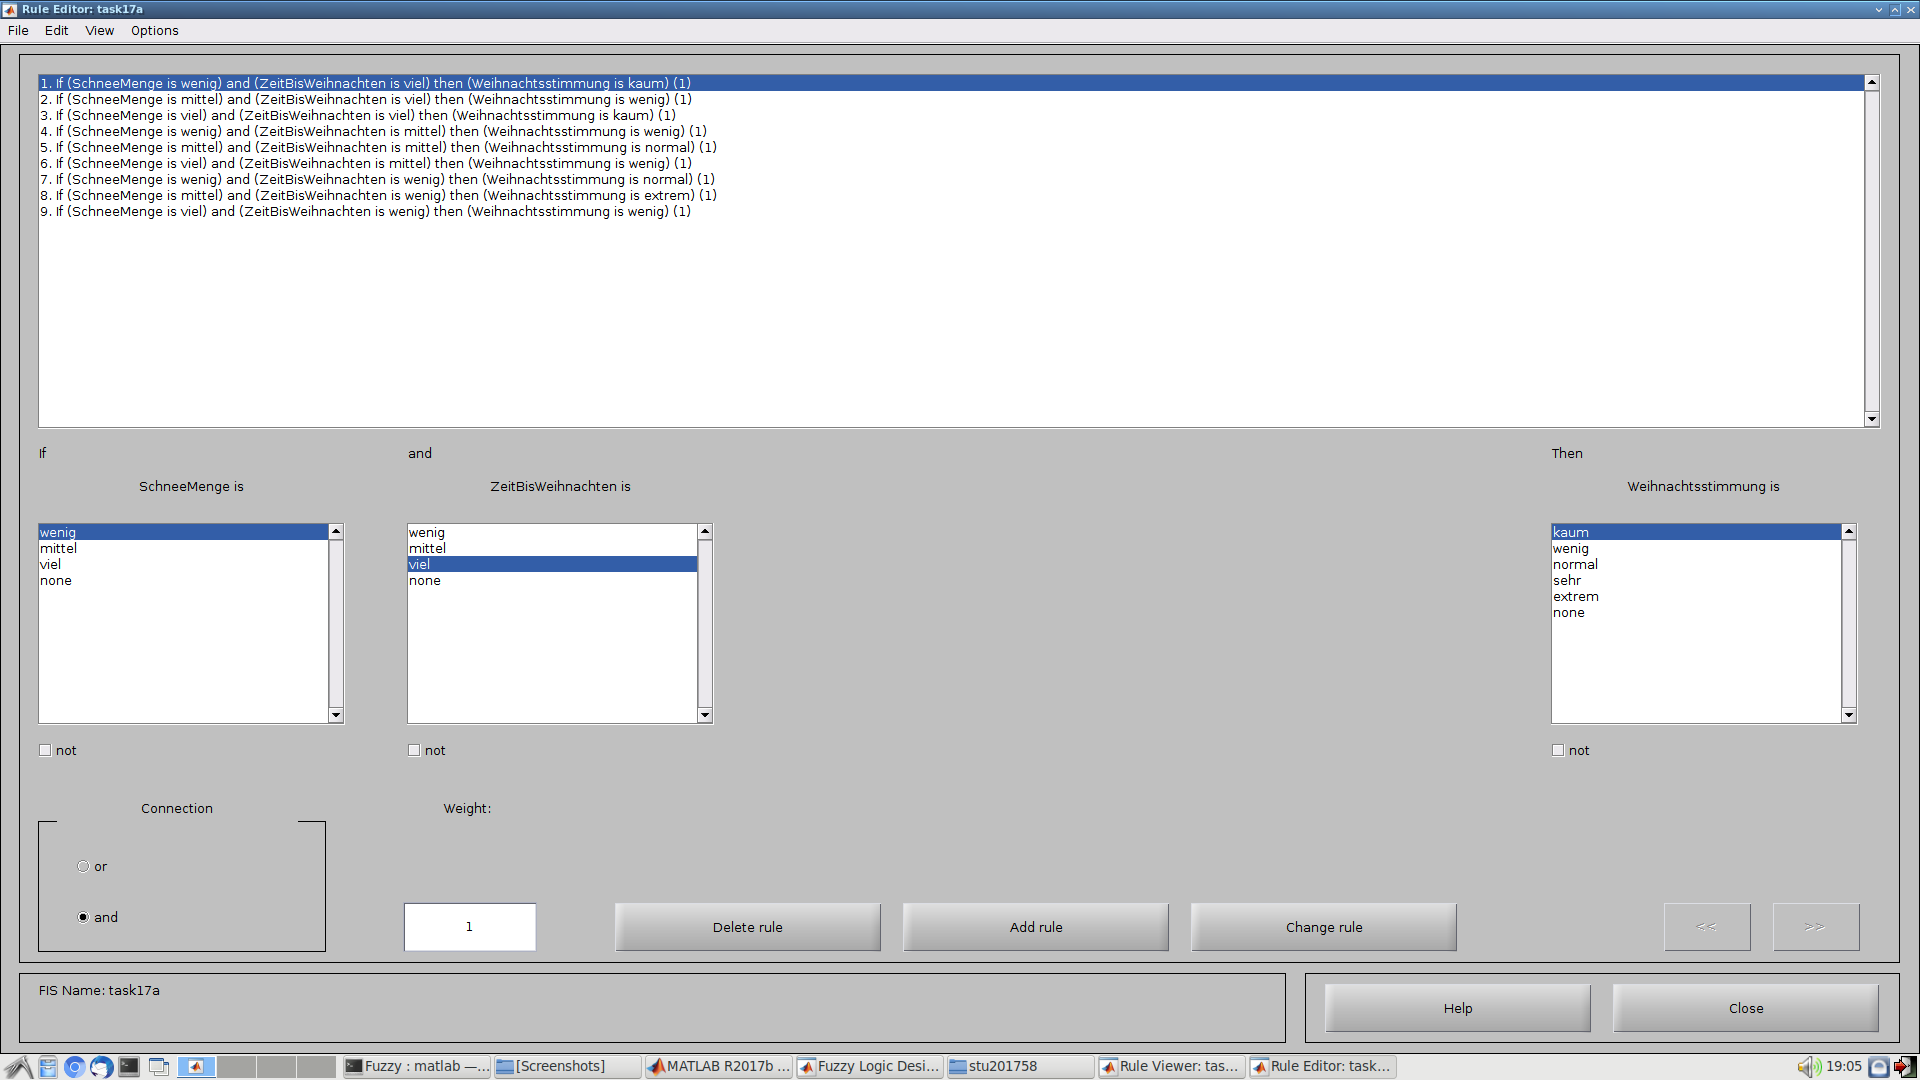
\includegraphics[width=\textwidth]{part/screenshots/fuzzy-17a-1}
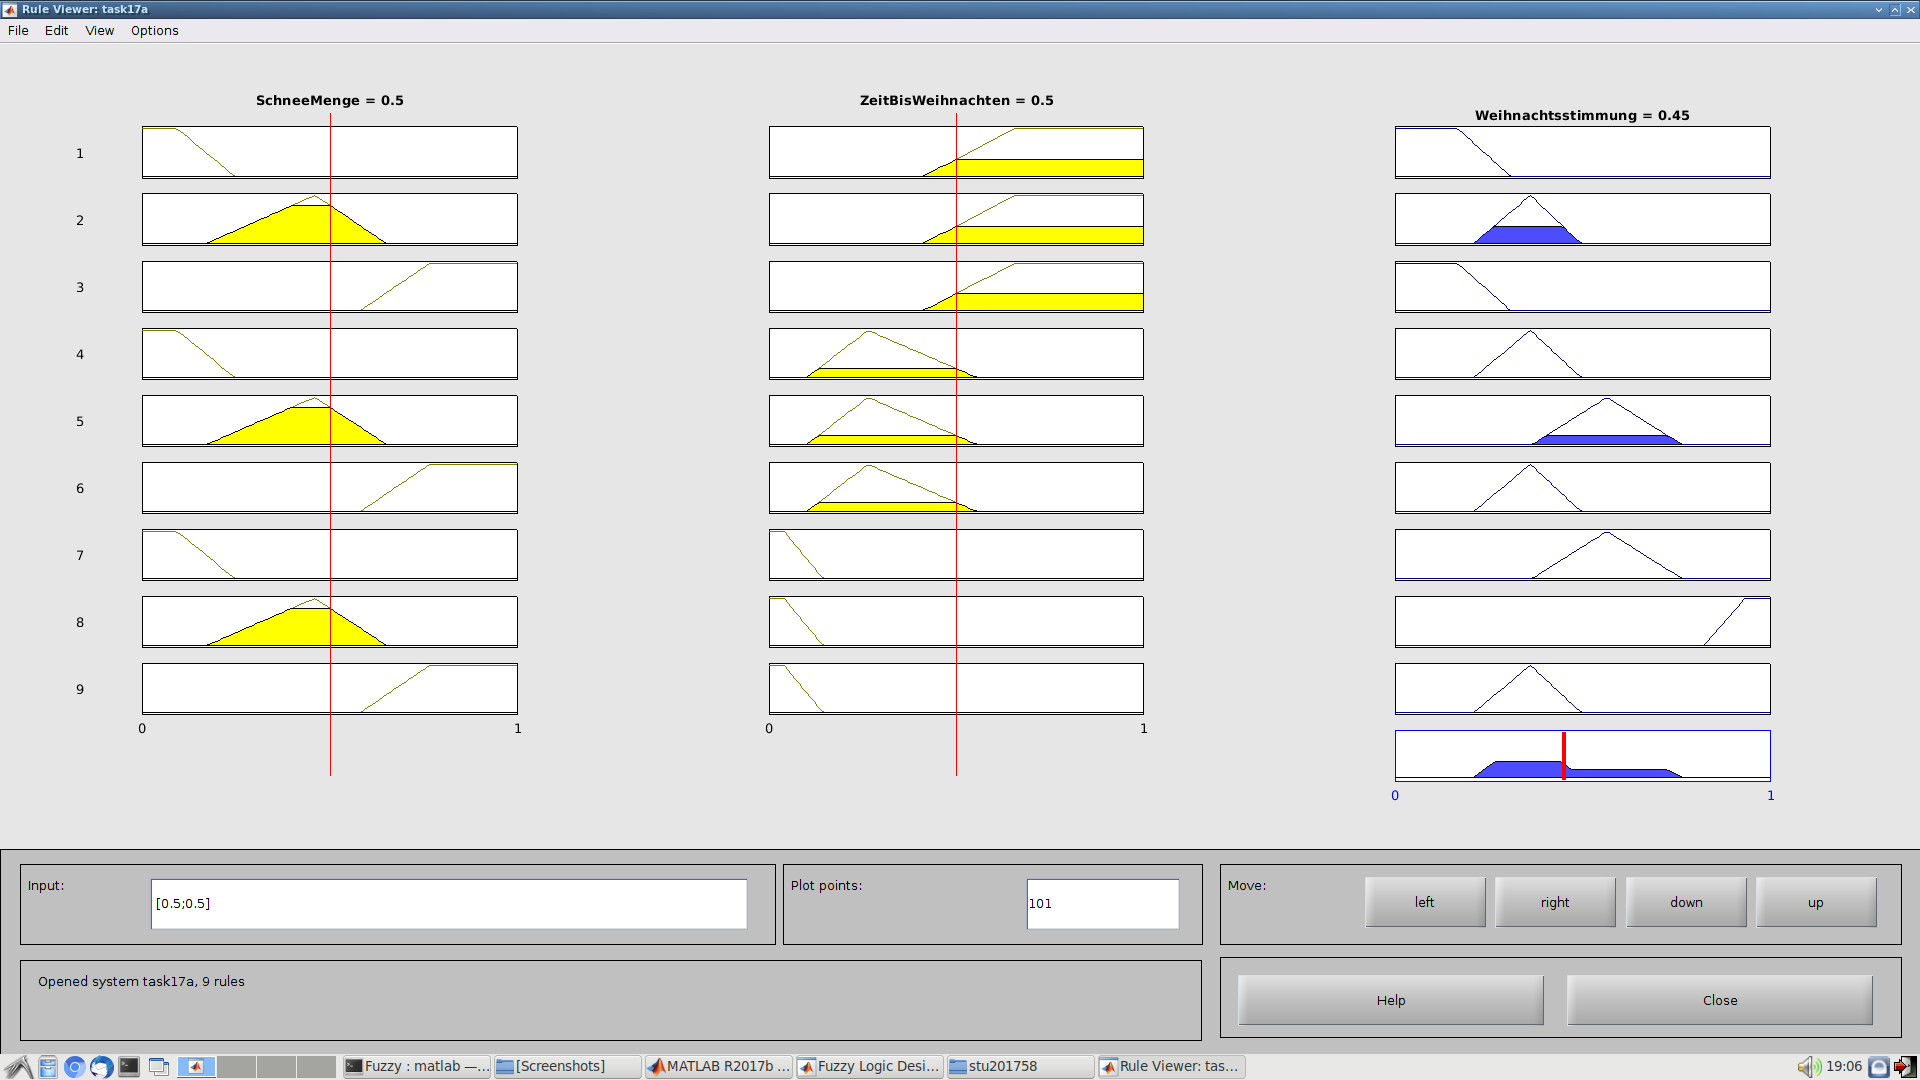
\includegraphics[width=\textwidth]{part/screenshots/fuzzy-17a-2}

\subsection*{b)}
%TODO man sollte vielleicht bespiele nehmen wo mehr als 1 MF zutrifft
%dann müssen auch die vergleiche in c) und d) angepasst werden

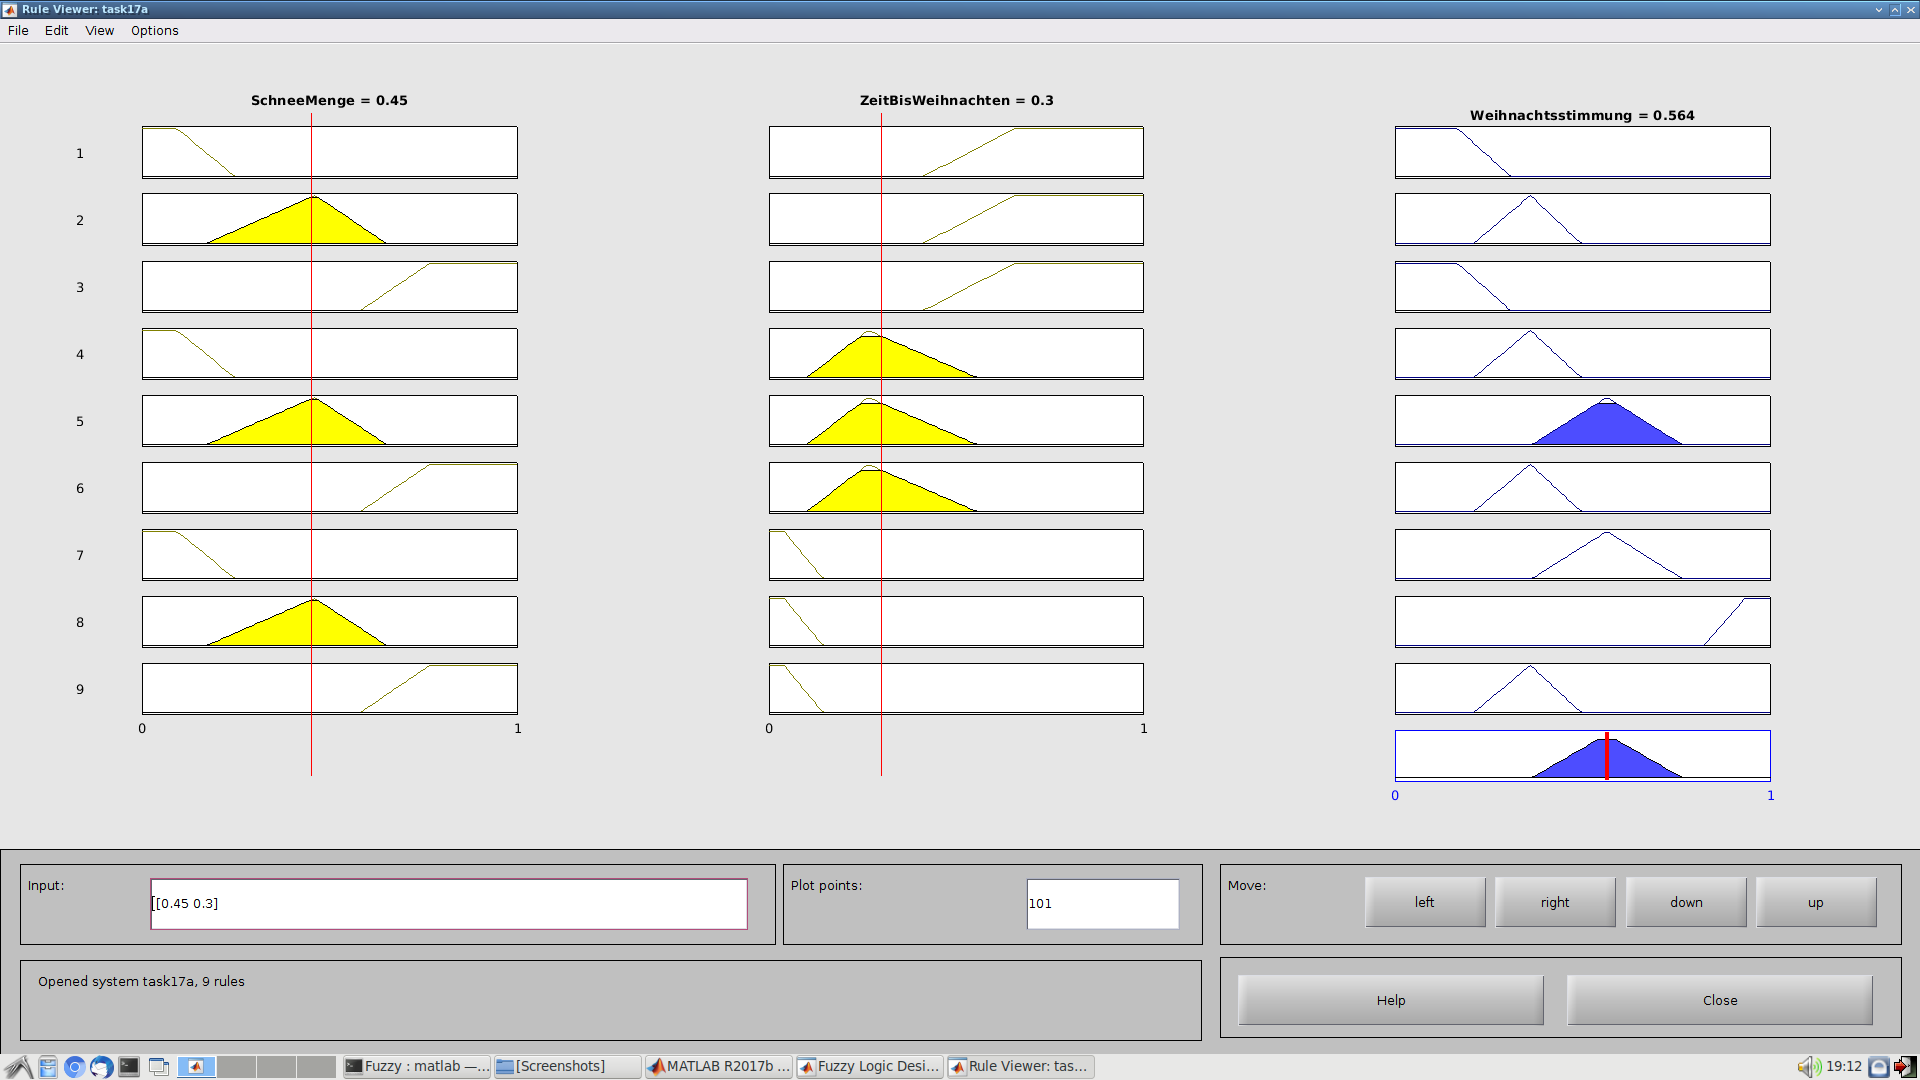
\includegraphics[width=\textwidth]{part/screenshots/fuzzy-17b-0,45-0,3}
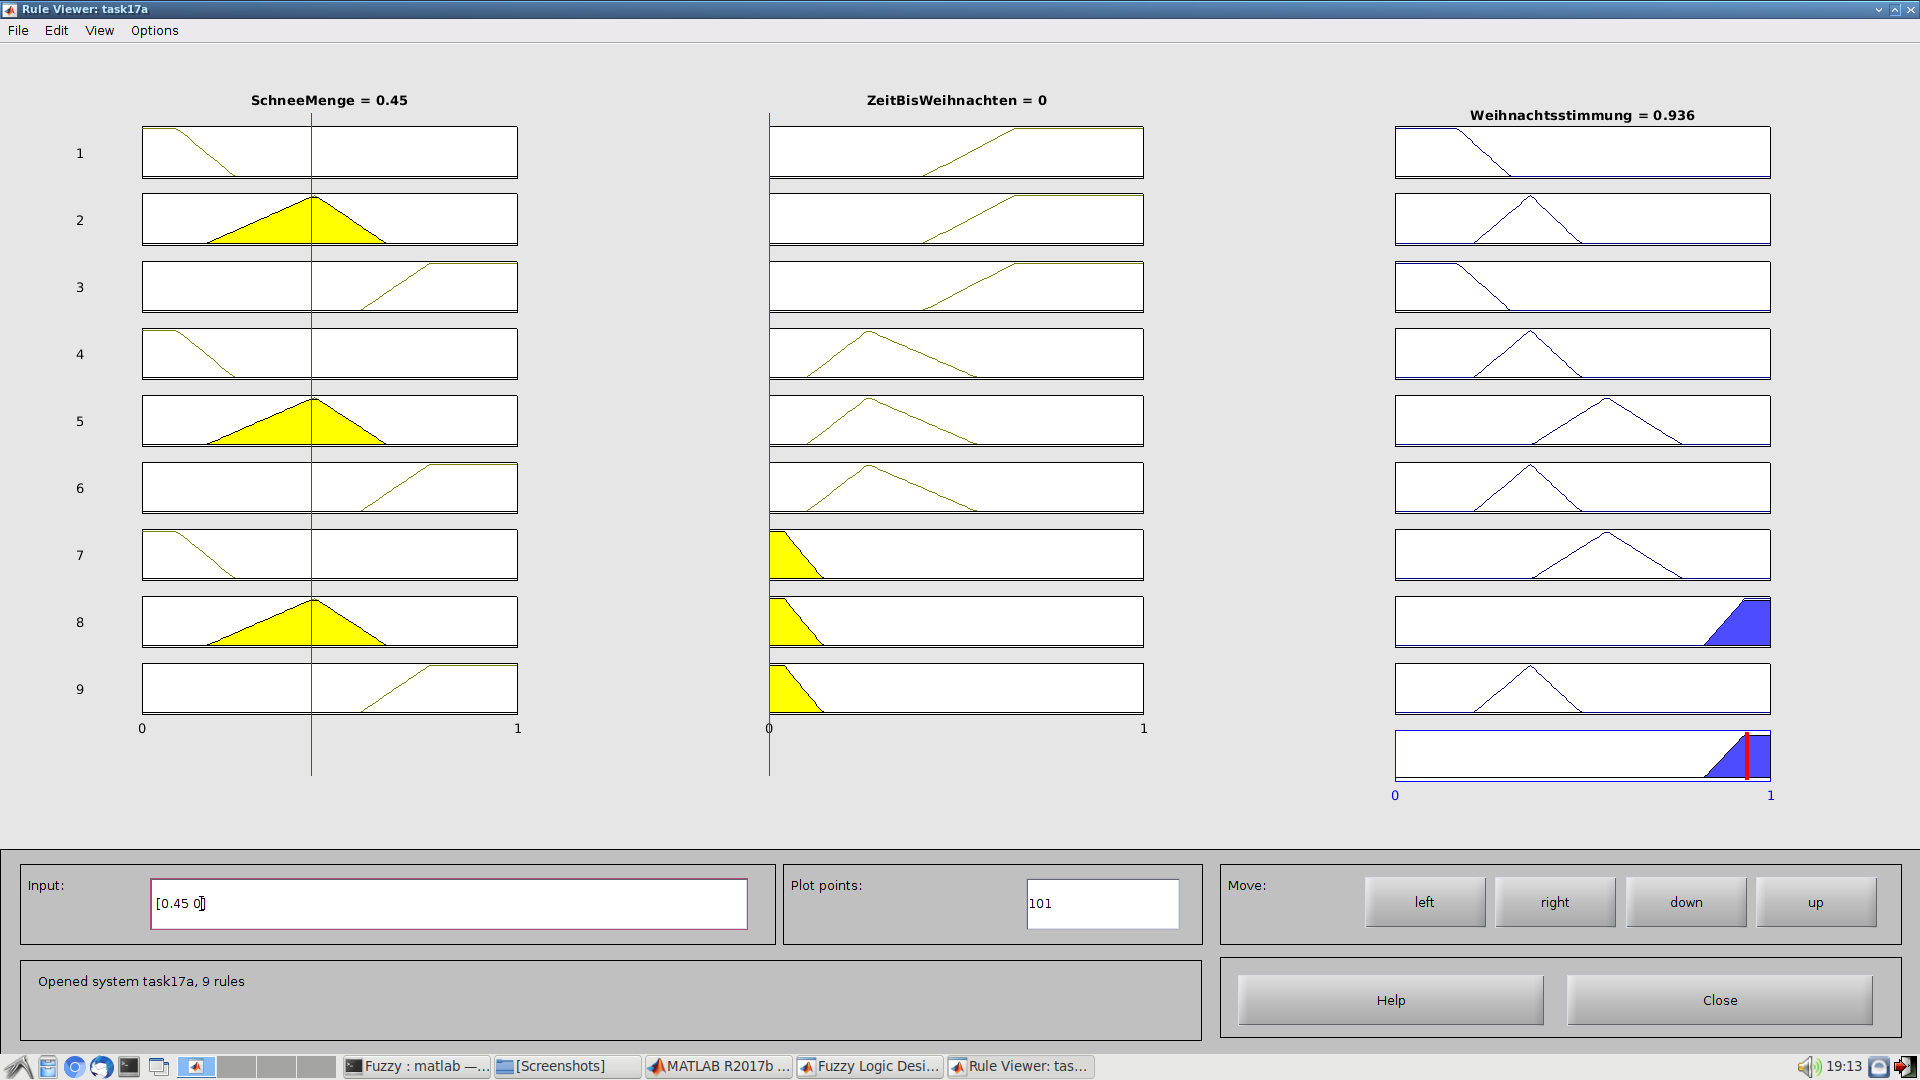
\includegraphics[width=\textwidth]{part/screenshots/fuzzy-17b-0,45-0}
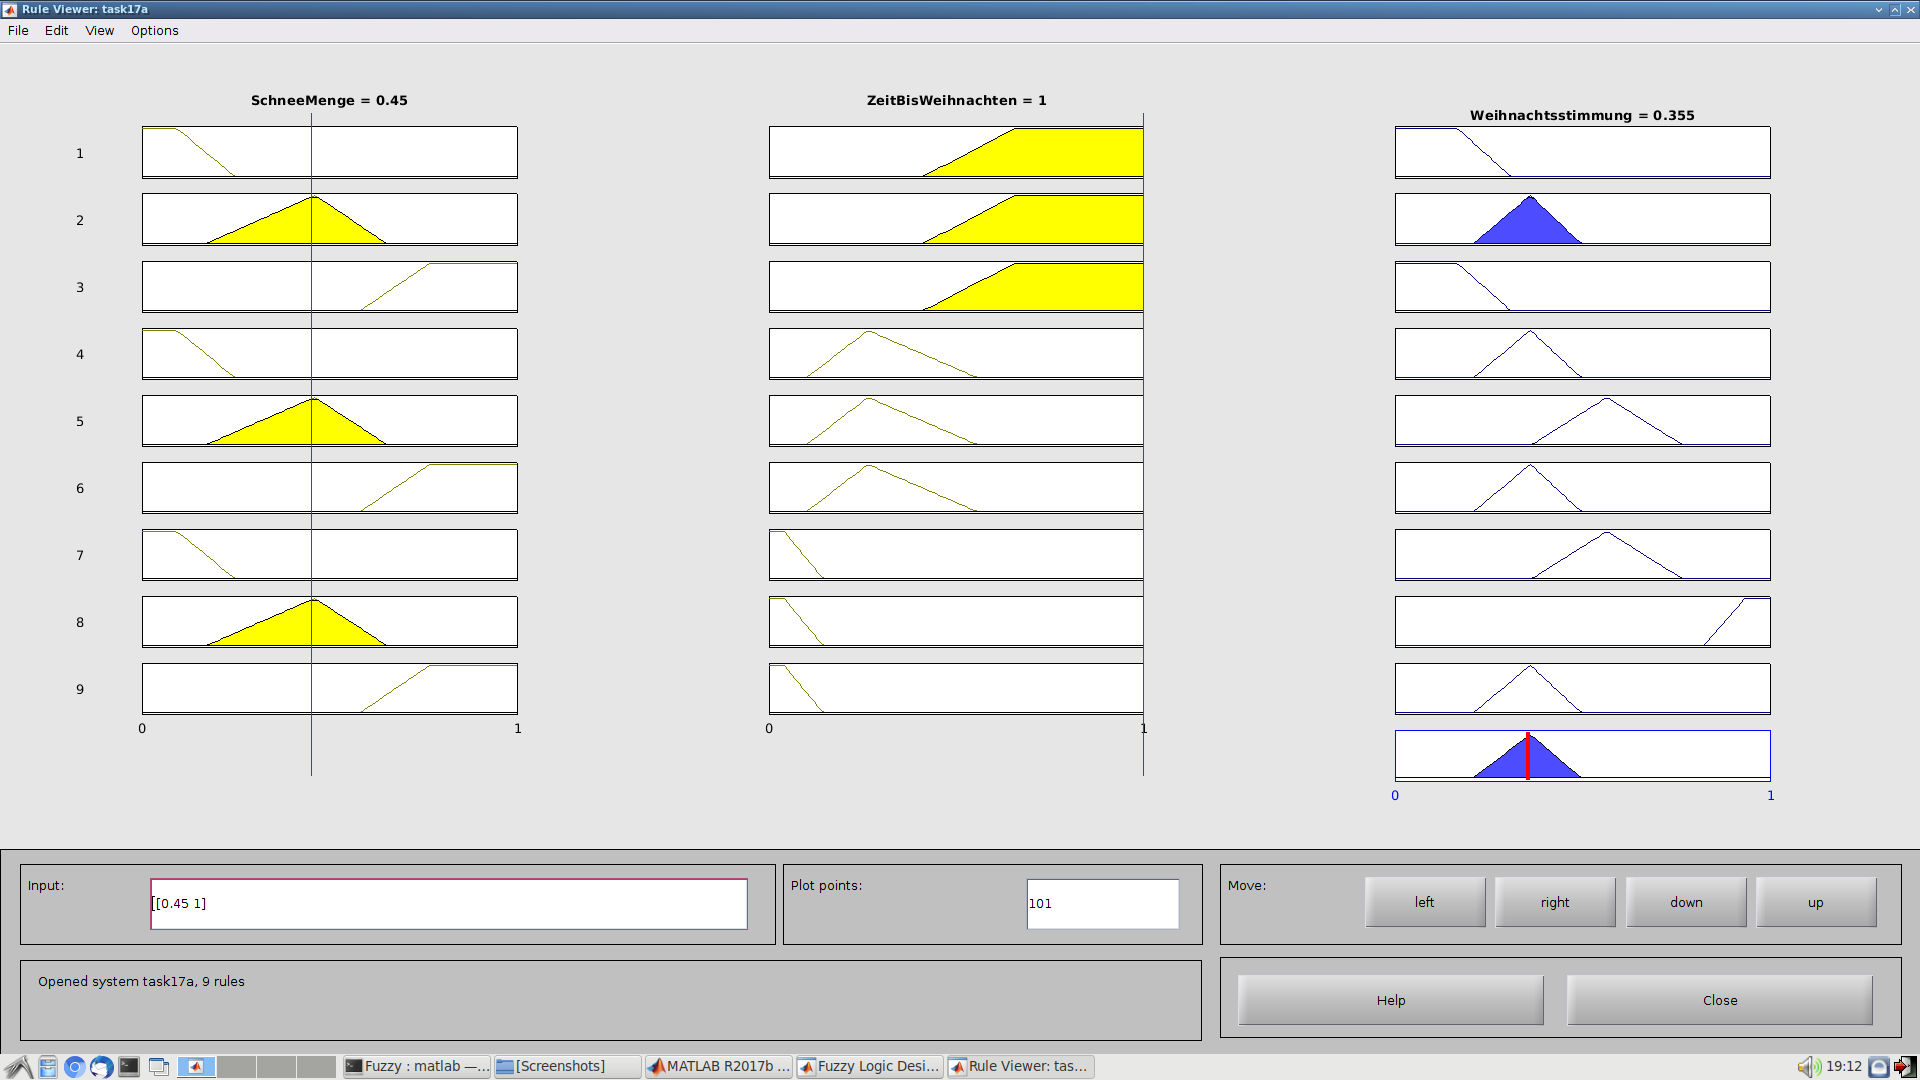
\includegraphics[width=\textwidth]{part/screenshots/fuzzy-17b-0,45-1}
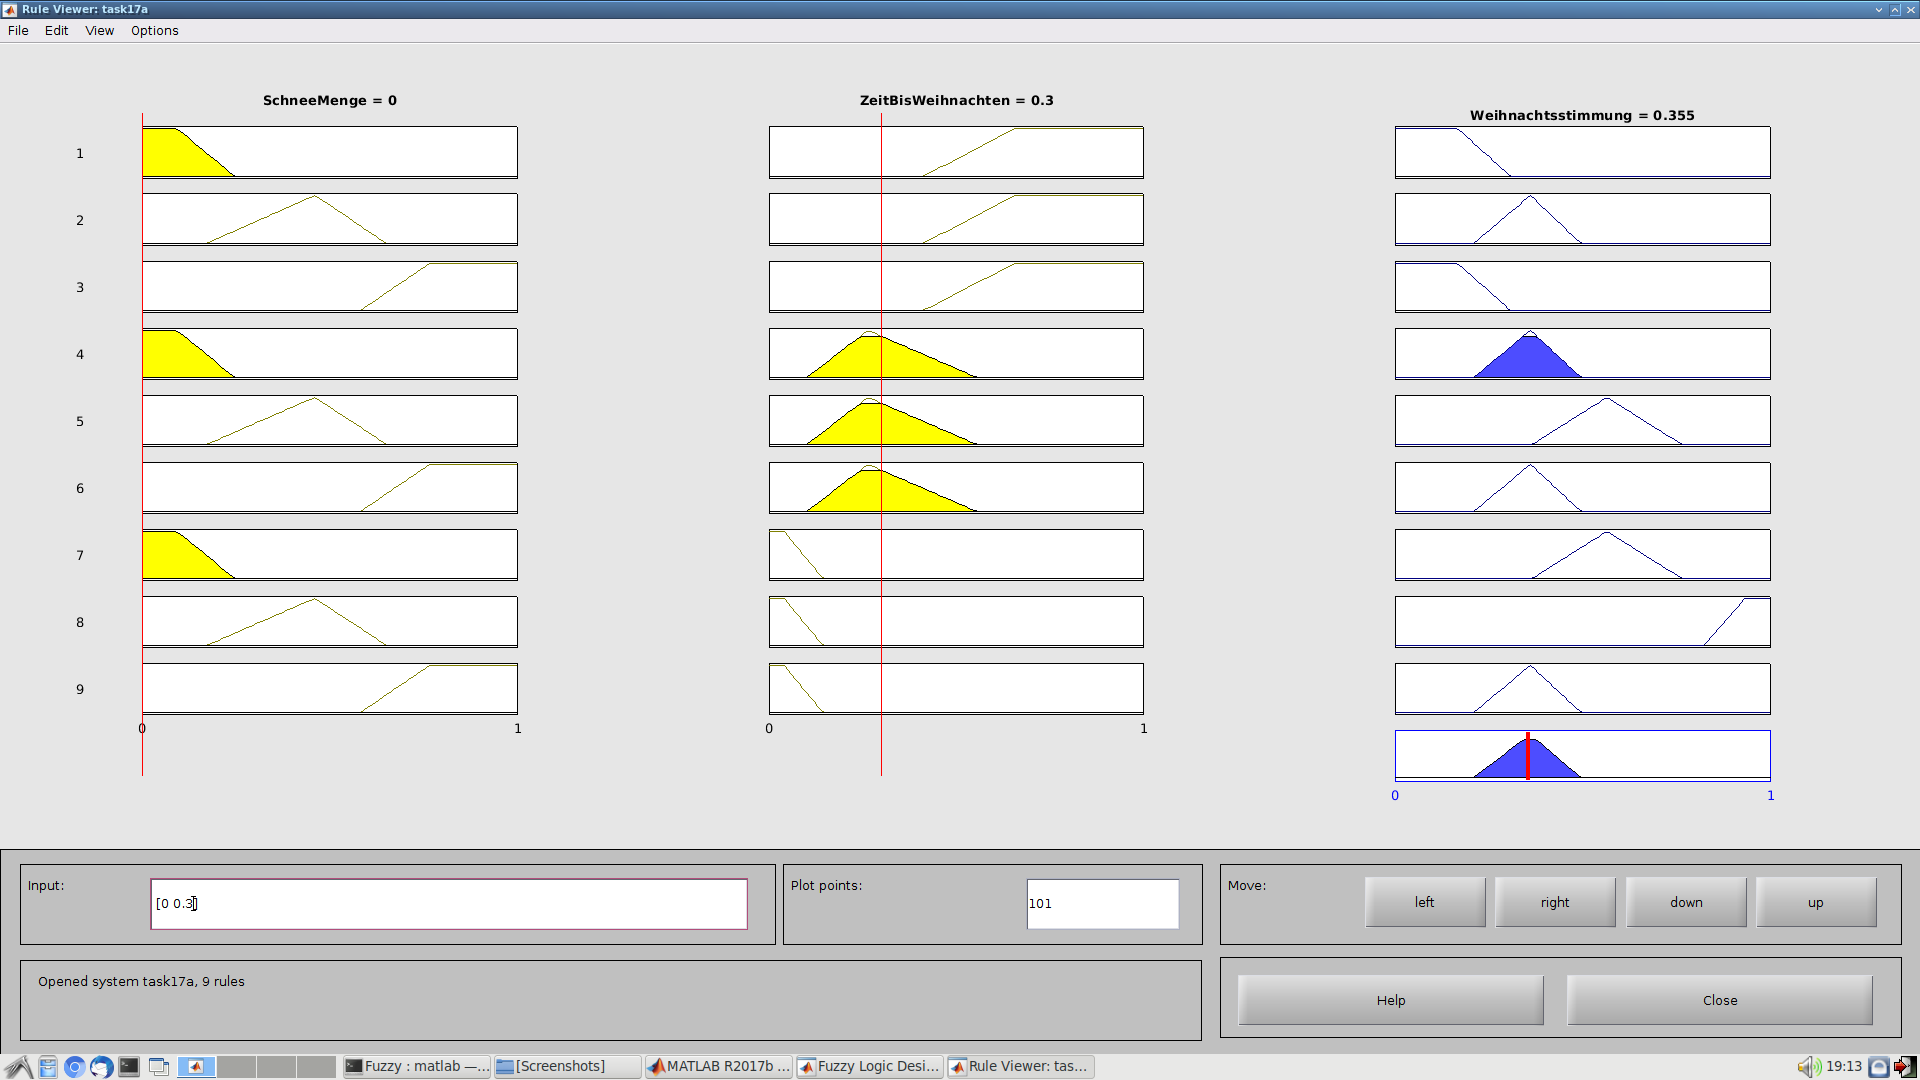
\includegraphics[width=\textwidth]{part/screenshots/fuzzy-17b-0-0,3}
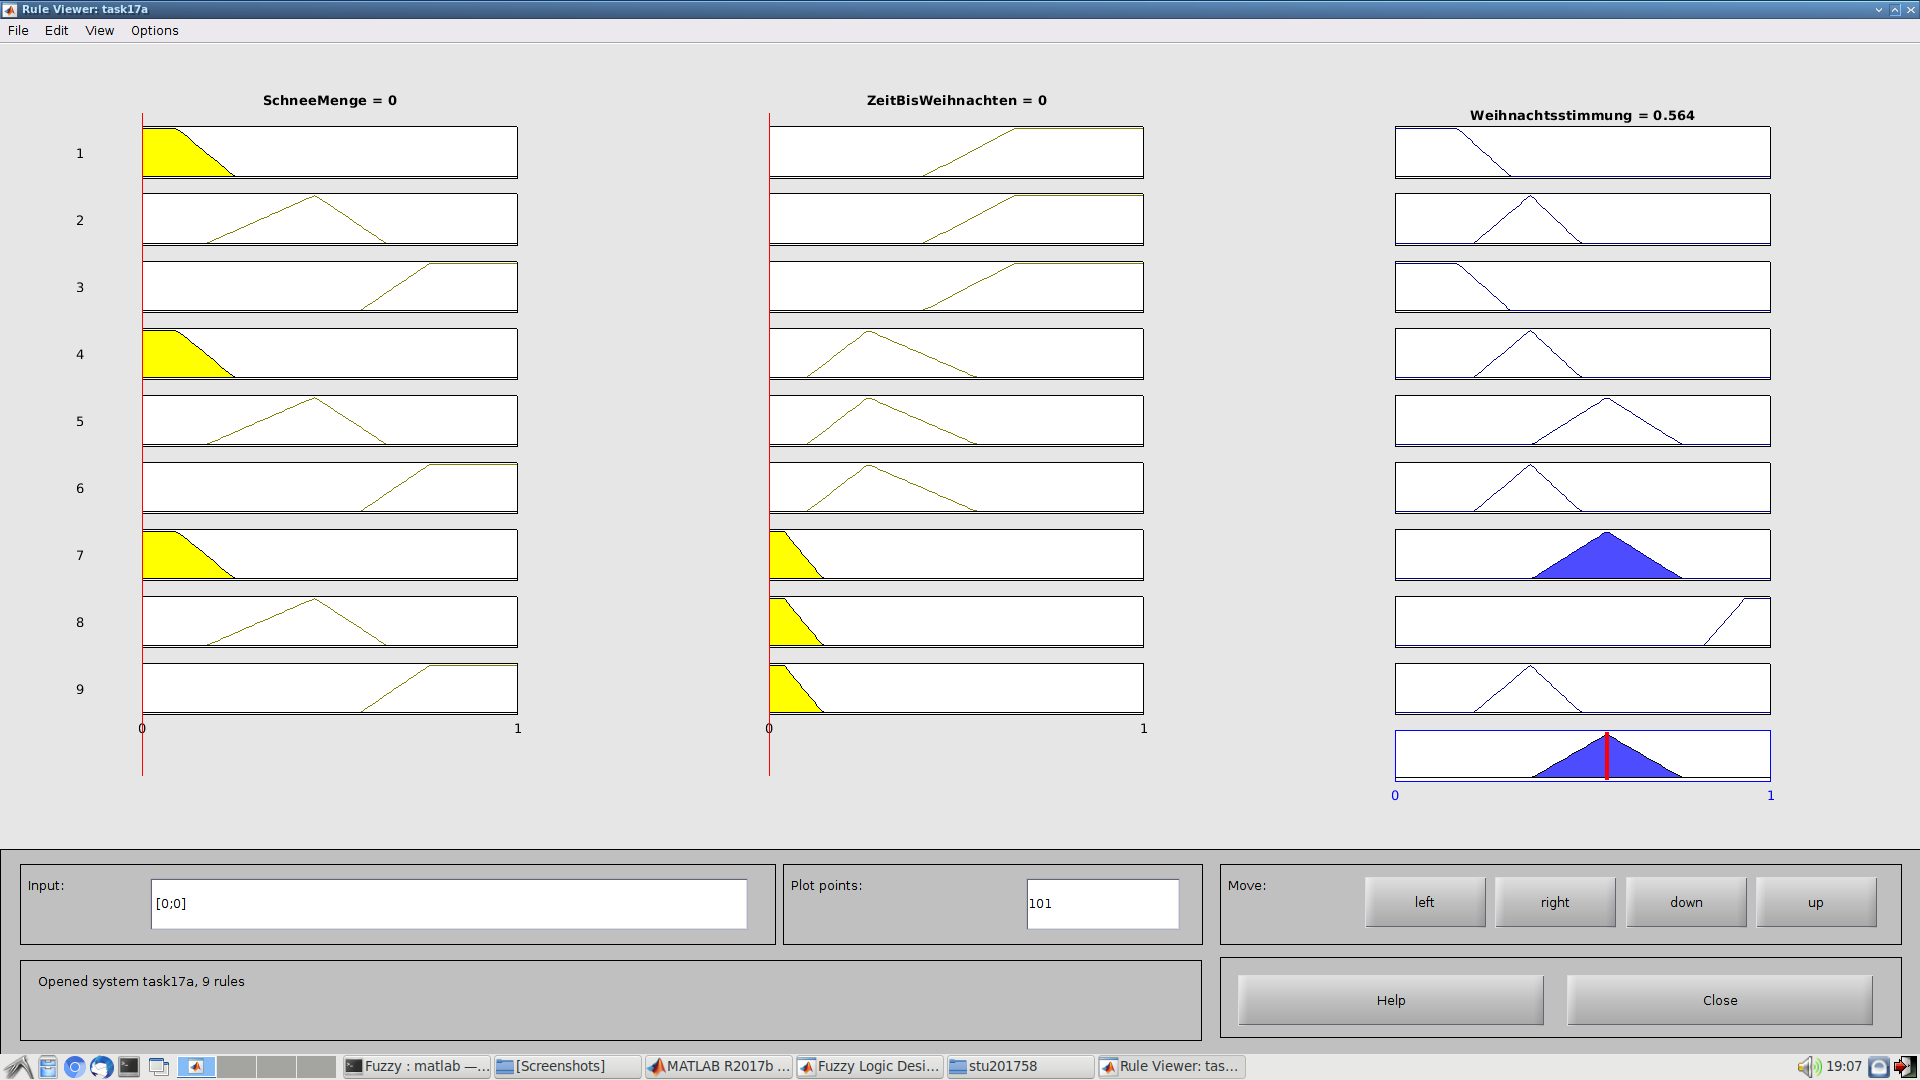
\includegraphics[width=\textwidth]{part/screenshots/fuzzy-17b-0-0}
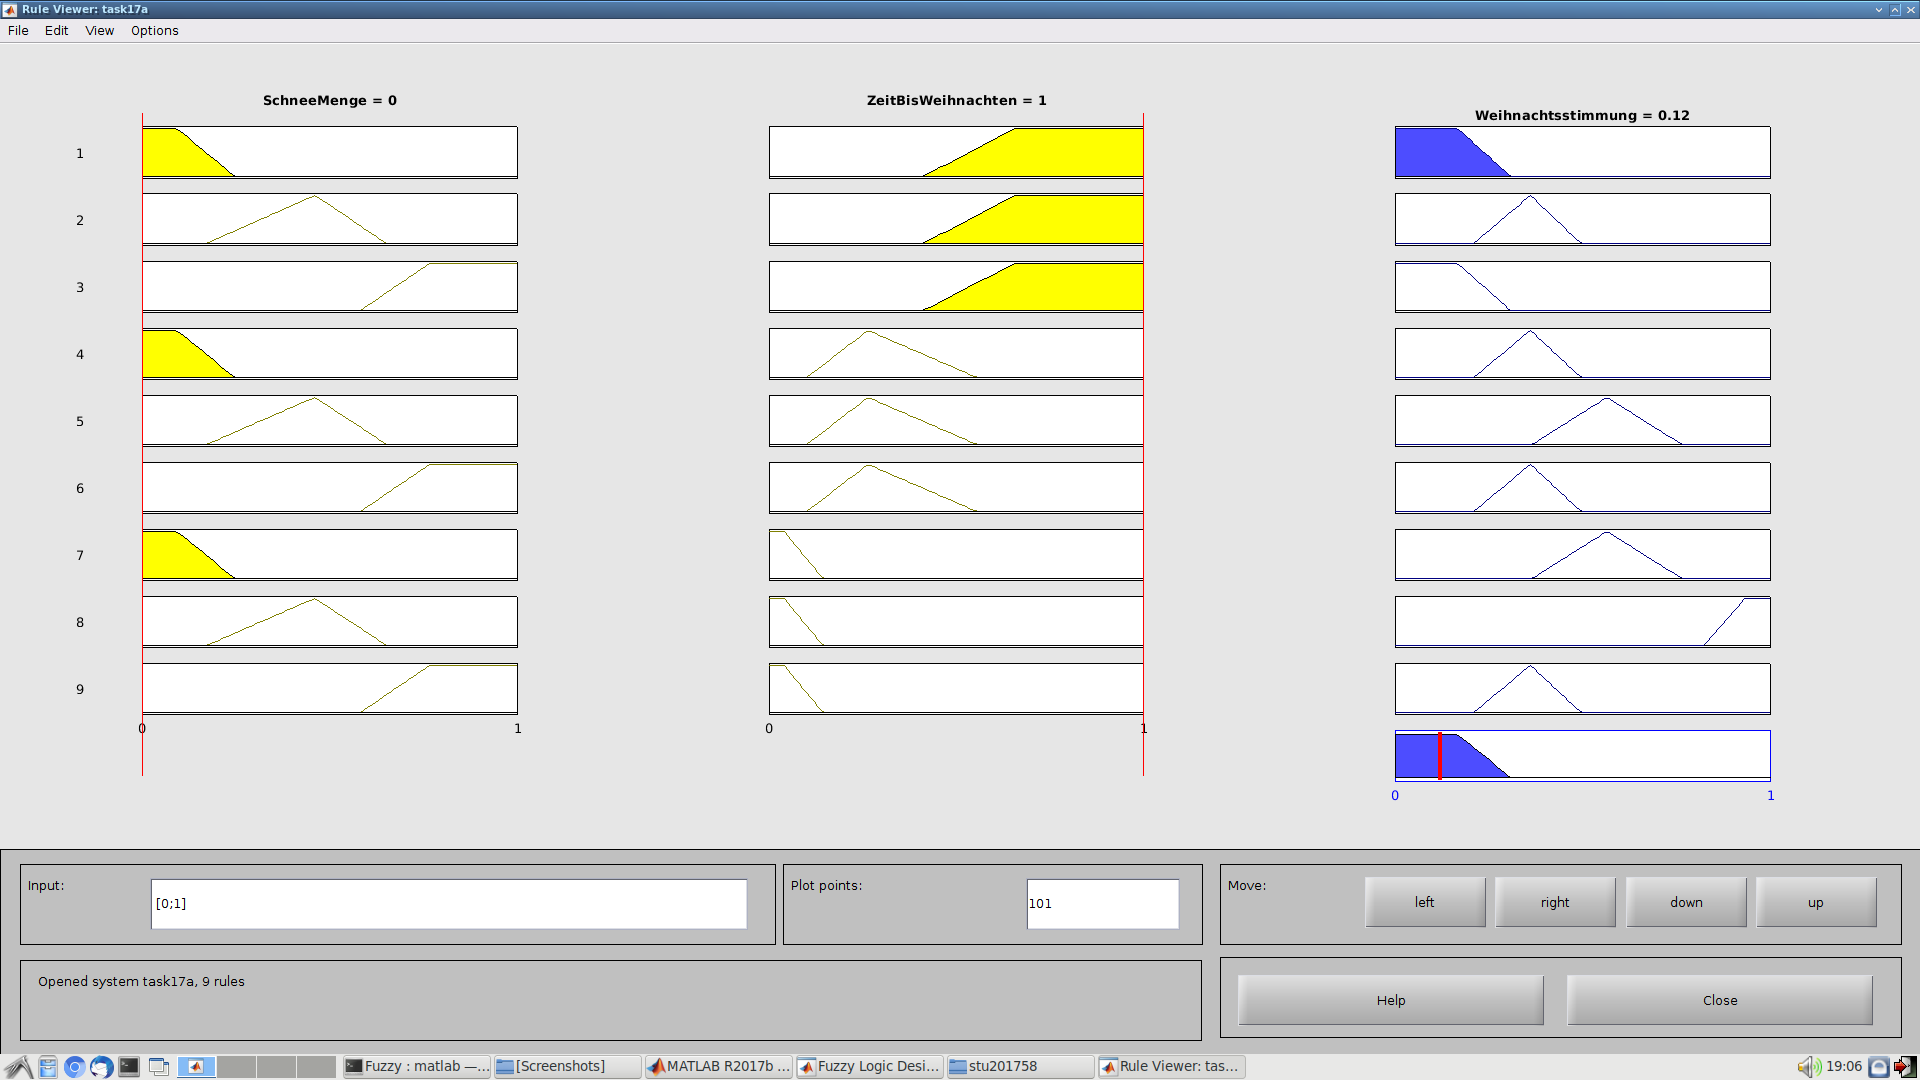
\includegraphics[width=\textwidth]{part/screenshots/fuzzy-17b-0-1}
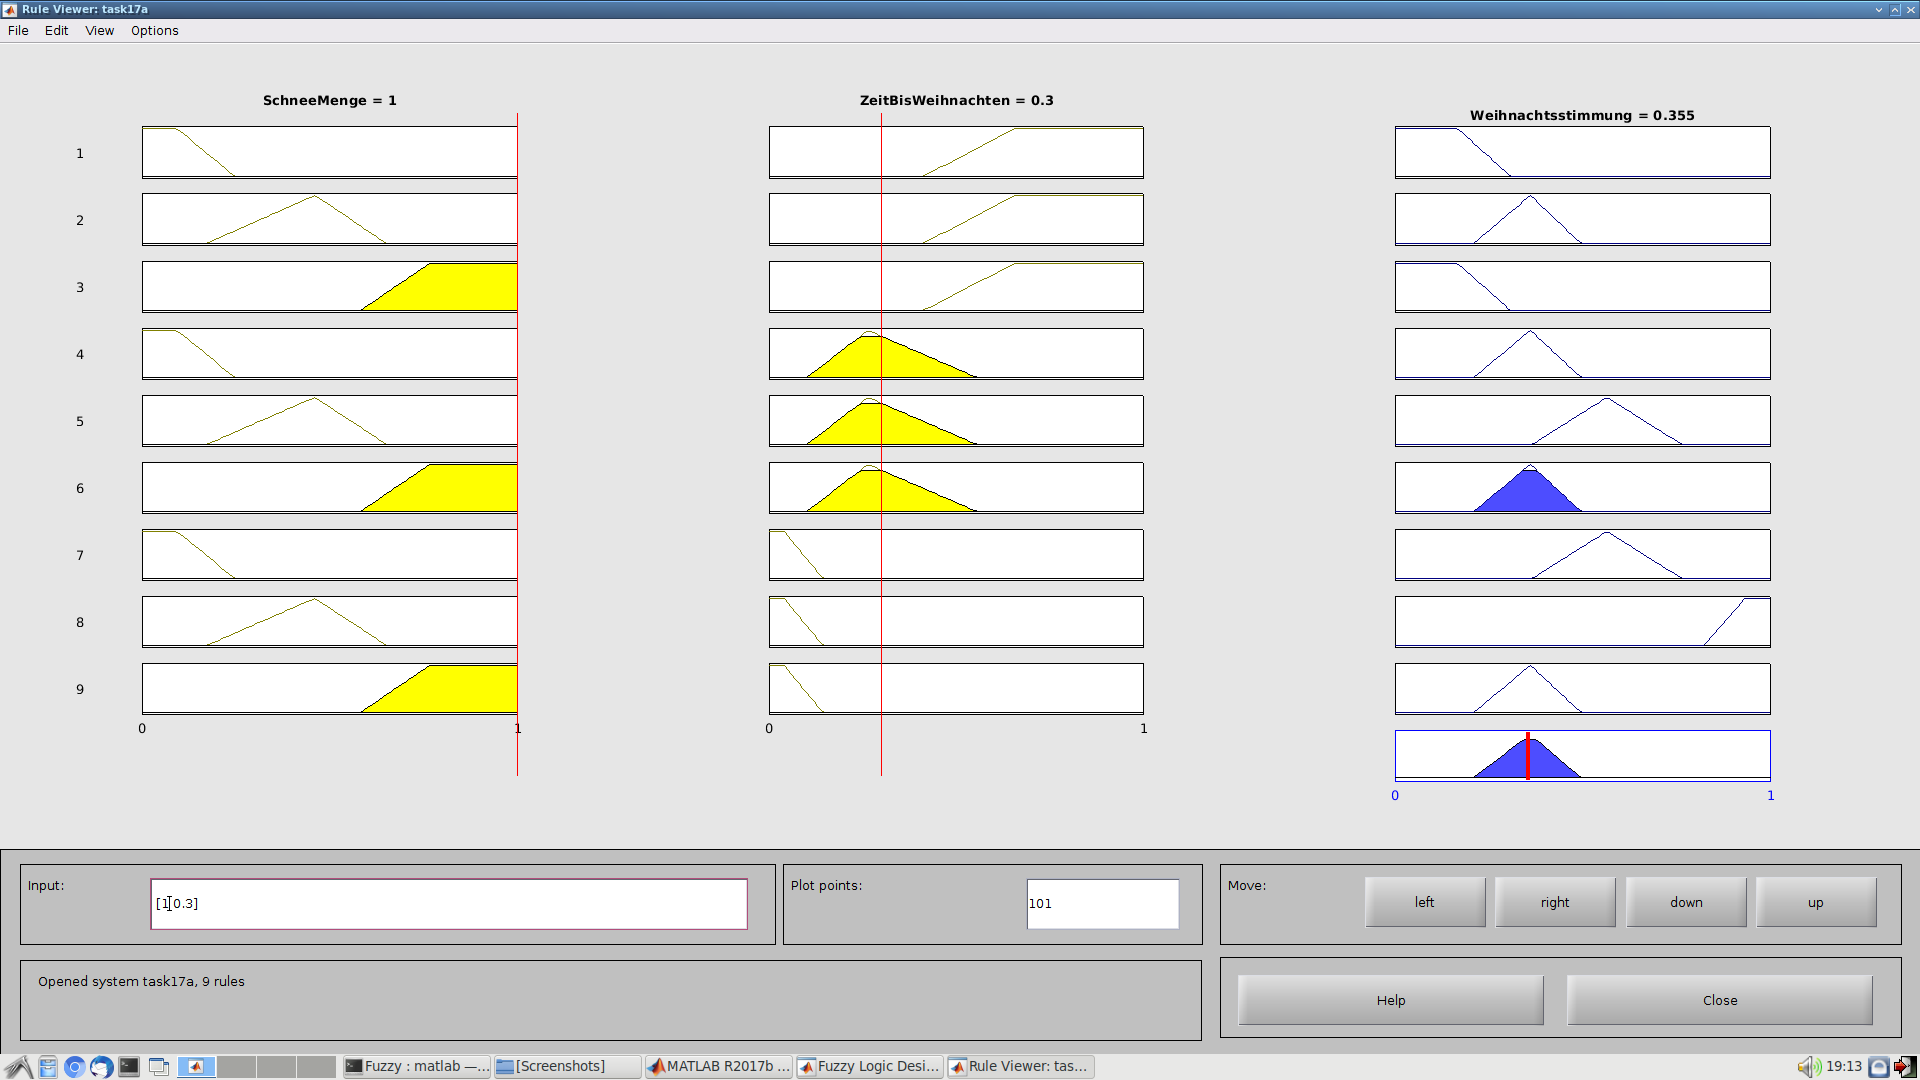
\includegraphics[width=\textwidth]{part/screenshots/fuzzy-17b-1-0,3}
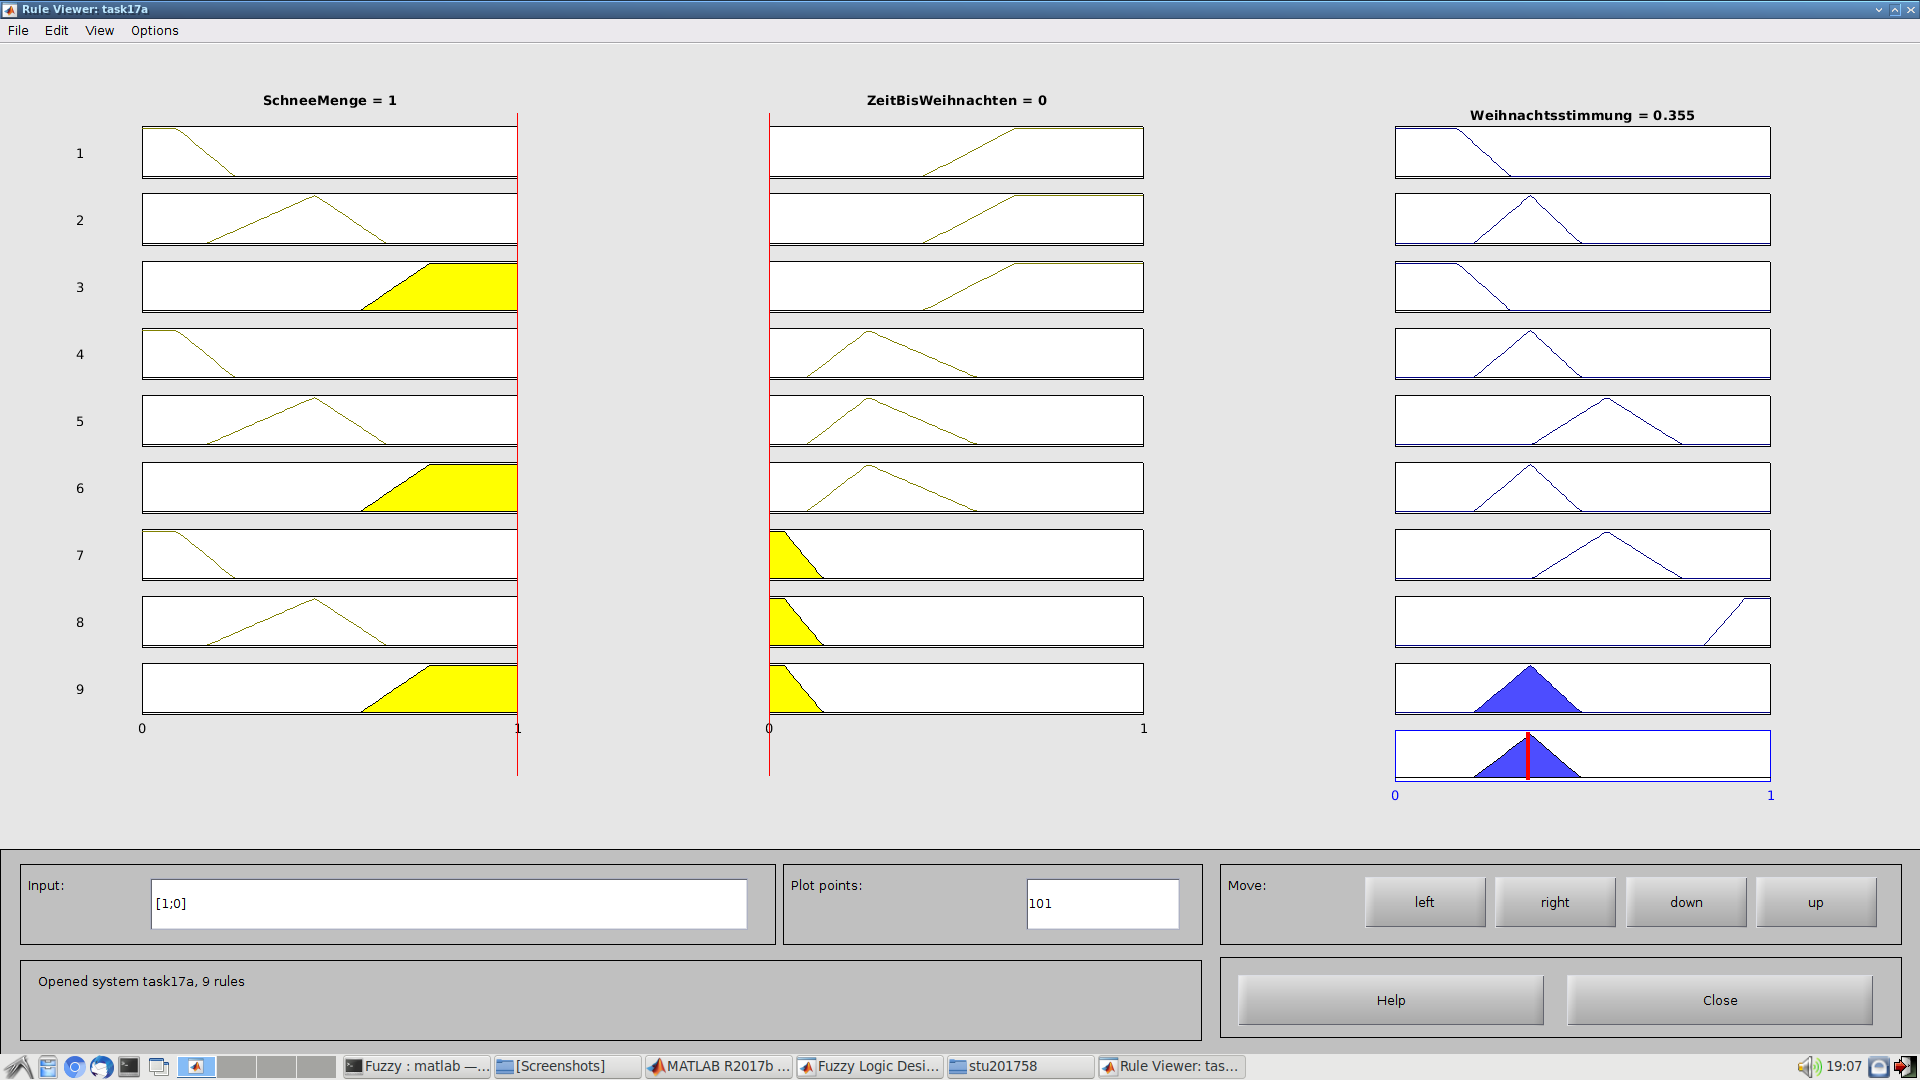
\includegraphics[width=\textwidth]{part/screenshots/fuzzy-17b-1-0}
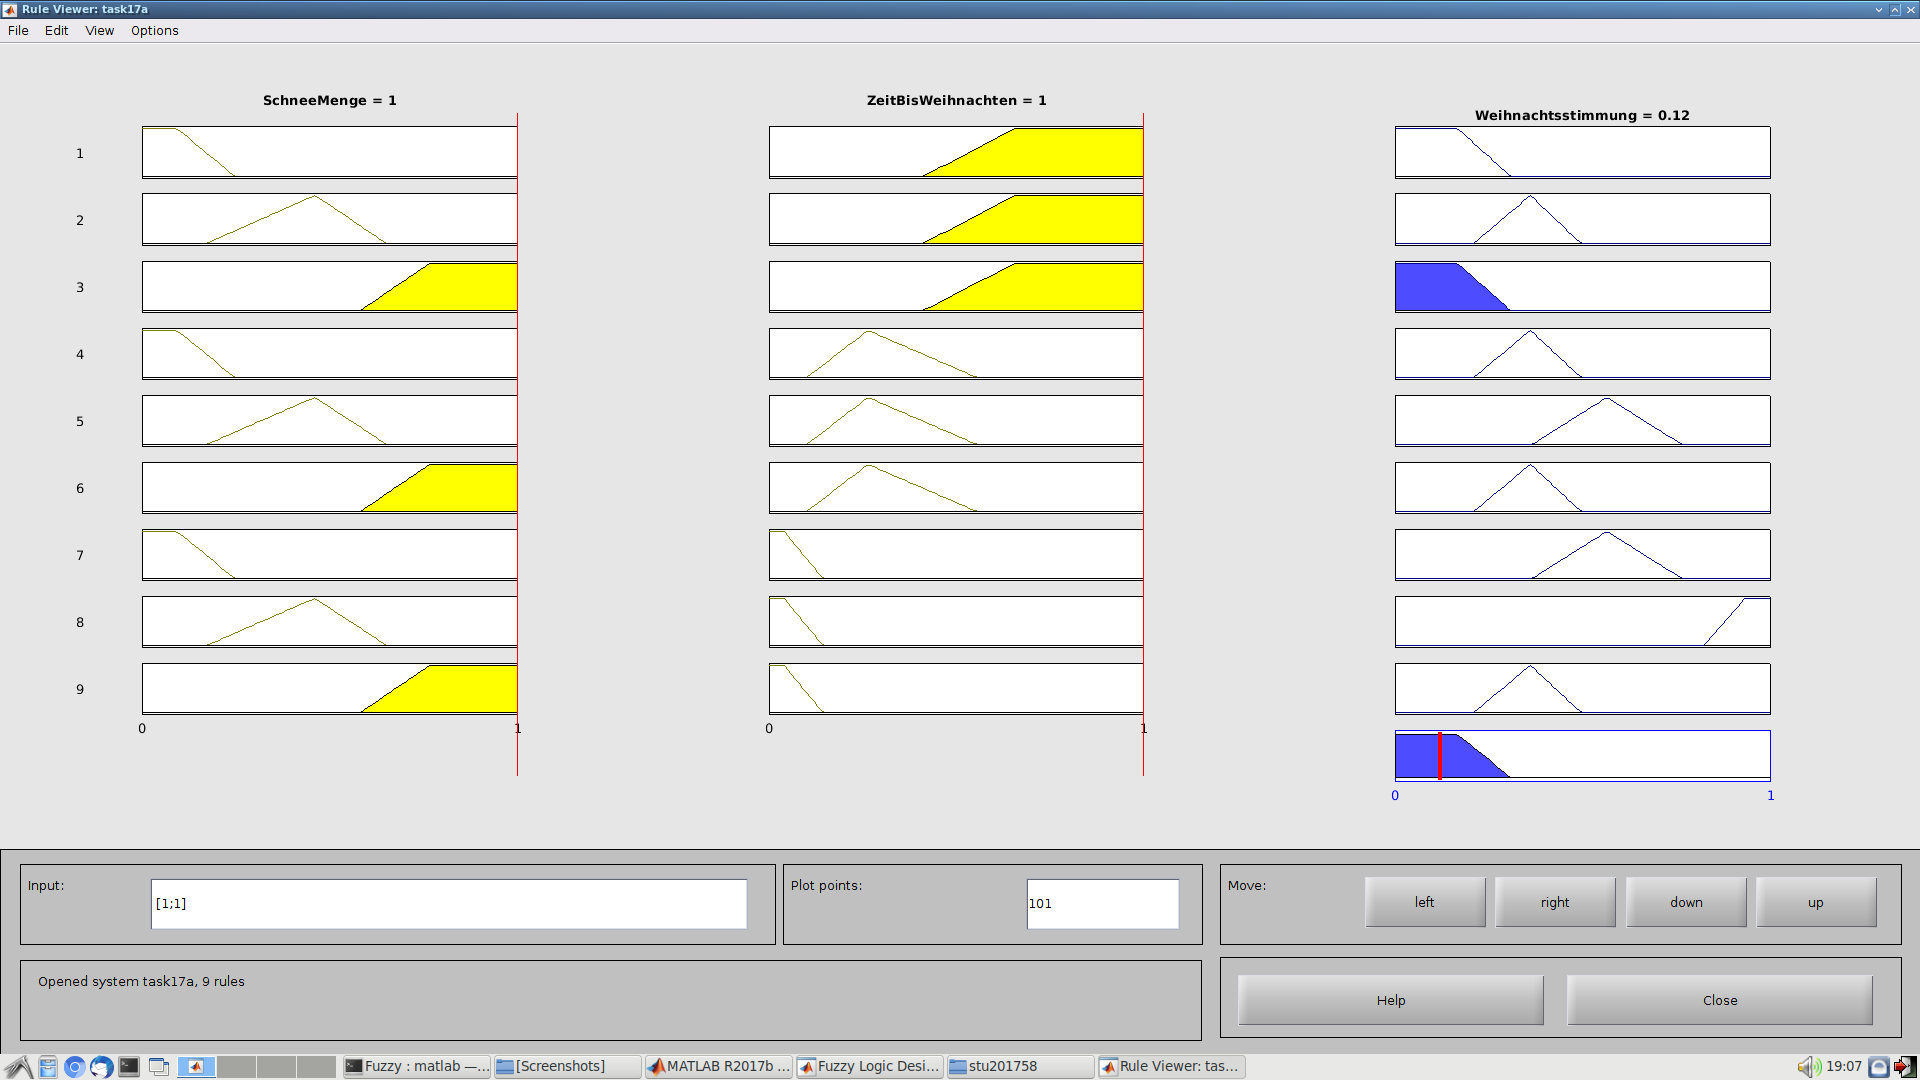
\includegraphics[width=\textwidth]{part/screenshots/fuzzy-17b-1-1}

\subsection*{c)}

\subsection*{K04}
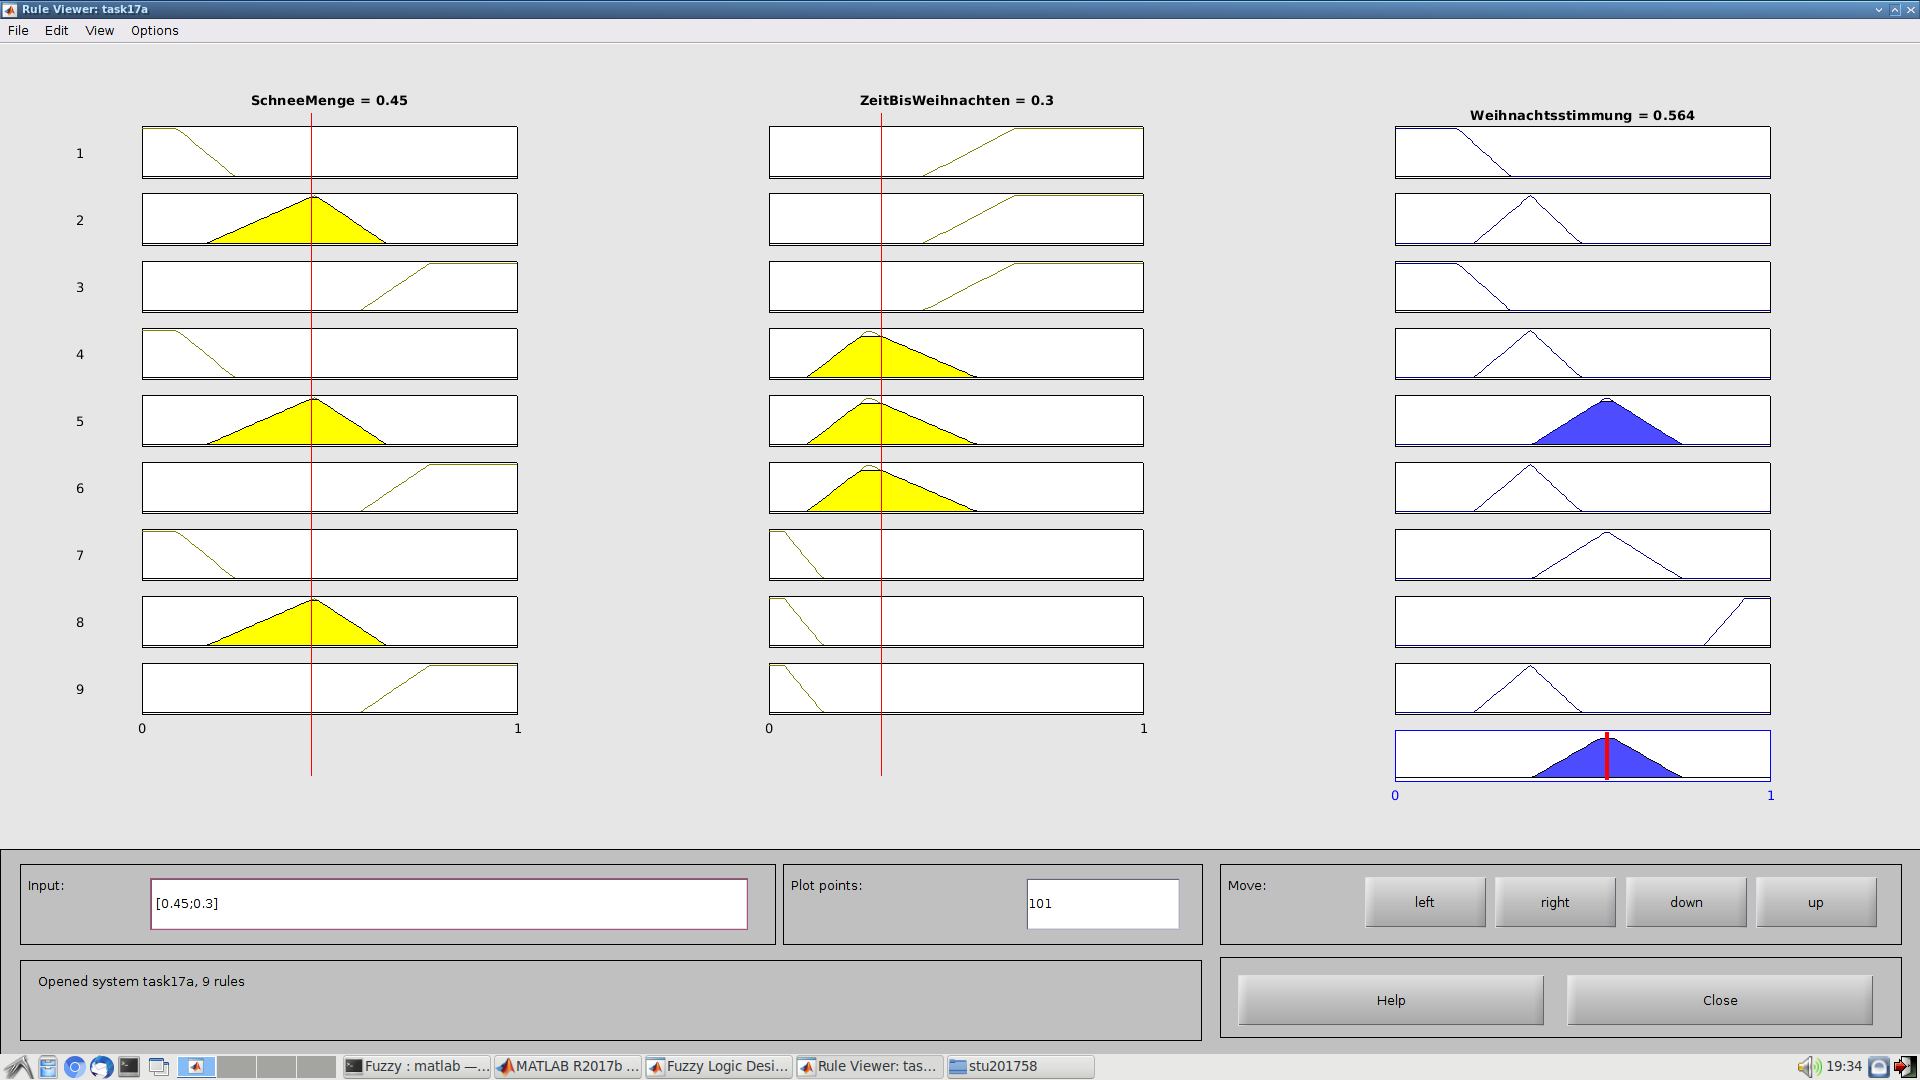
\includegraphics[width=\textwidth]{part/screenshots/fuzzy-17c-K04-0,45-0,3}
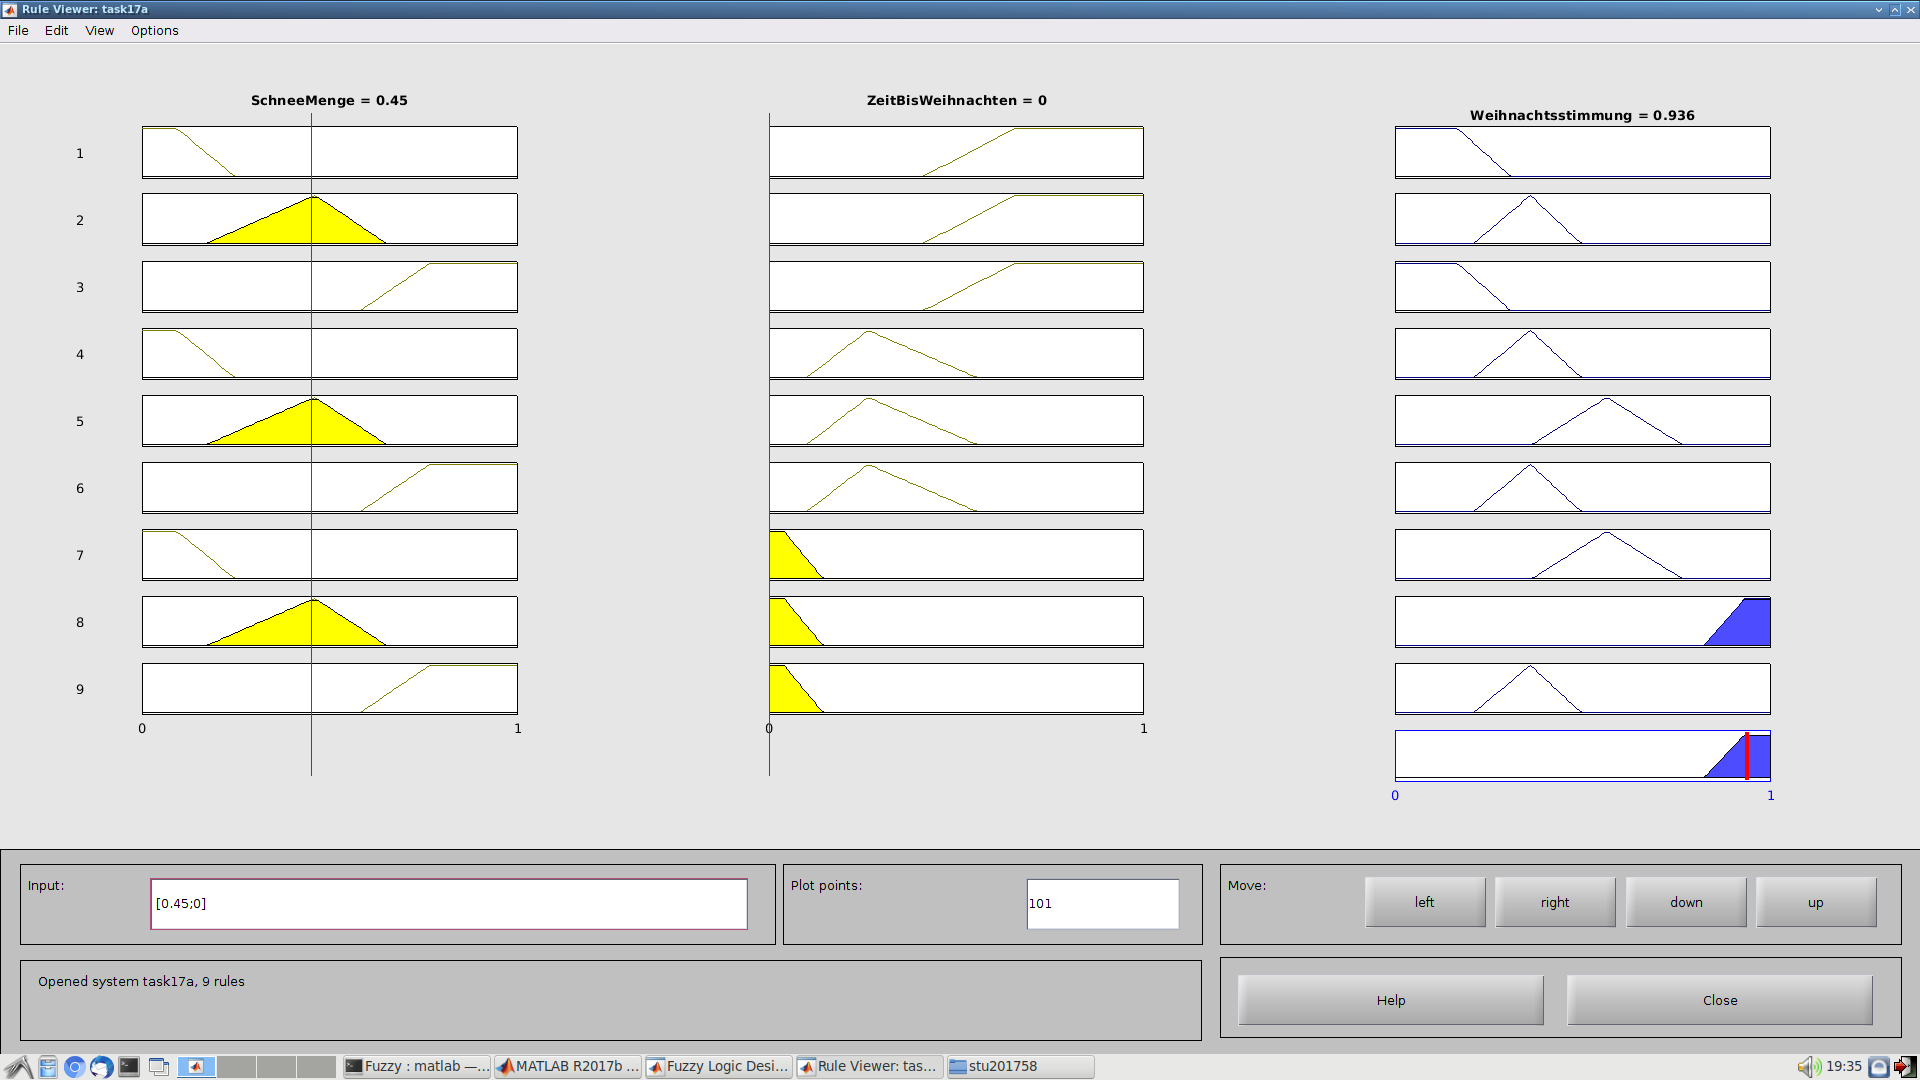
\includegraphics[width=\textwidth]{part/screenshots/fuzzy-17c-K04-0,45-0}
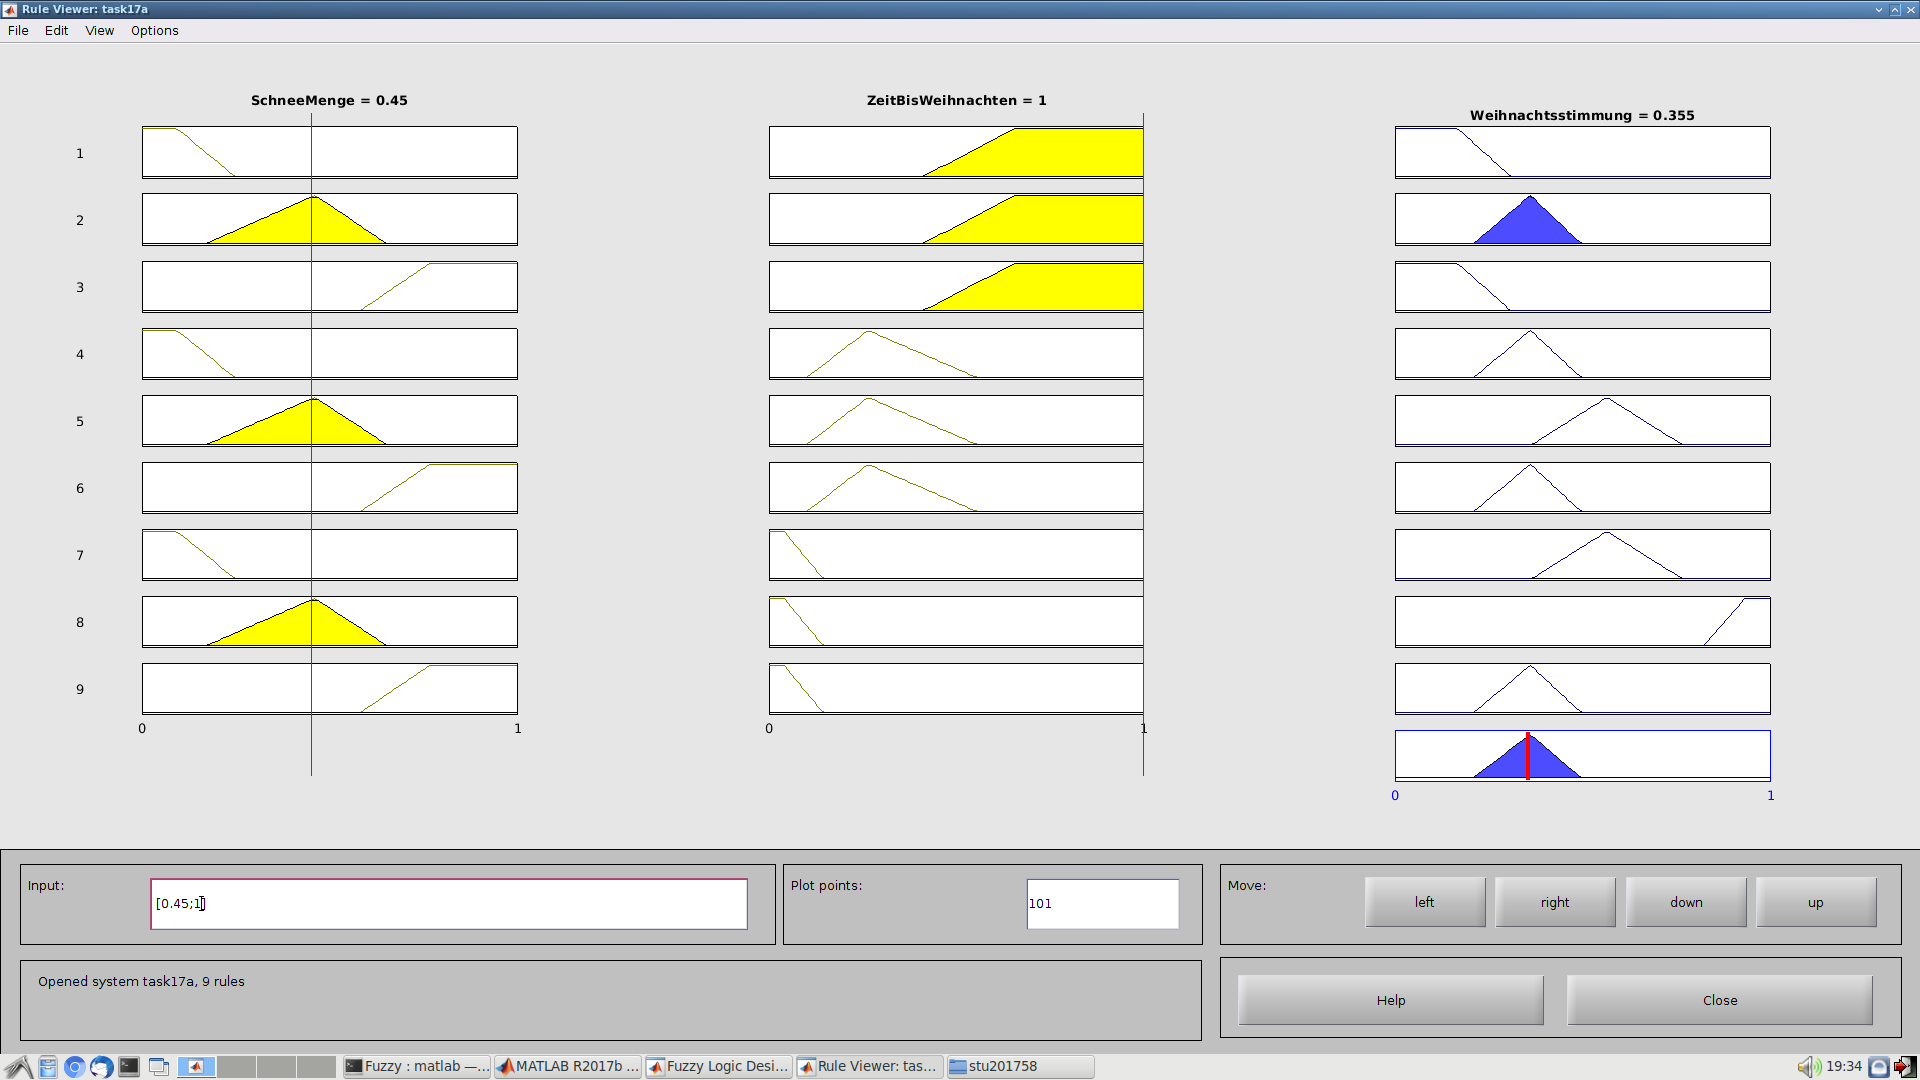
\includegraphics[width=\textwidth]{part/screenshots/fuzzy-17c-K04-0,45-1}
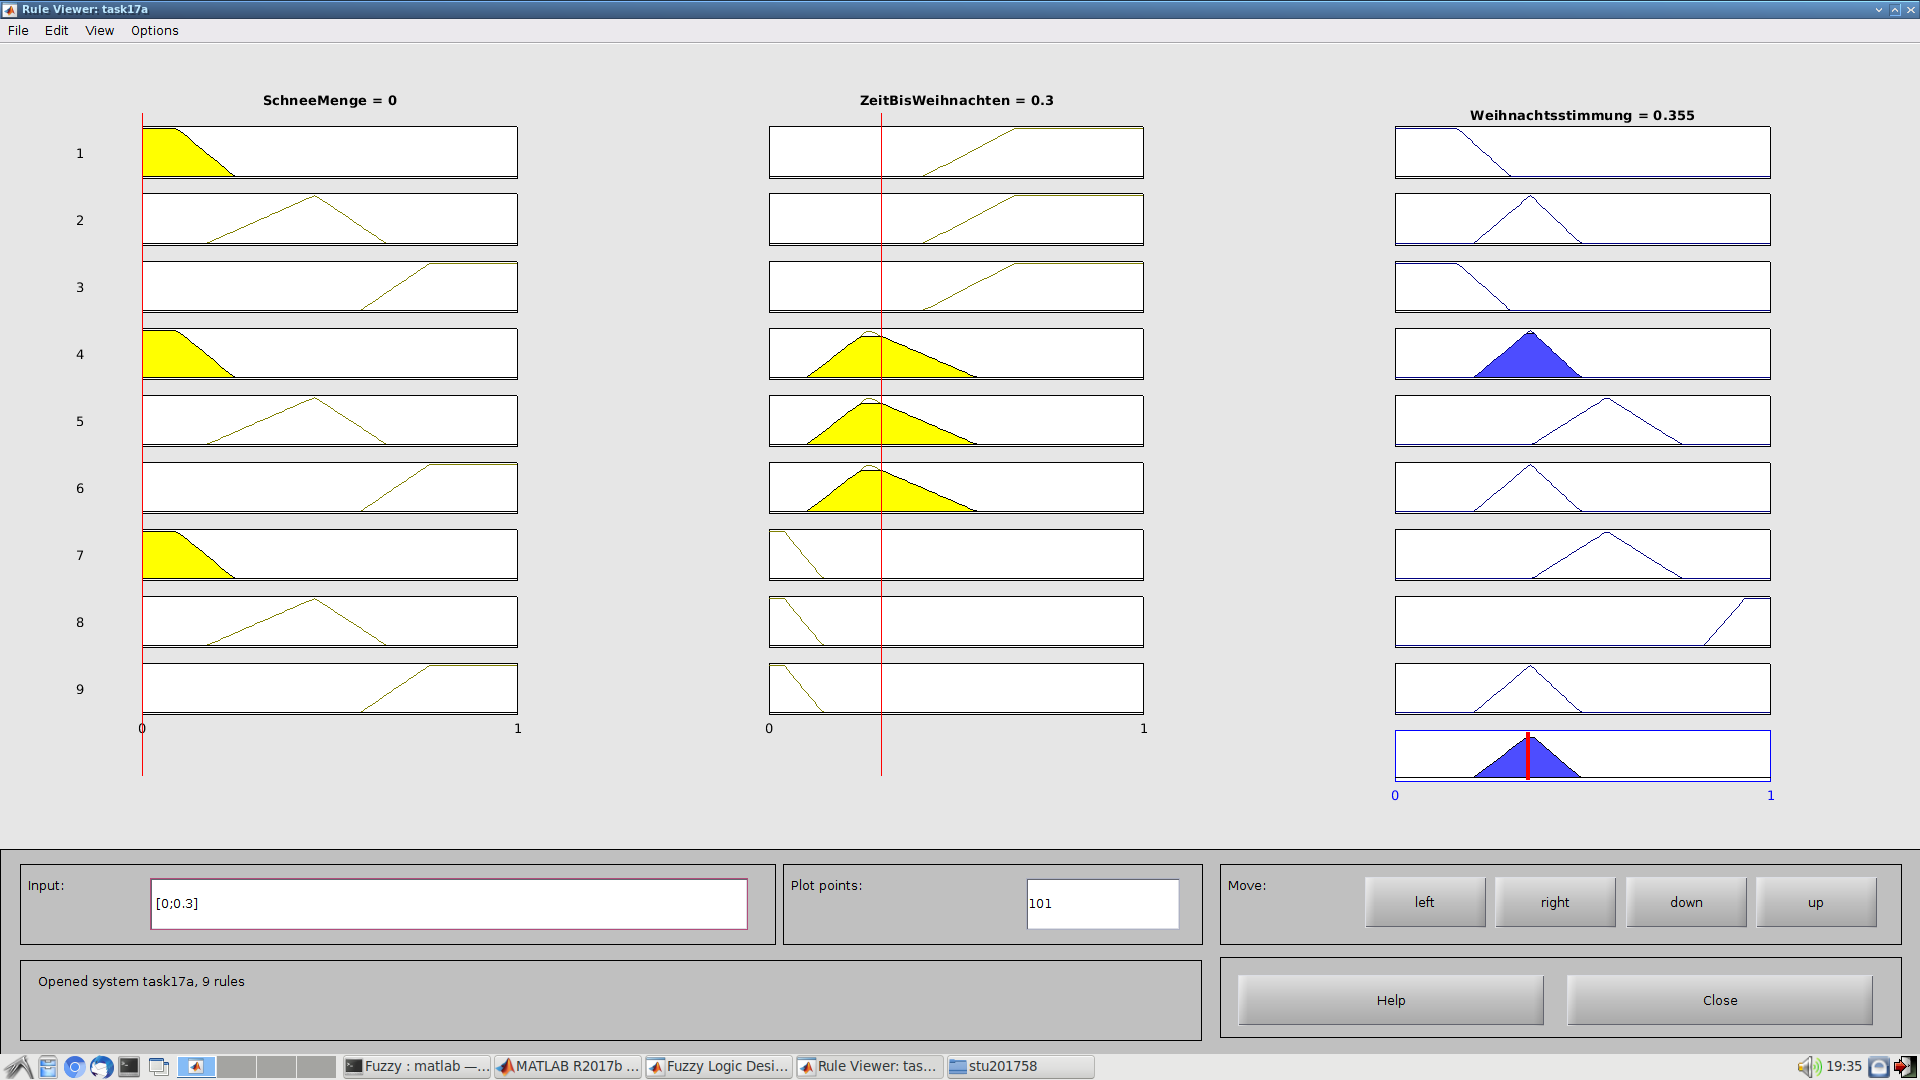
\includegraphics[width=\textwidth]{part/screenshots/fuzzy-17c-K04-0-0,3}
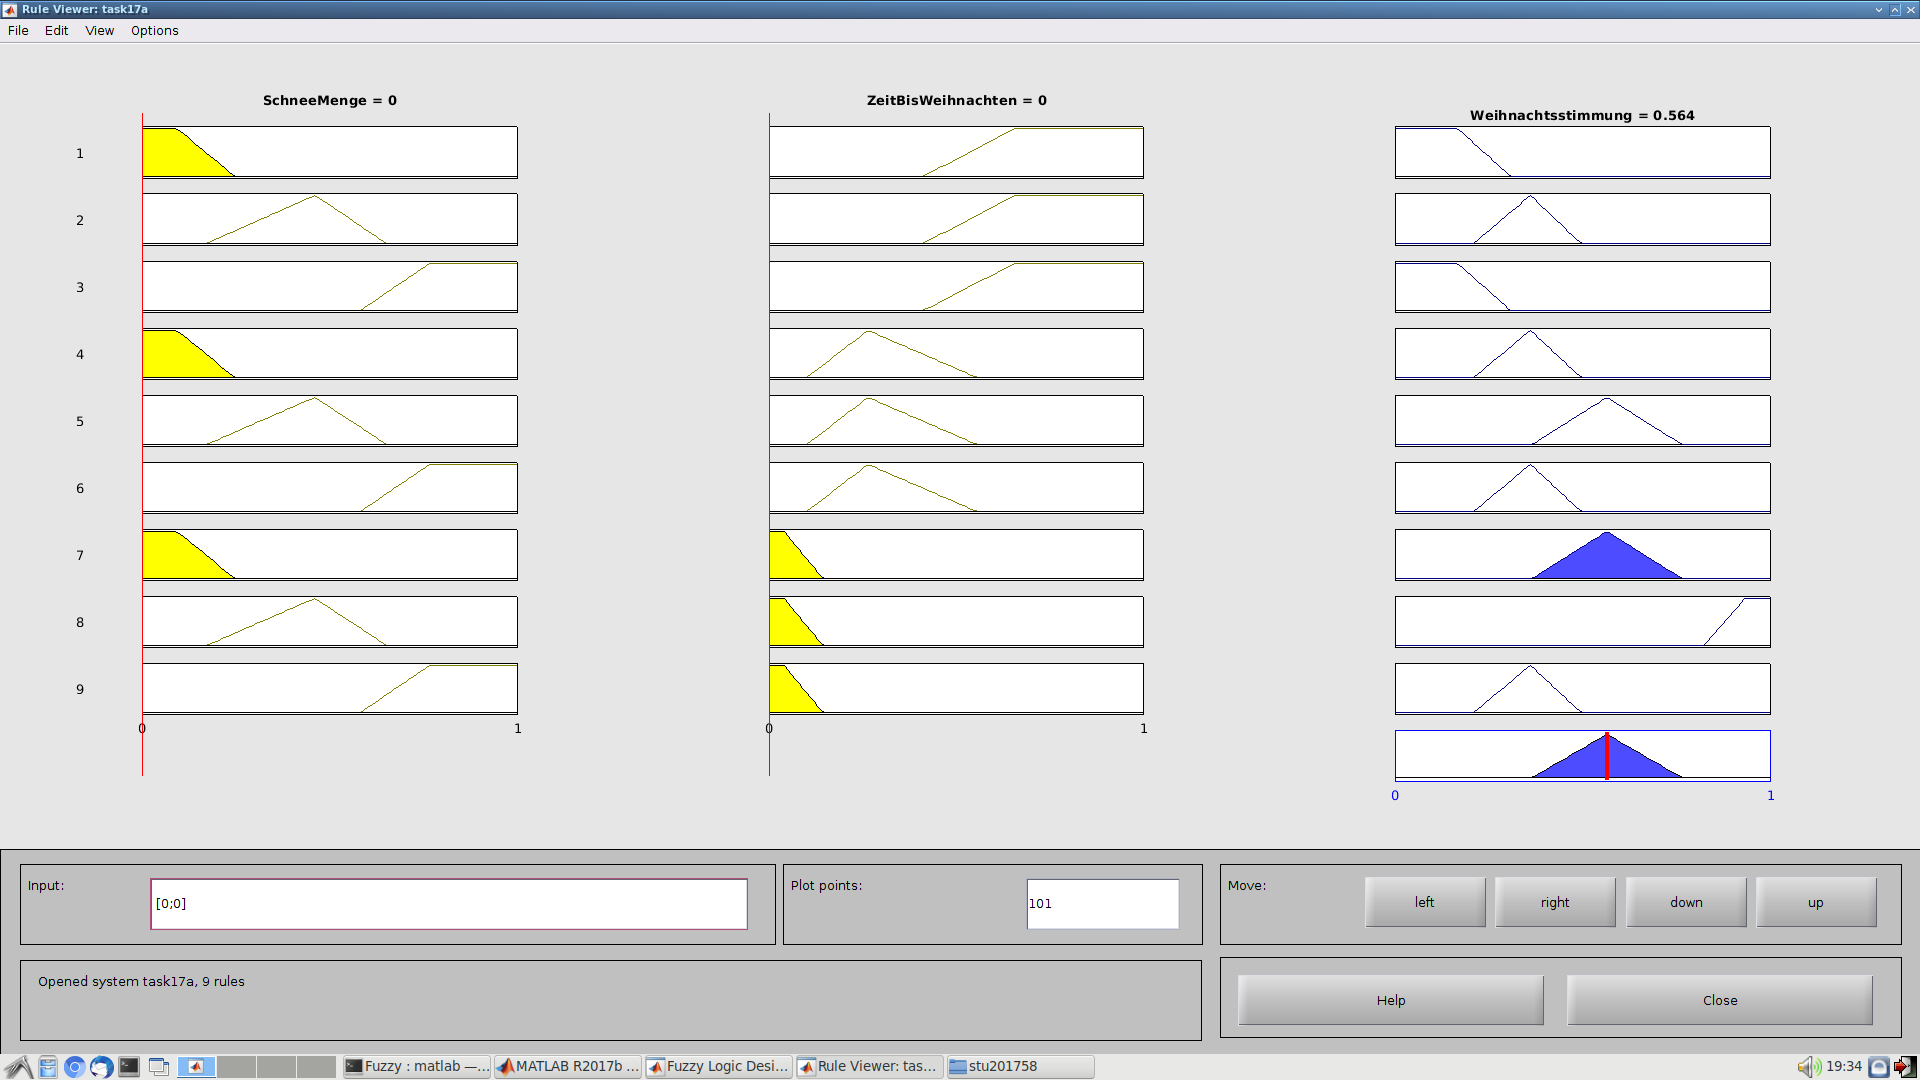
\includegraphics[width=\textwidth]{part/screenshots/fuzzy-17c-K04-0-0}
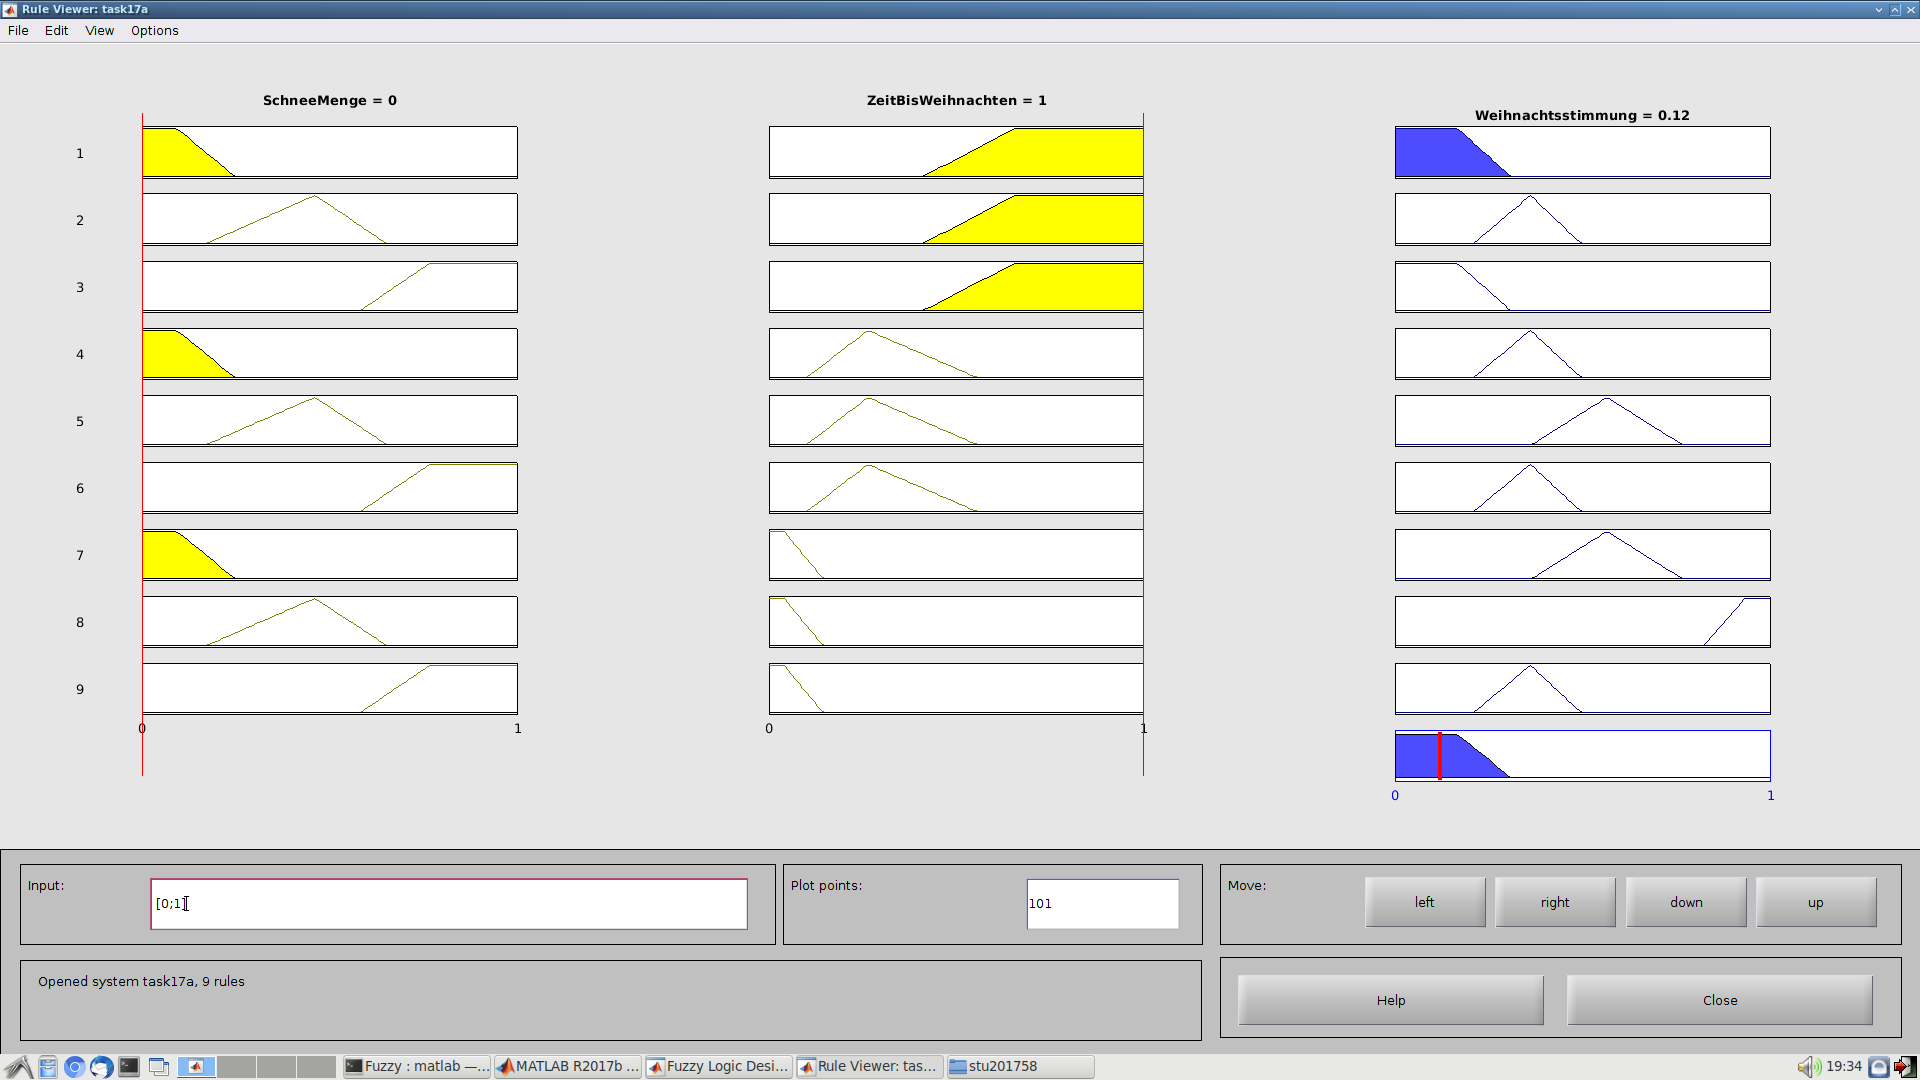
\includegraphics[width=\textwidth]{part/screenshots/fuzzy-17c-K04-0-1}
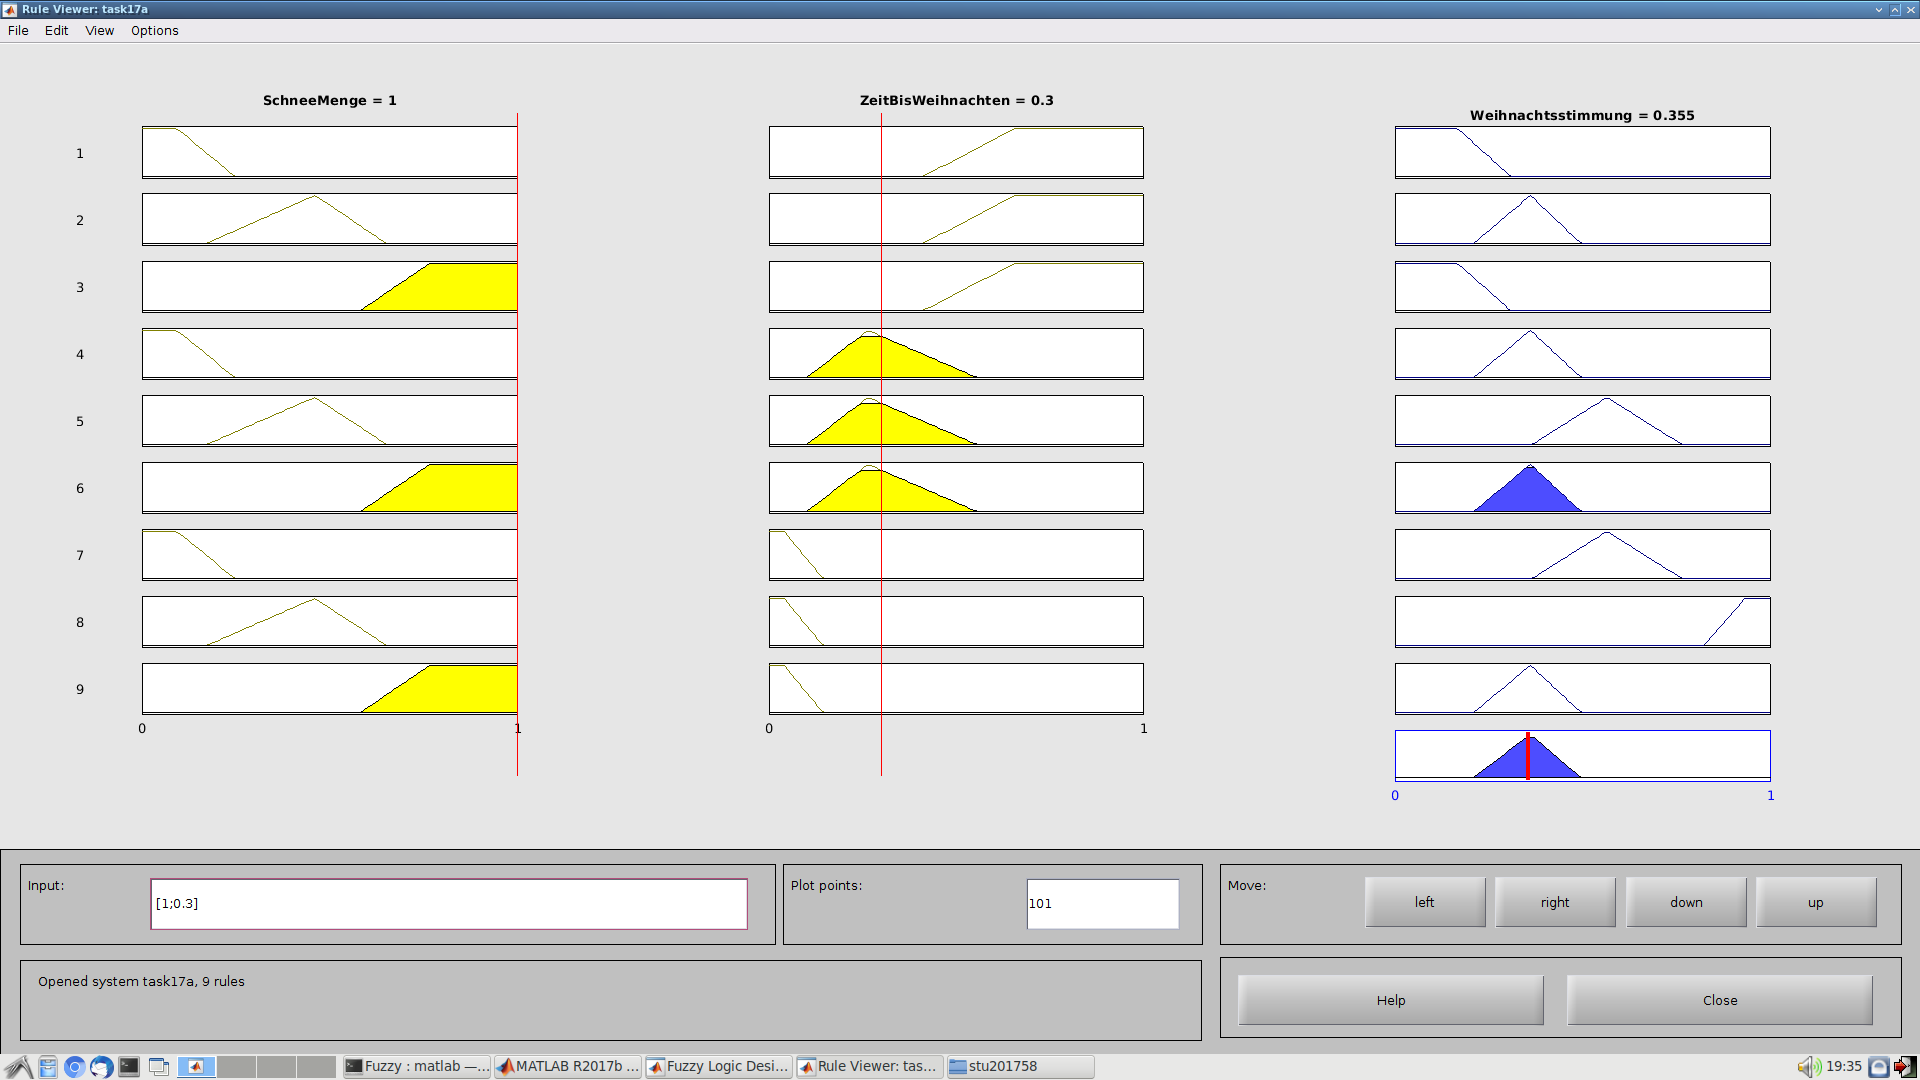
\includegraphics[width=\textwidth]{part/screenshots/fuzzy-17c-K04-1-0,3}
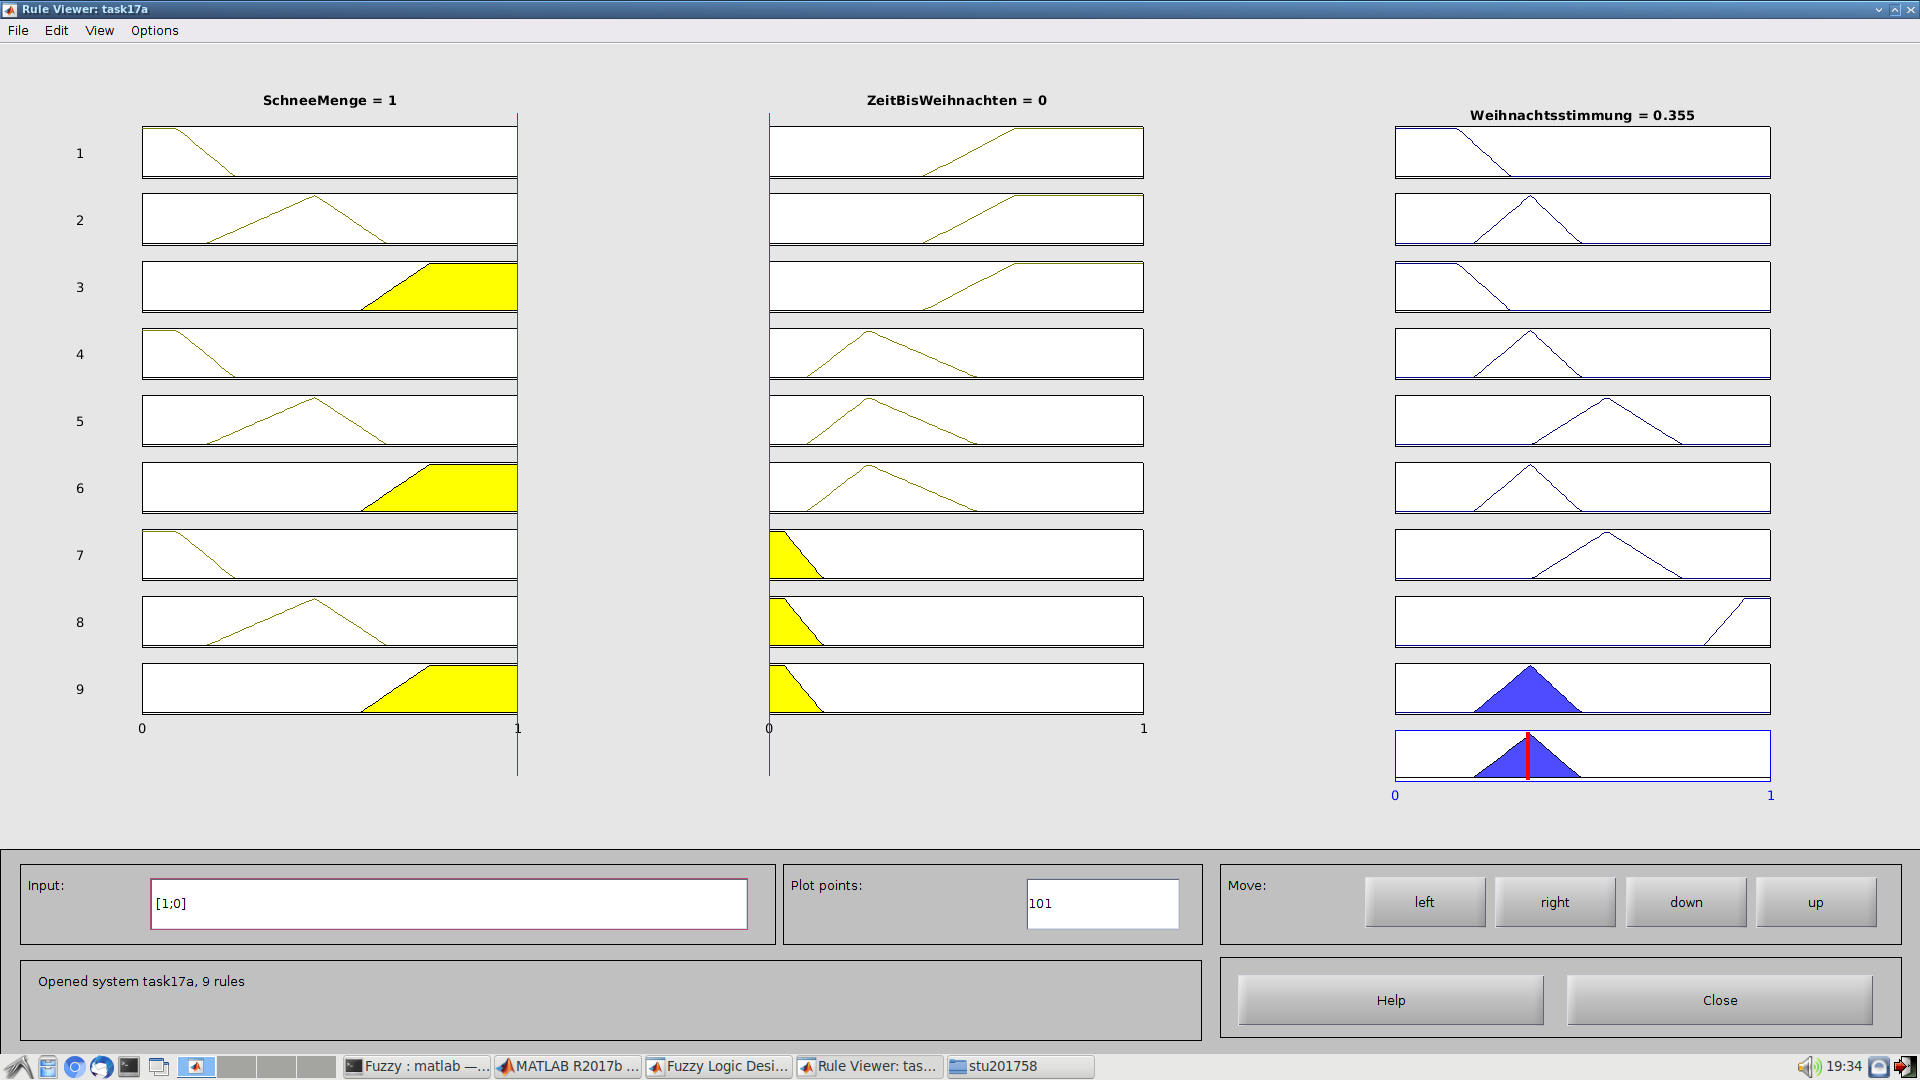
\includegraphics[width=\textwidth]{part/screenshots/fuzzy-17c-K04-1-0}
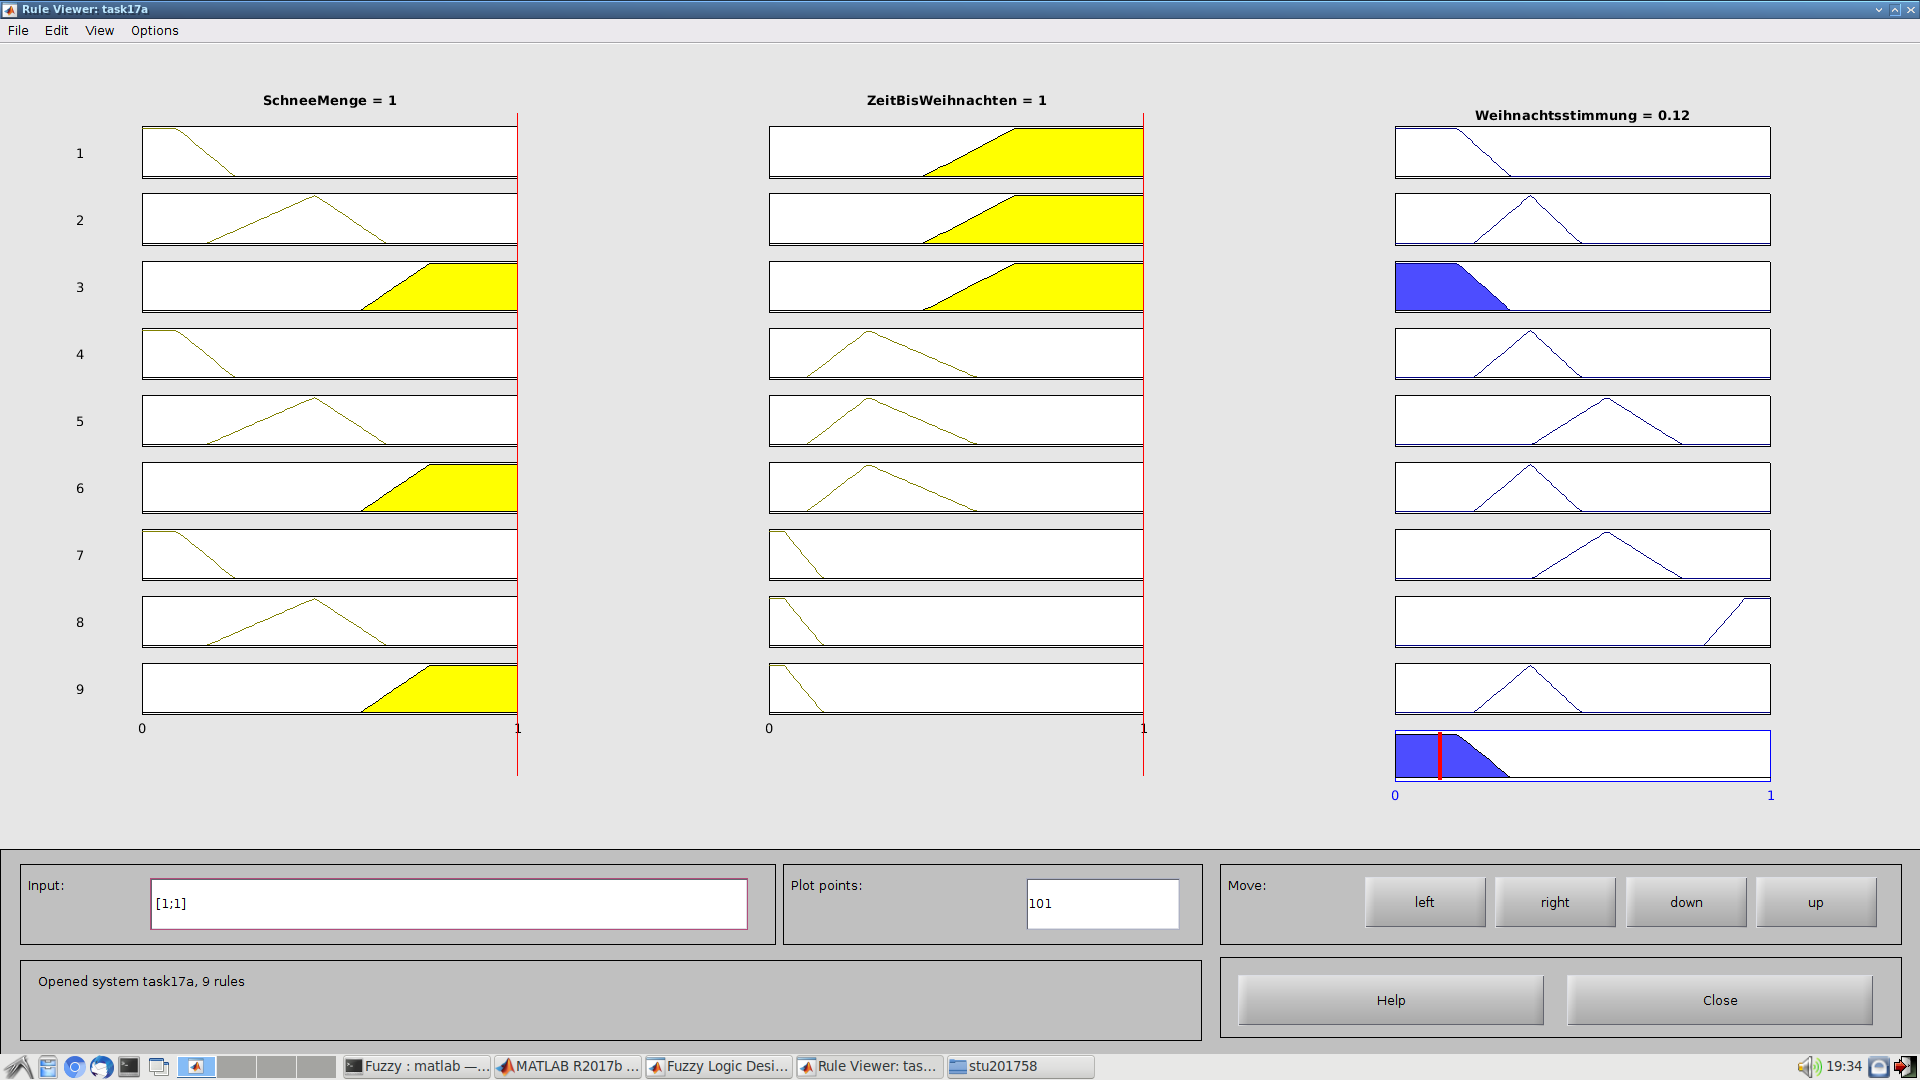
\includegraphics[width=\textwidth]{part/screenshots/fuzzy-17c-K04-1-1}

\subsection*{K08}
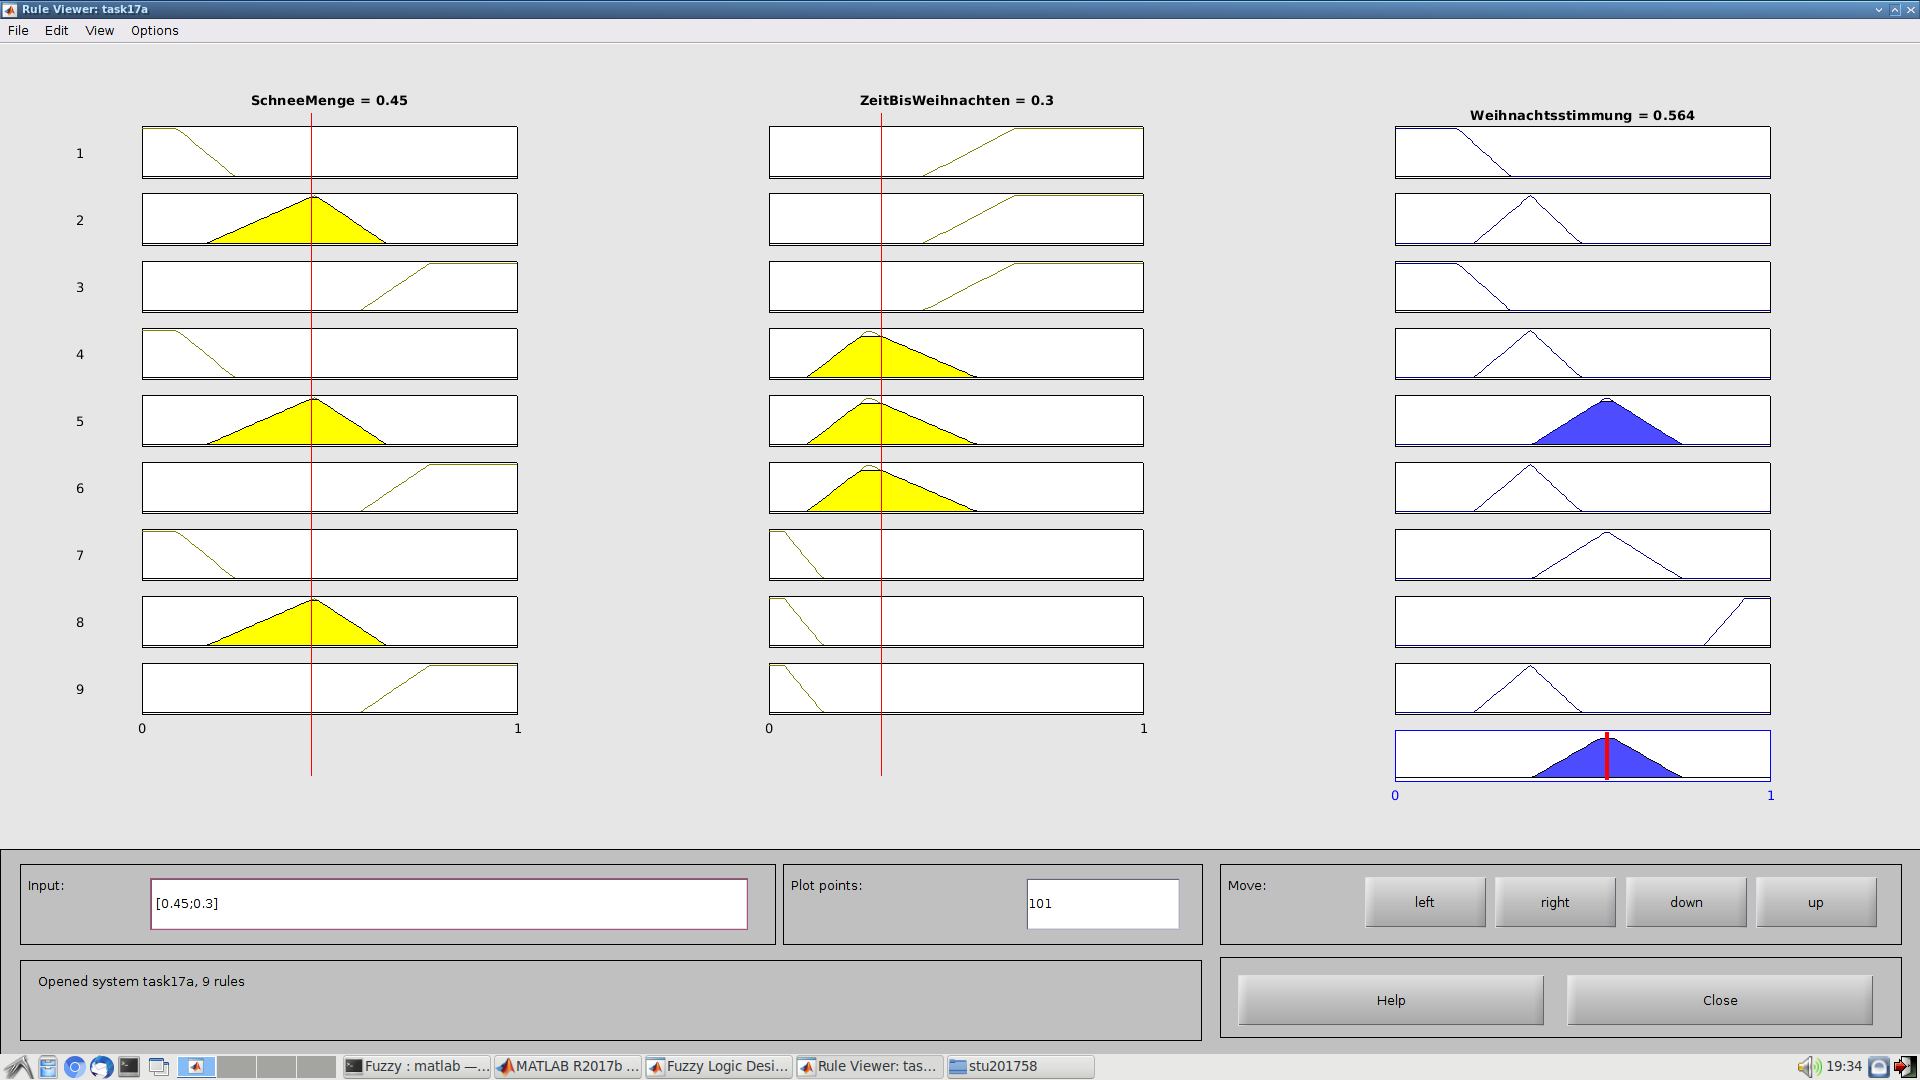
\includegraphics[width=\textwidth]{part/screenshots/fuzzy-17c-K08-0,45-0,3}
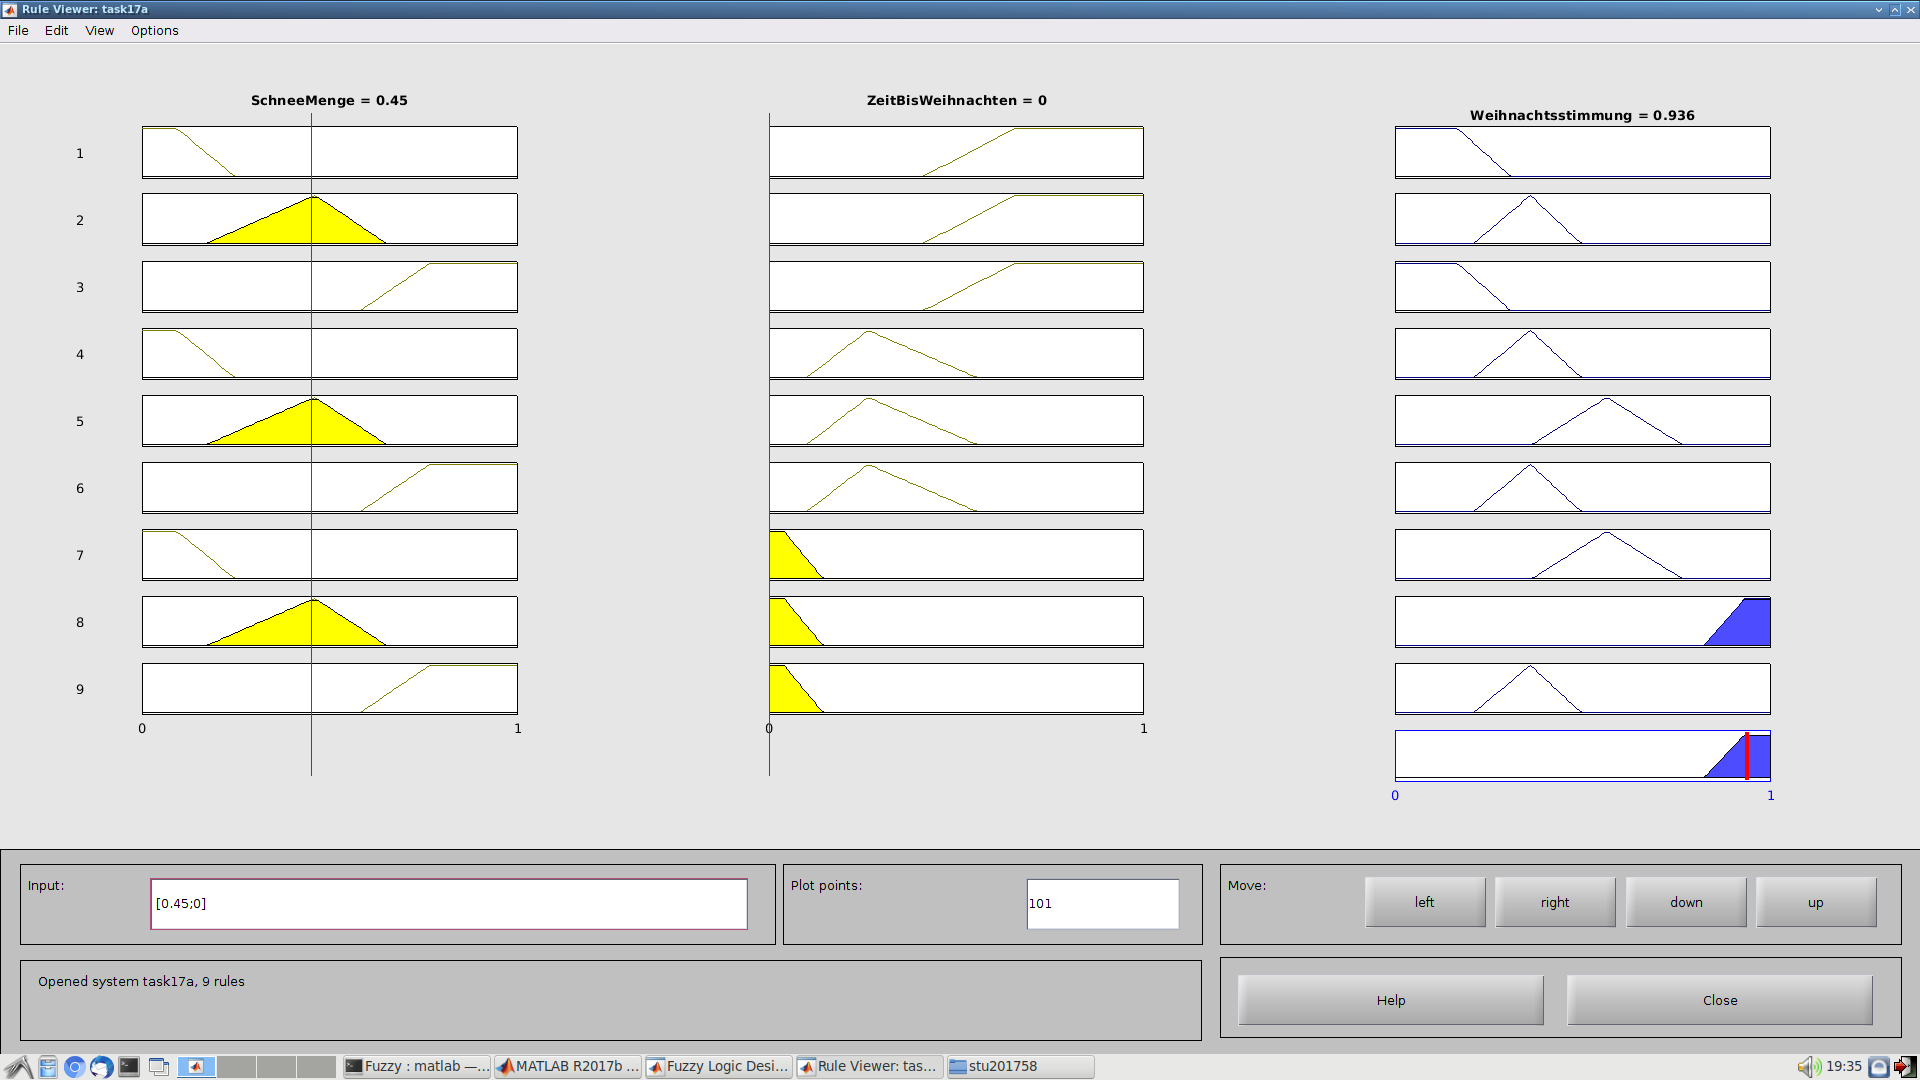
\includegraphics[width=\textwidth]{part/screenshots/fuzzy-17c-K08-0,45-0}
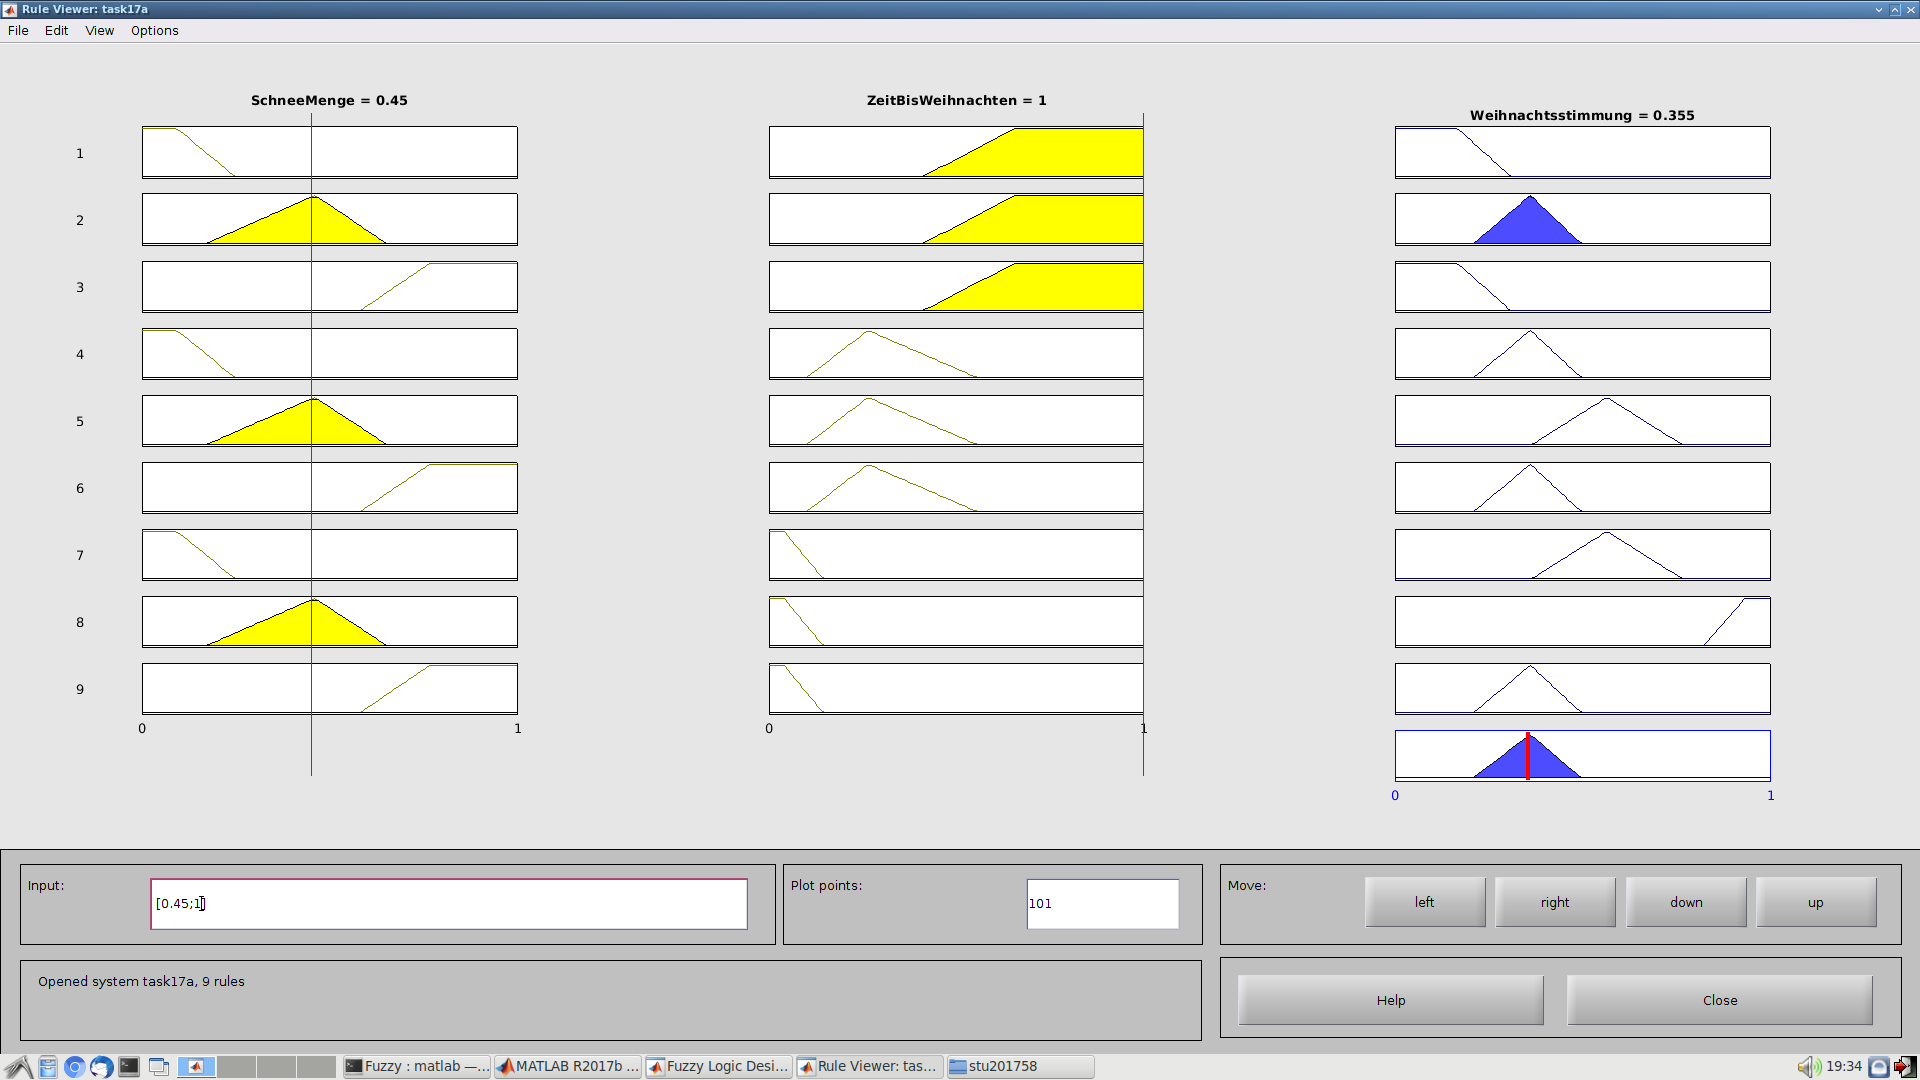
\includegraphics[width=\textwidth]{part/screenshots/fuzzy-17c-K08-0,45-1}
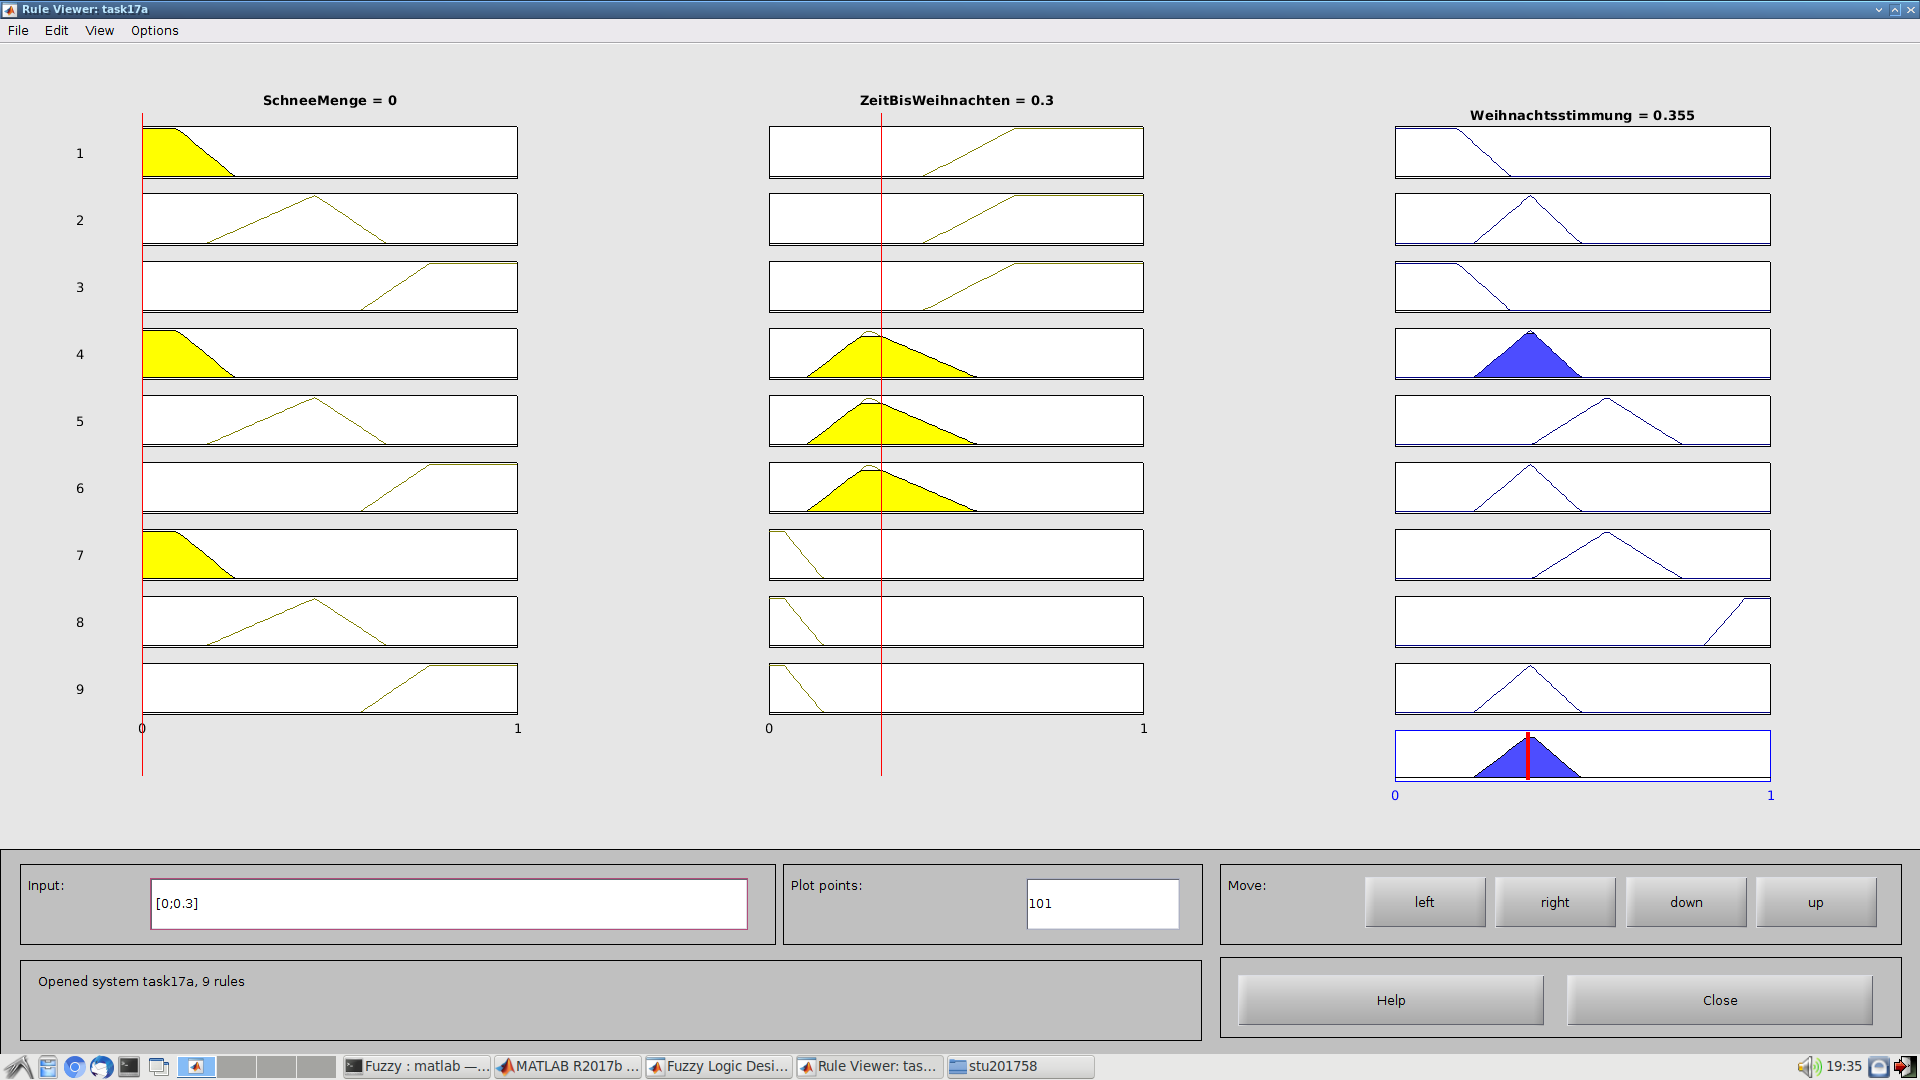
\includegraphics[width=\textwidth]{part/screenshots/fuzzy-17c-K08-0-0,3}
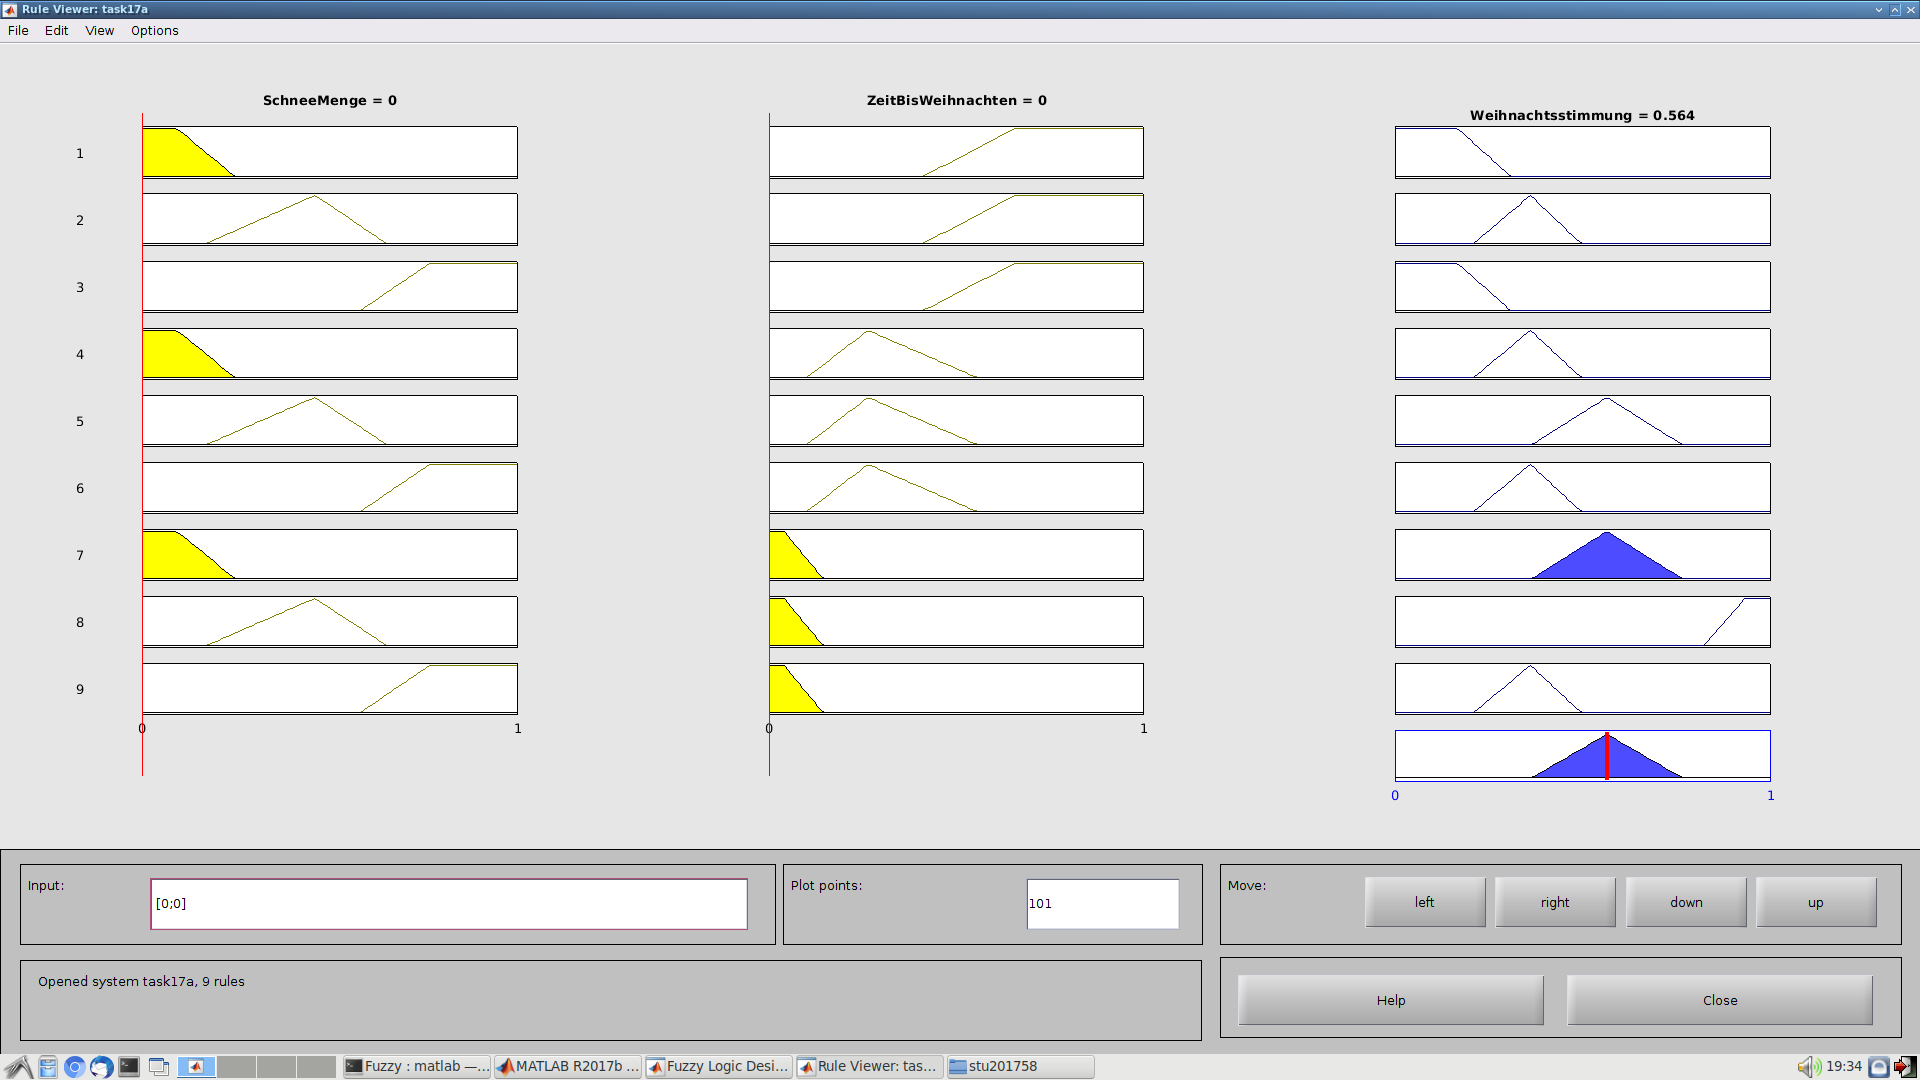
\includegraphics[width=\textwidth]{part/screenshots/fuzzy-17c-K08-0-0}
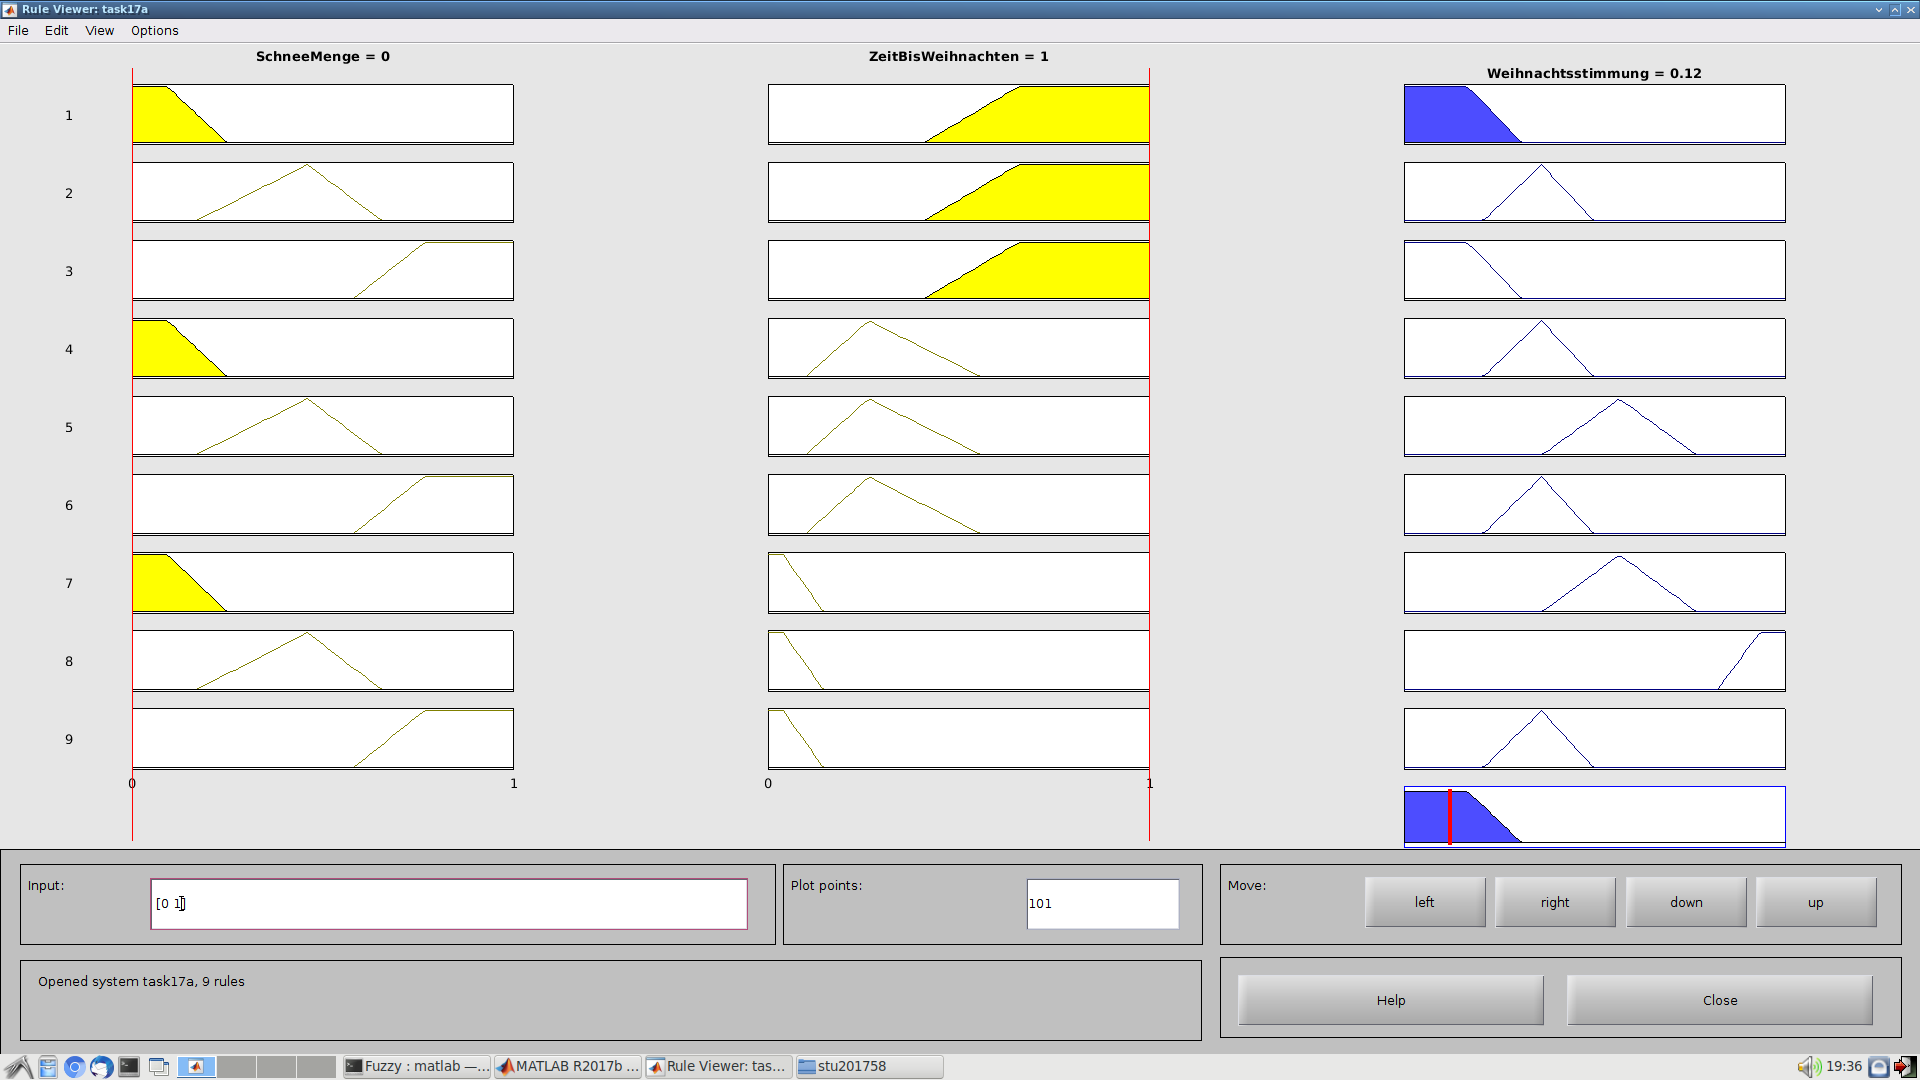
\includegraphics[width=\textwidth]{part/screenshots/fuzzy-17c-K08-0-1}
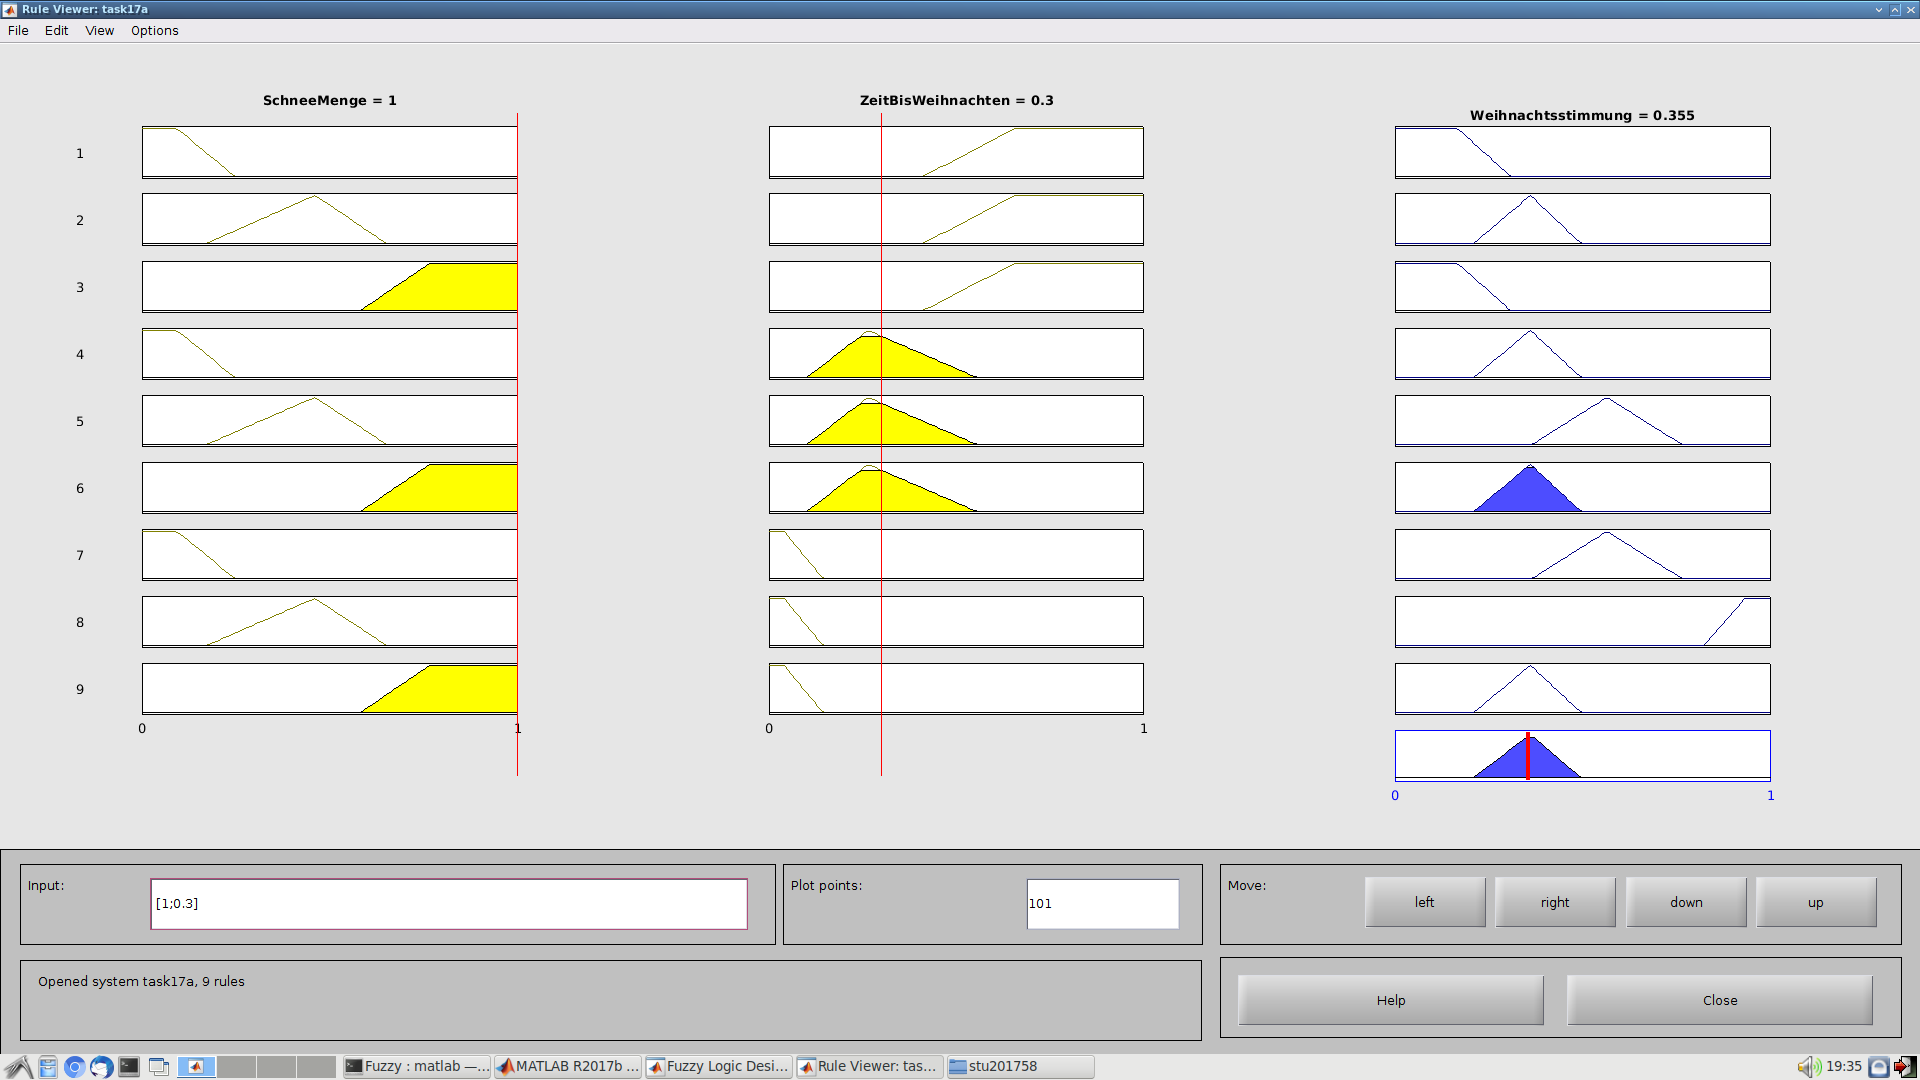
\includegraphics[width=\textwidth]{part/screenshots/fuzzy-17c-K08-1-0,3}
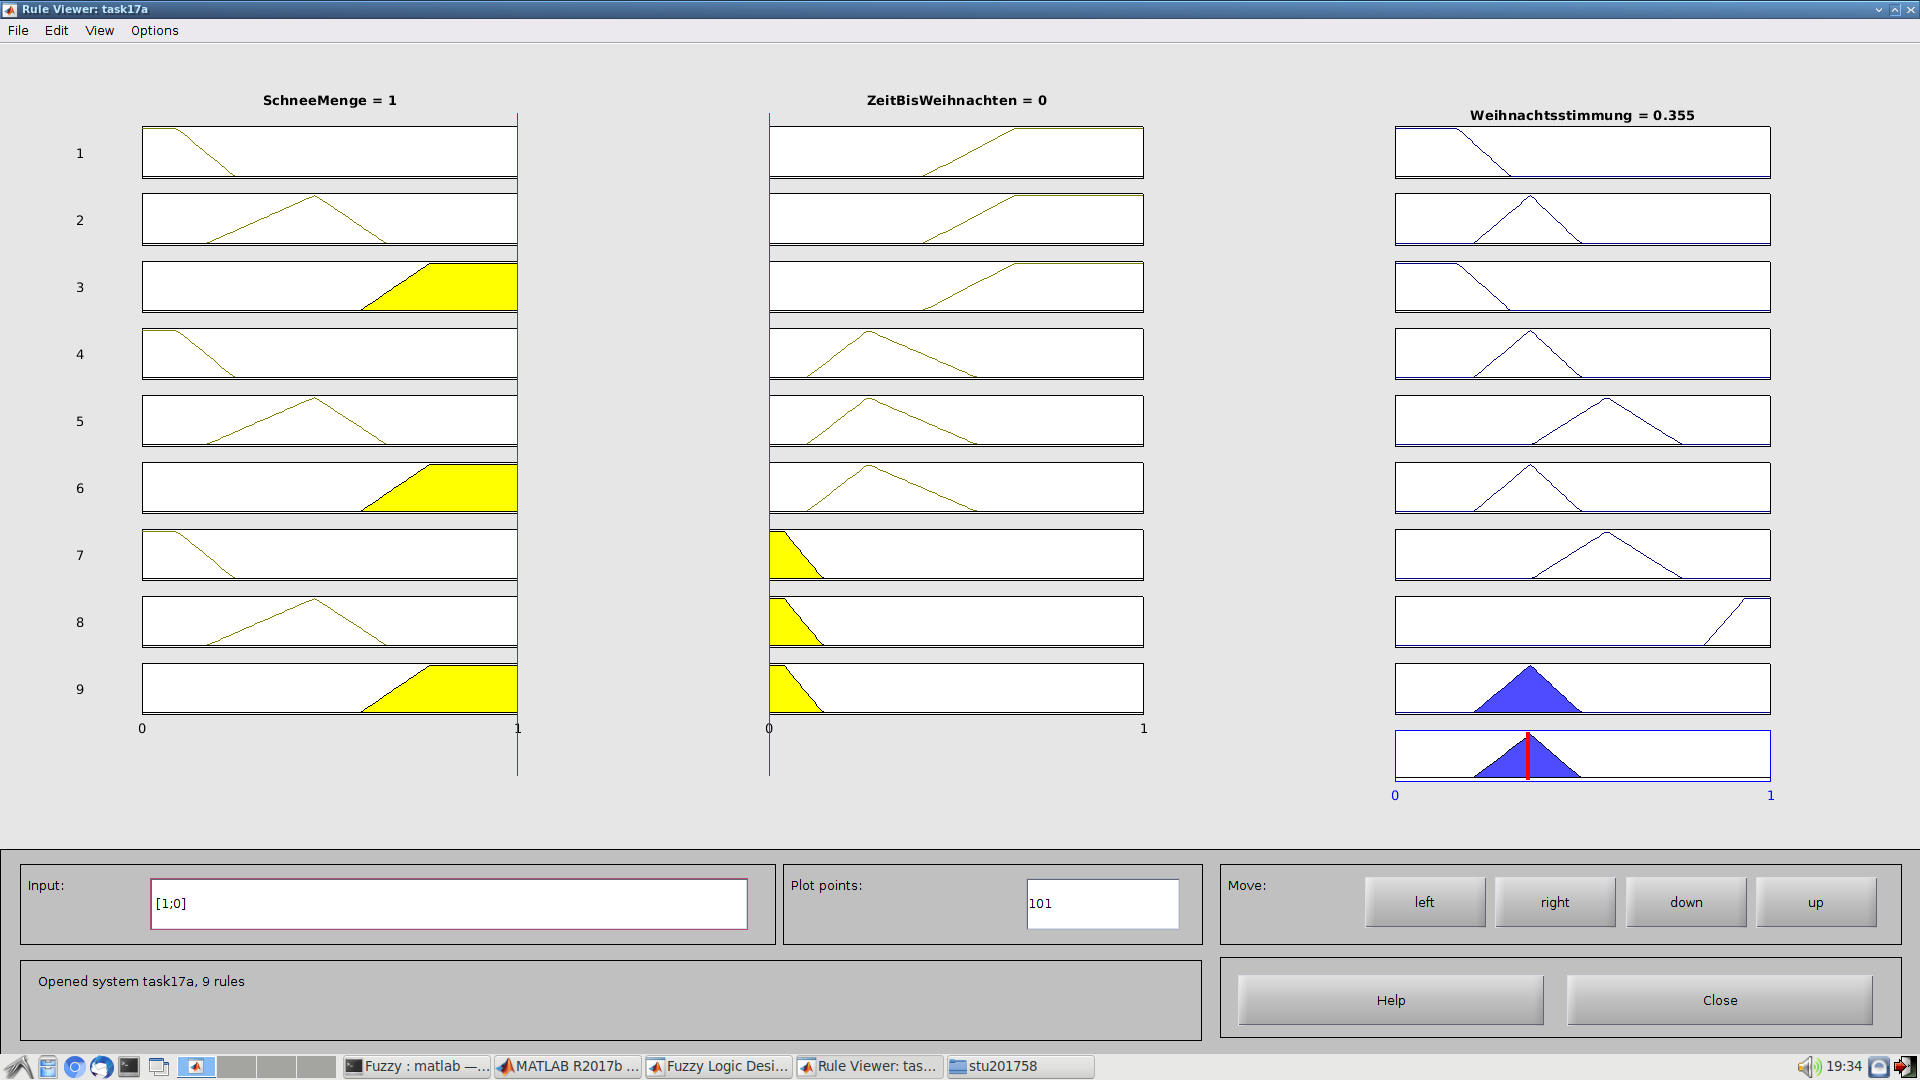
\includegraphics[width=\textwidth]{part/screenshots/fuzzy-17c-K08-1-0}
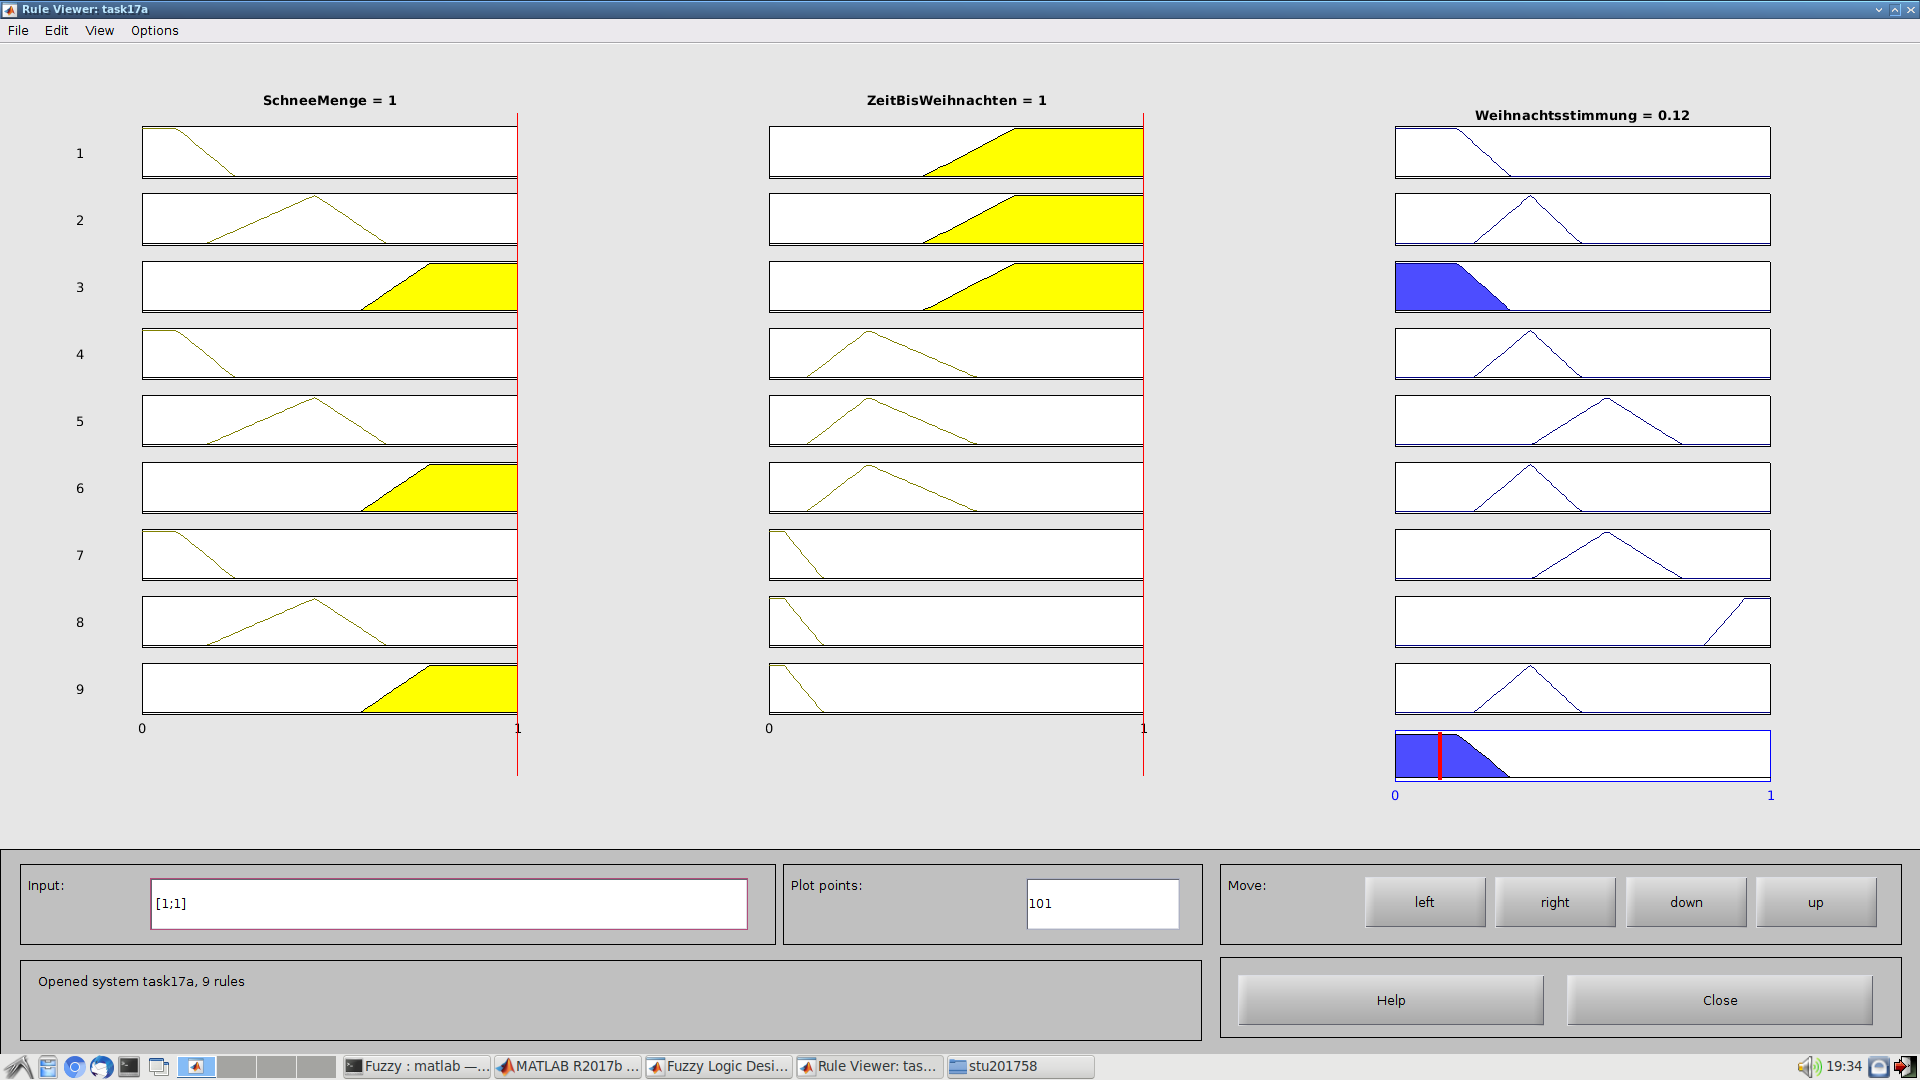
\includegraphics[width=\textwidth]{part/screenshots/fuzzy-17c-K08-1-1}

\subsection*{Vergleich zu b)}

Identische Ergebnisse, wohl weil keine Eingabe dabei wahr wo mehr als eine MF zutrifft.

\subsection*{Können kleinere Werte entsehen?}
%TODO bin mir hier nicht 100% sicher hab meine Unterlagen nicht dabei, sollte aber so sein
Nein, da min der Kleinst mögliche Verknüpfungsoperator ist.

\subsection*{d)}

\subsection*{Welche Konstanten entstehen?}
%TODO welche Konstanten sind hier gemeint, im konklusiensteil sind alle MF durch lineare funktionen ersetzt worden
%mit allen bis auf den letzten Parameter 0 ersetzt worden
%wo duch der letzte bestimmt ist wird mir nicht klar

\subsection*{Berechnung der Crisp-Werte}
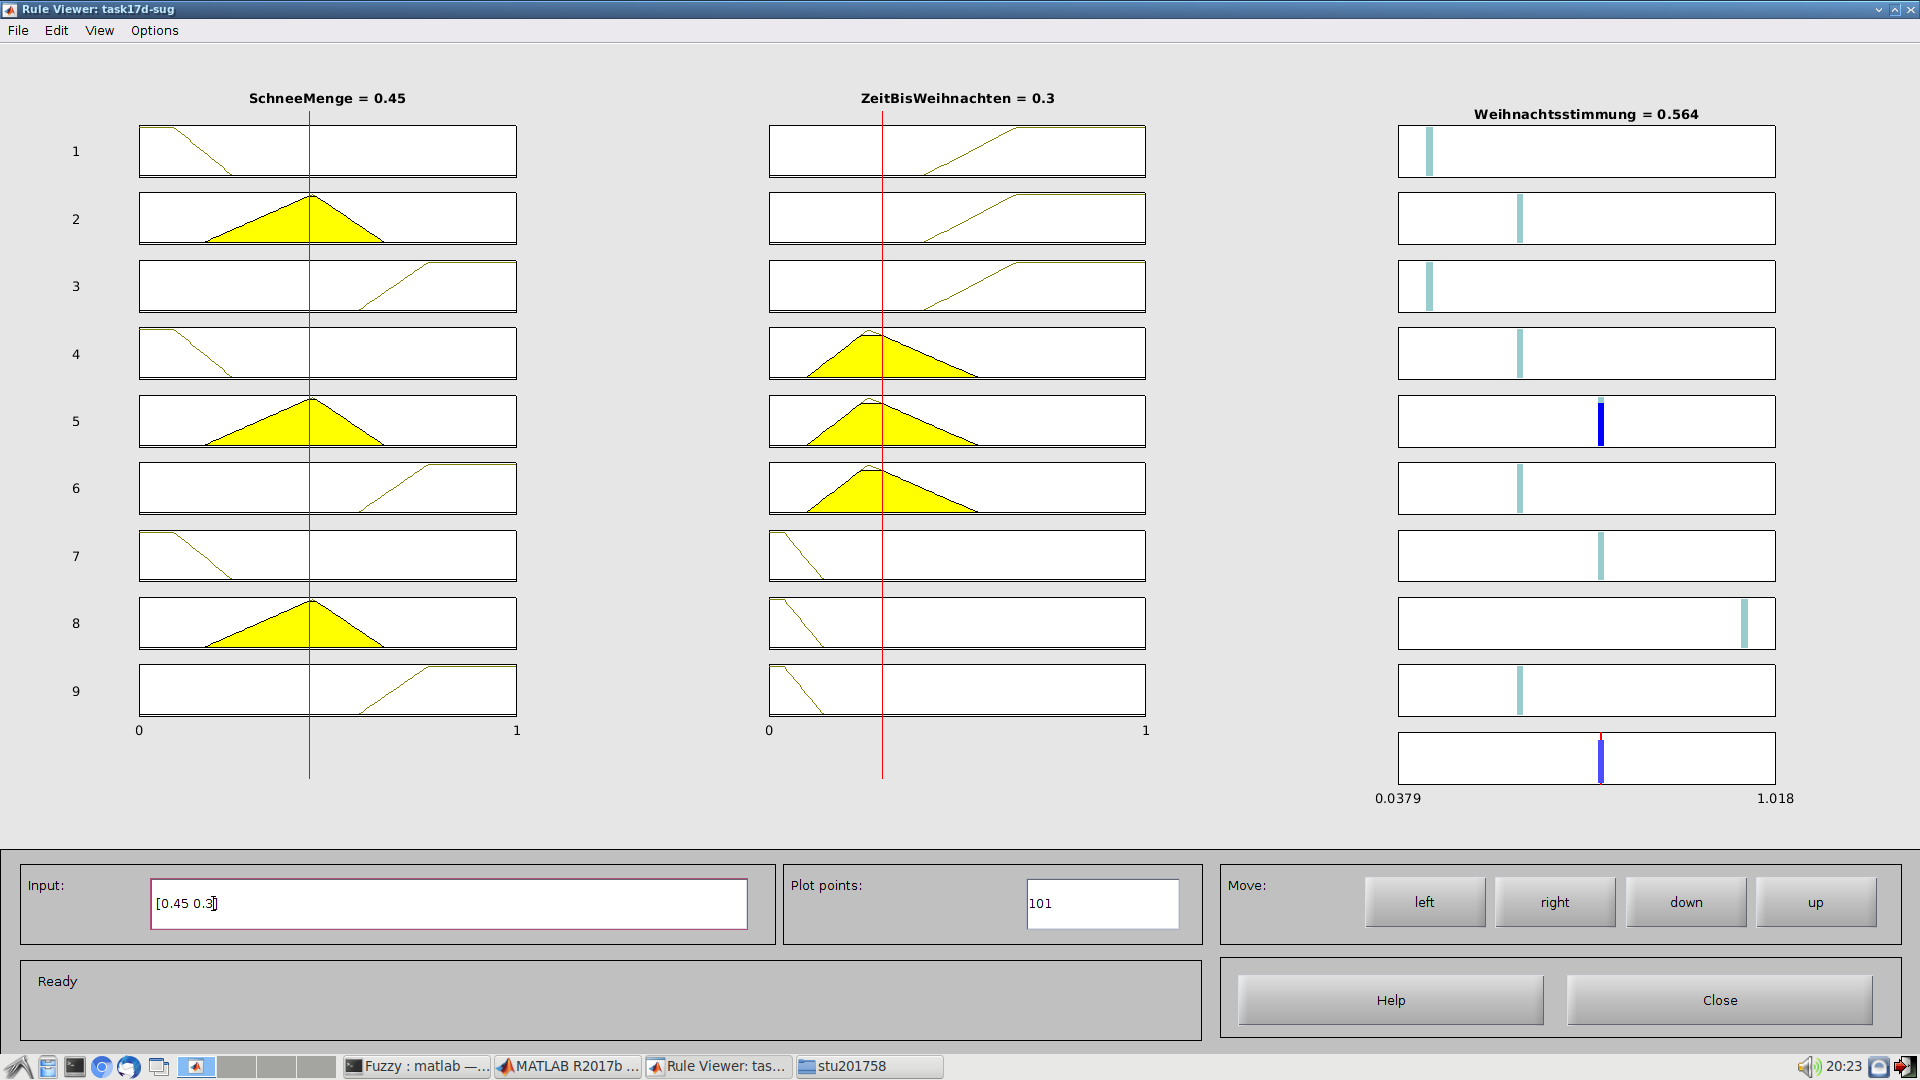
\includegraphics[width=\textwidth]{part/screenshots/fuzzy-17d-0,45-0,3}
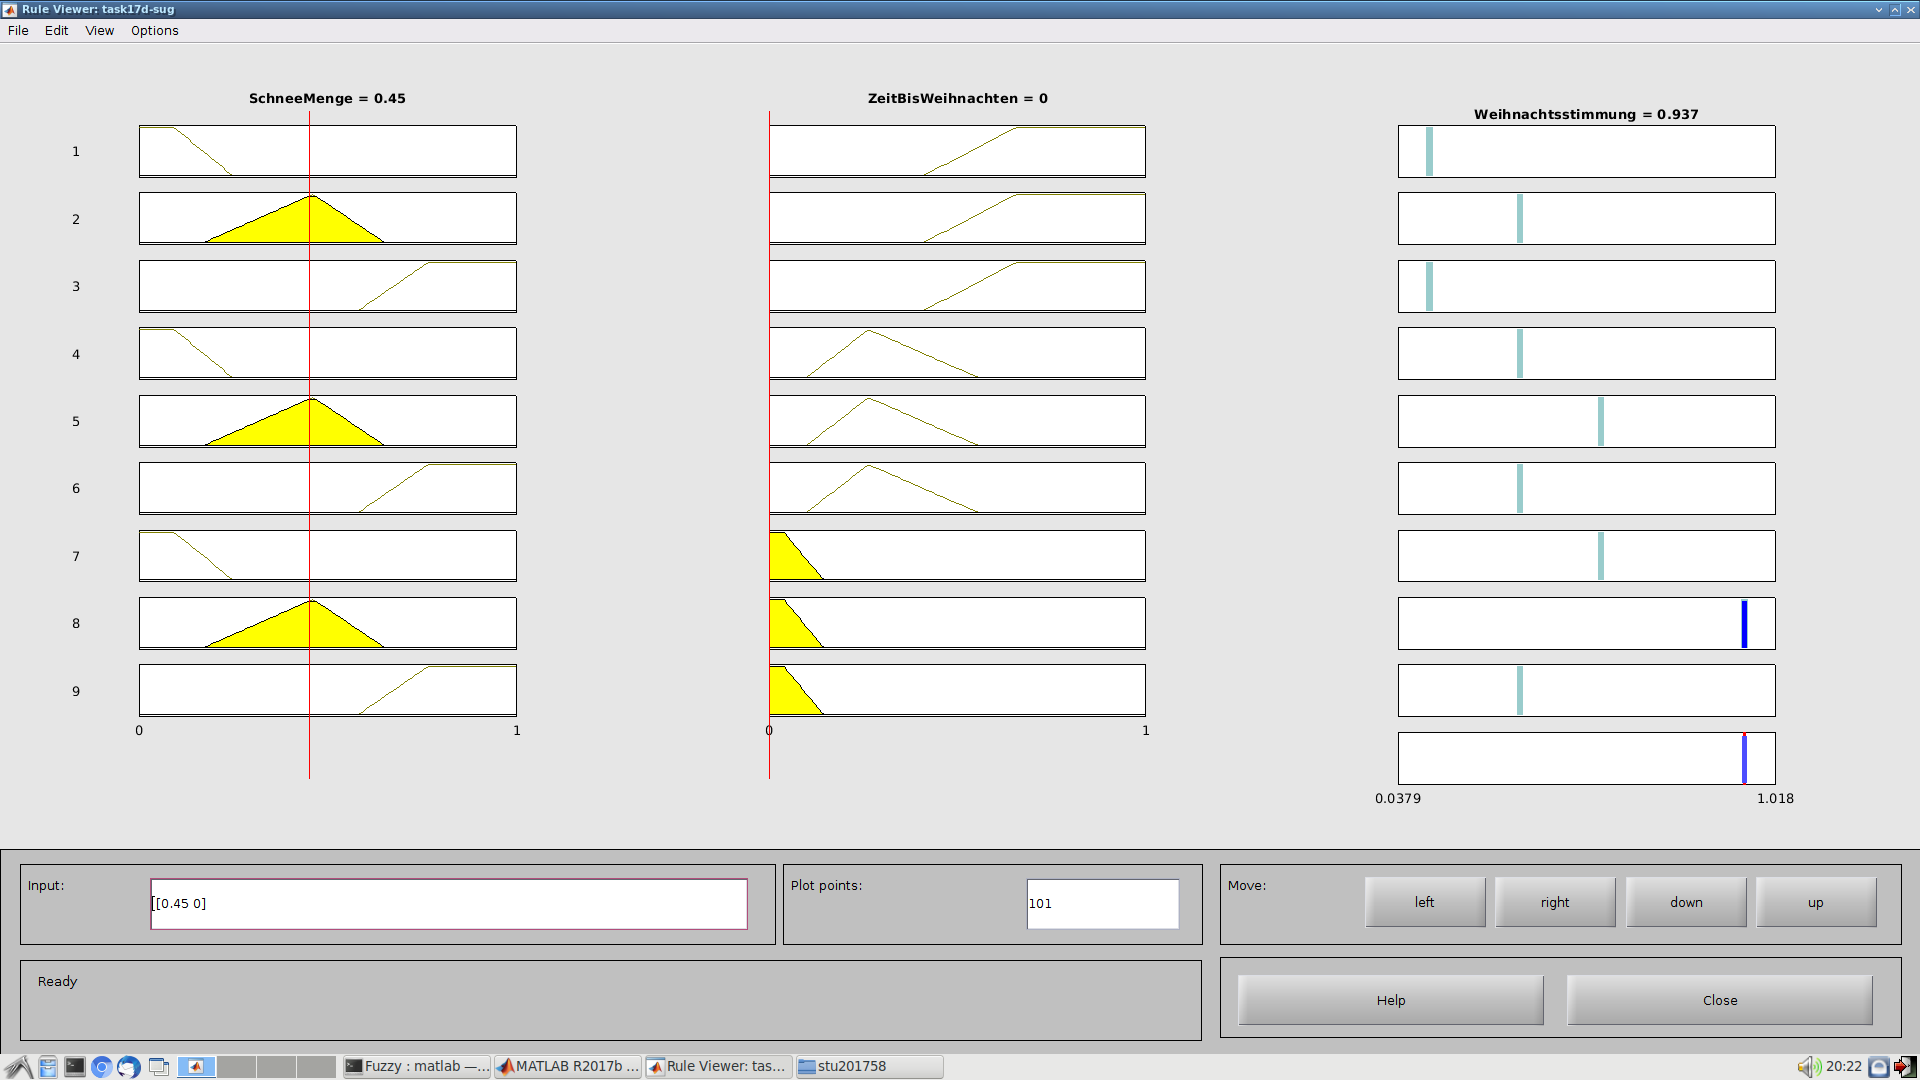
\includegraphics[width=\textwidth]{part/screenshots/fuzzy-17d-0,45-0}
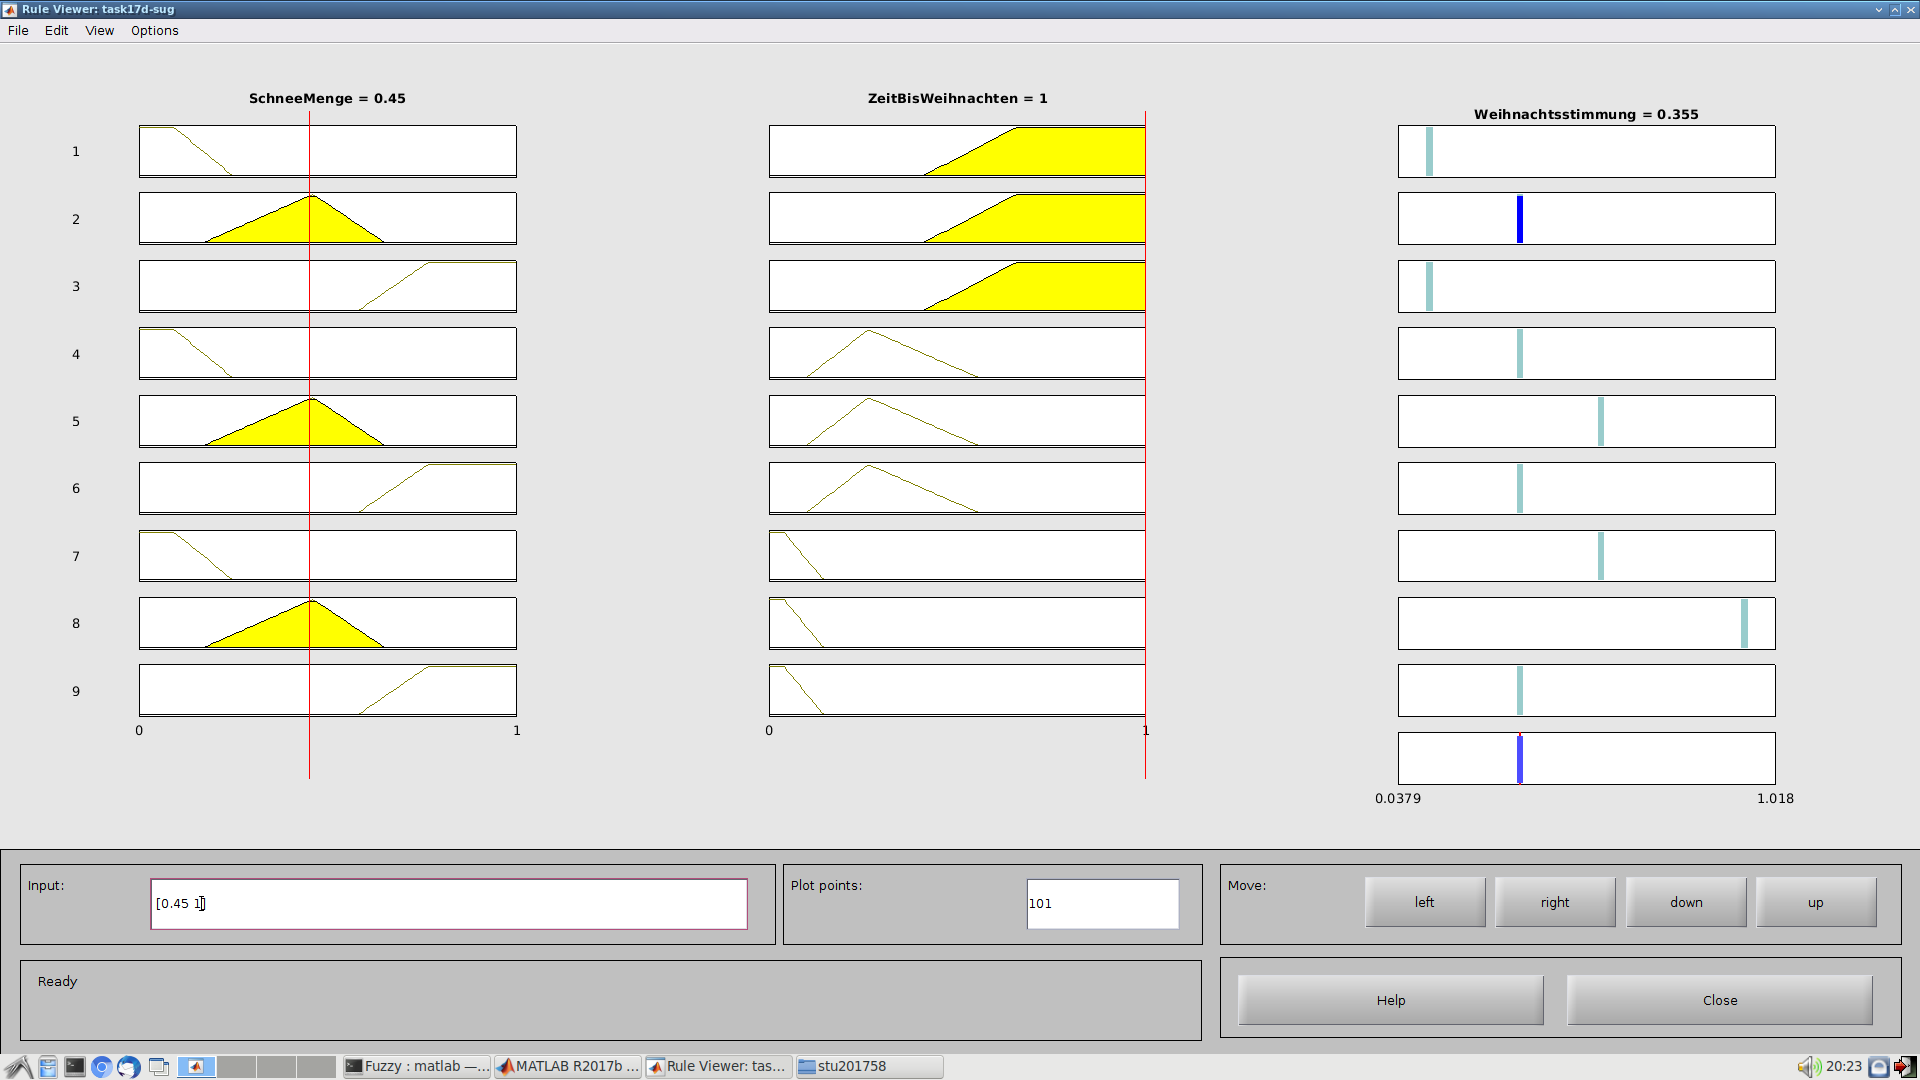
\includegraphics[width=\textwidth]{part/screenshots/fuzzy-17d-0,45-1}
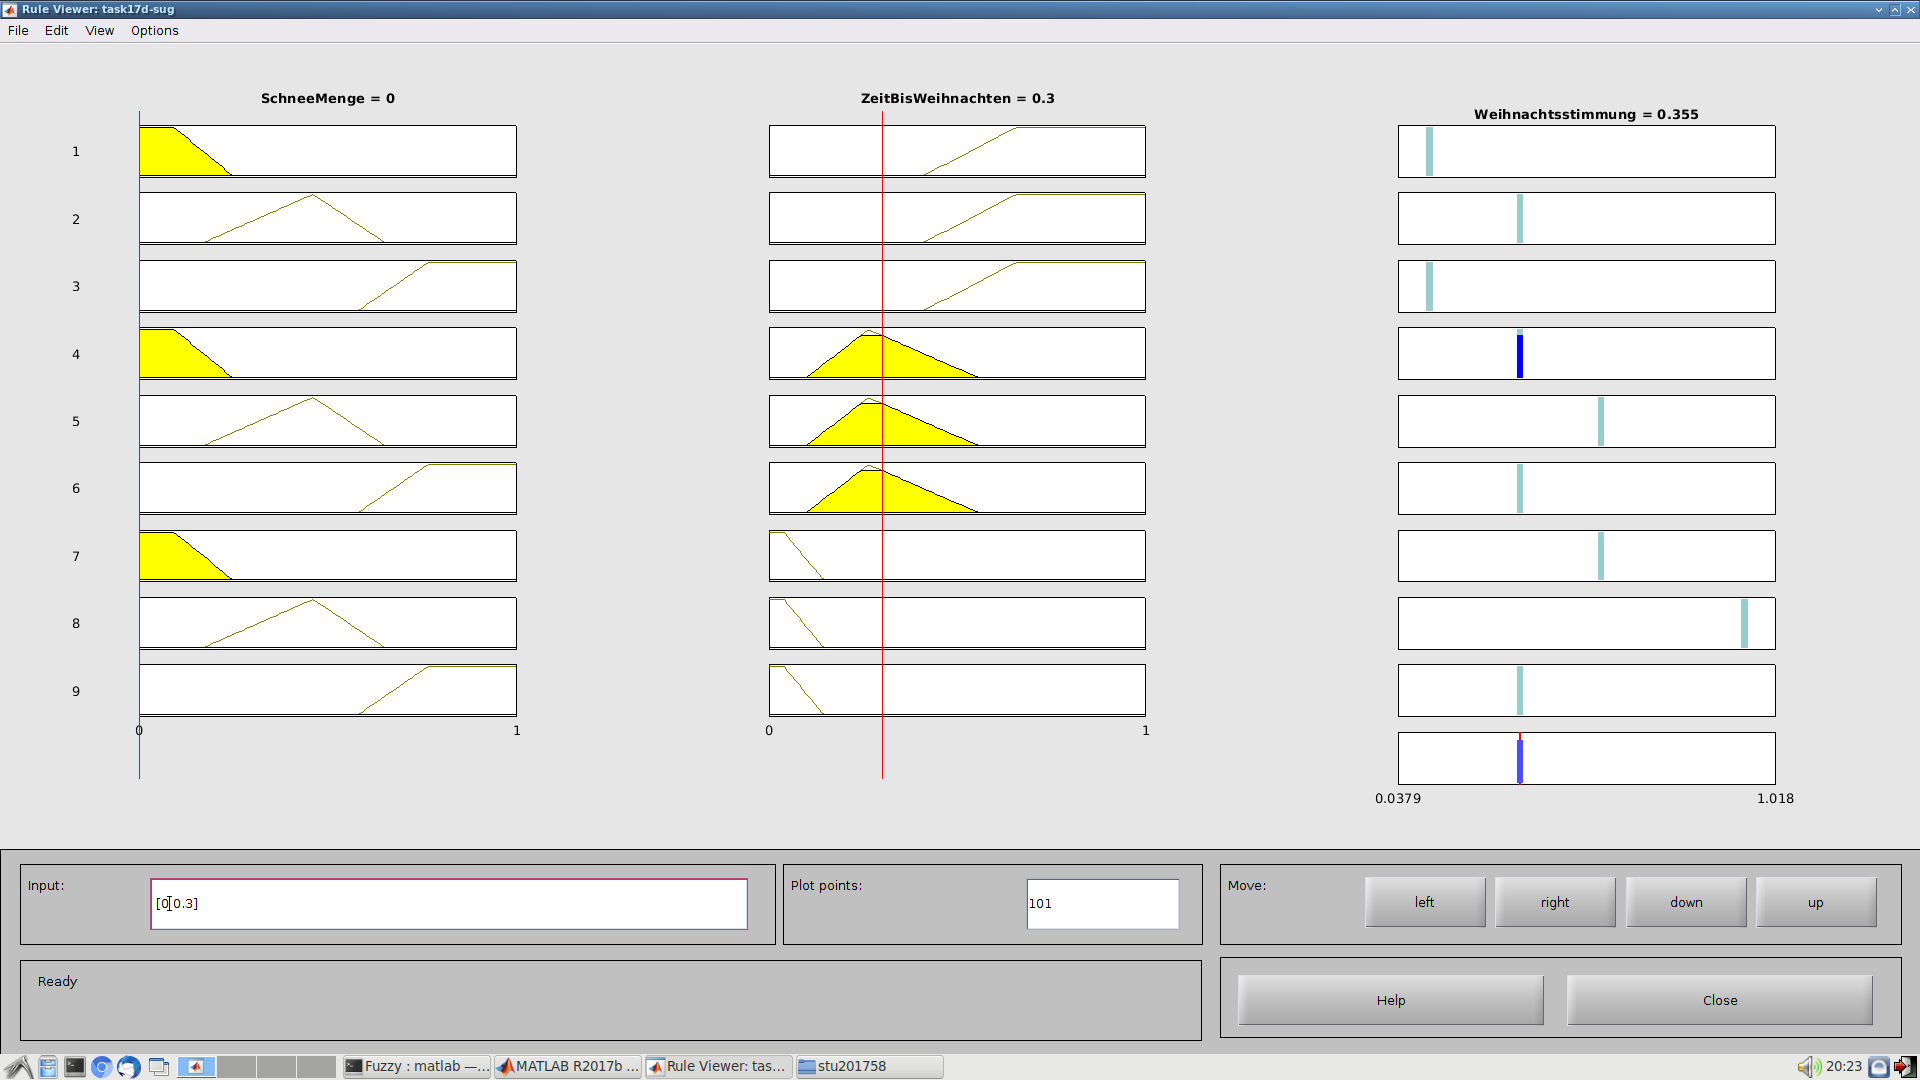
\includegraphics[width=\textwidth]{part/screenshots/fuzzy-17d-0-0,3}
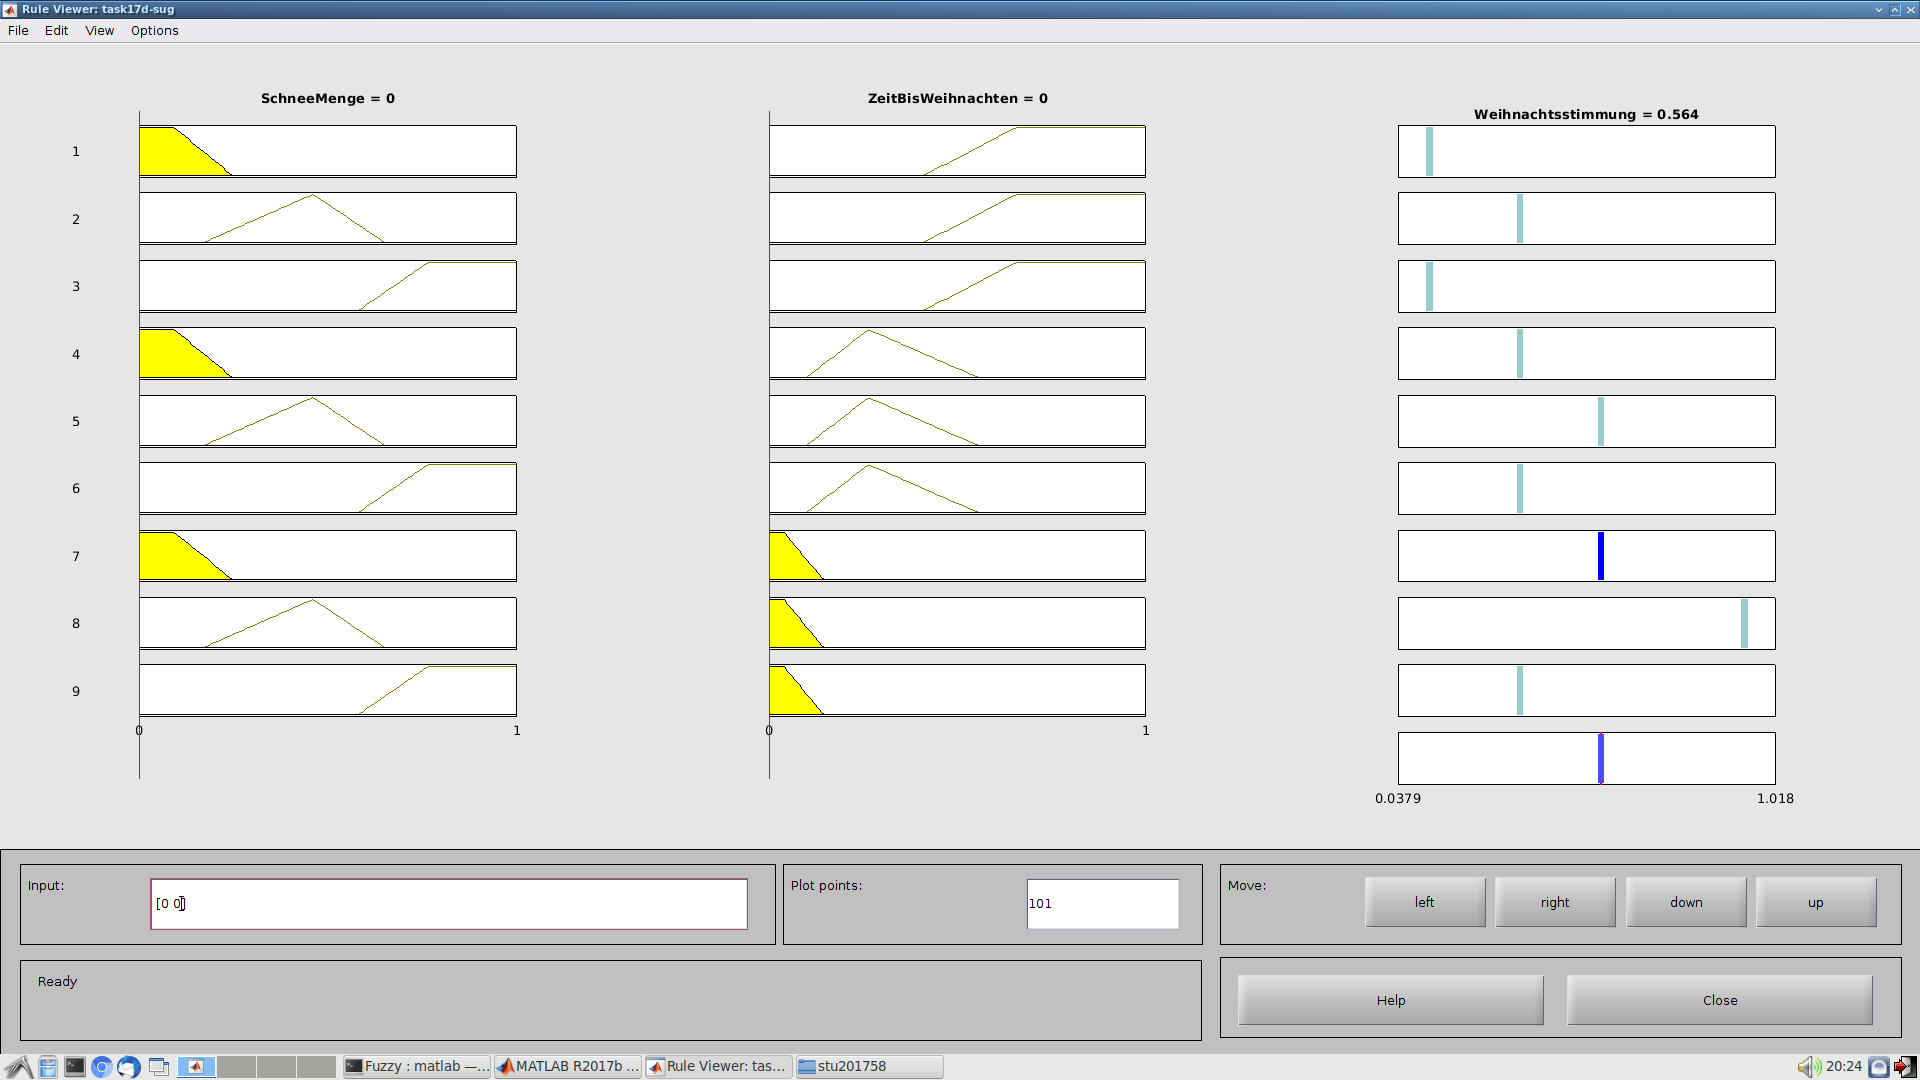
\includegraphics[width=\textwidth]{part/screenshots/fuzzy-17d-0-0}
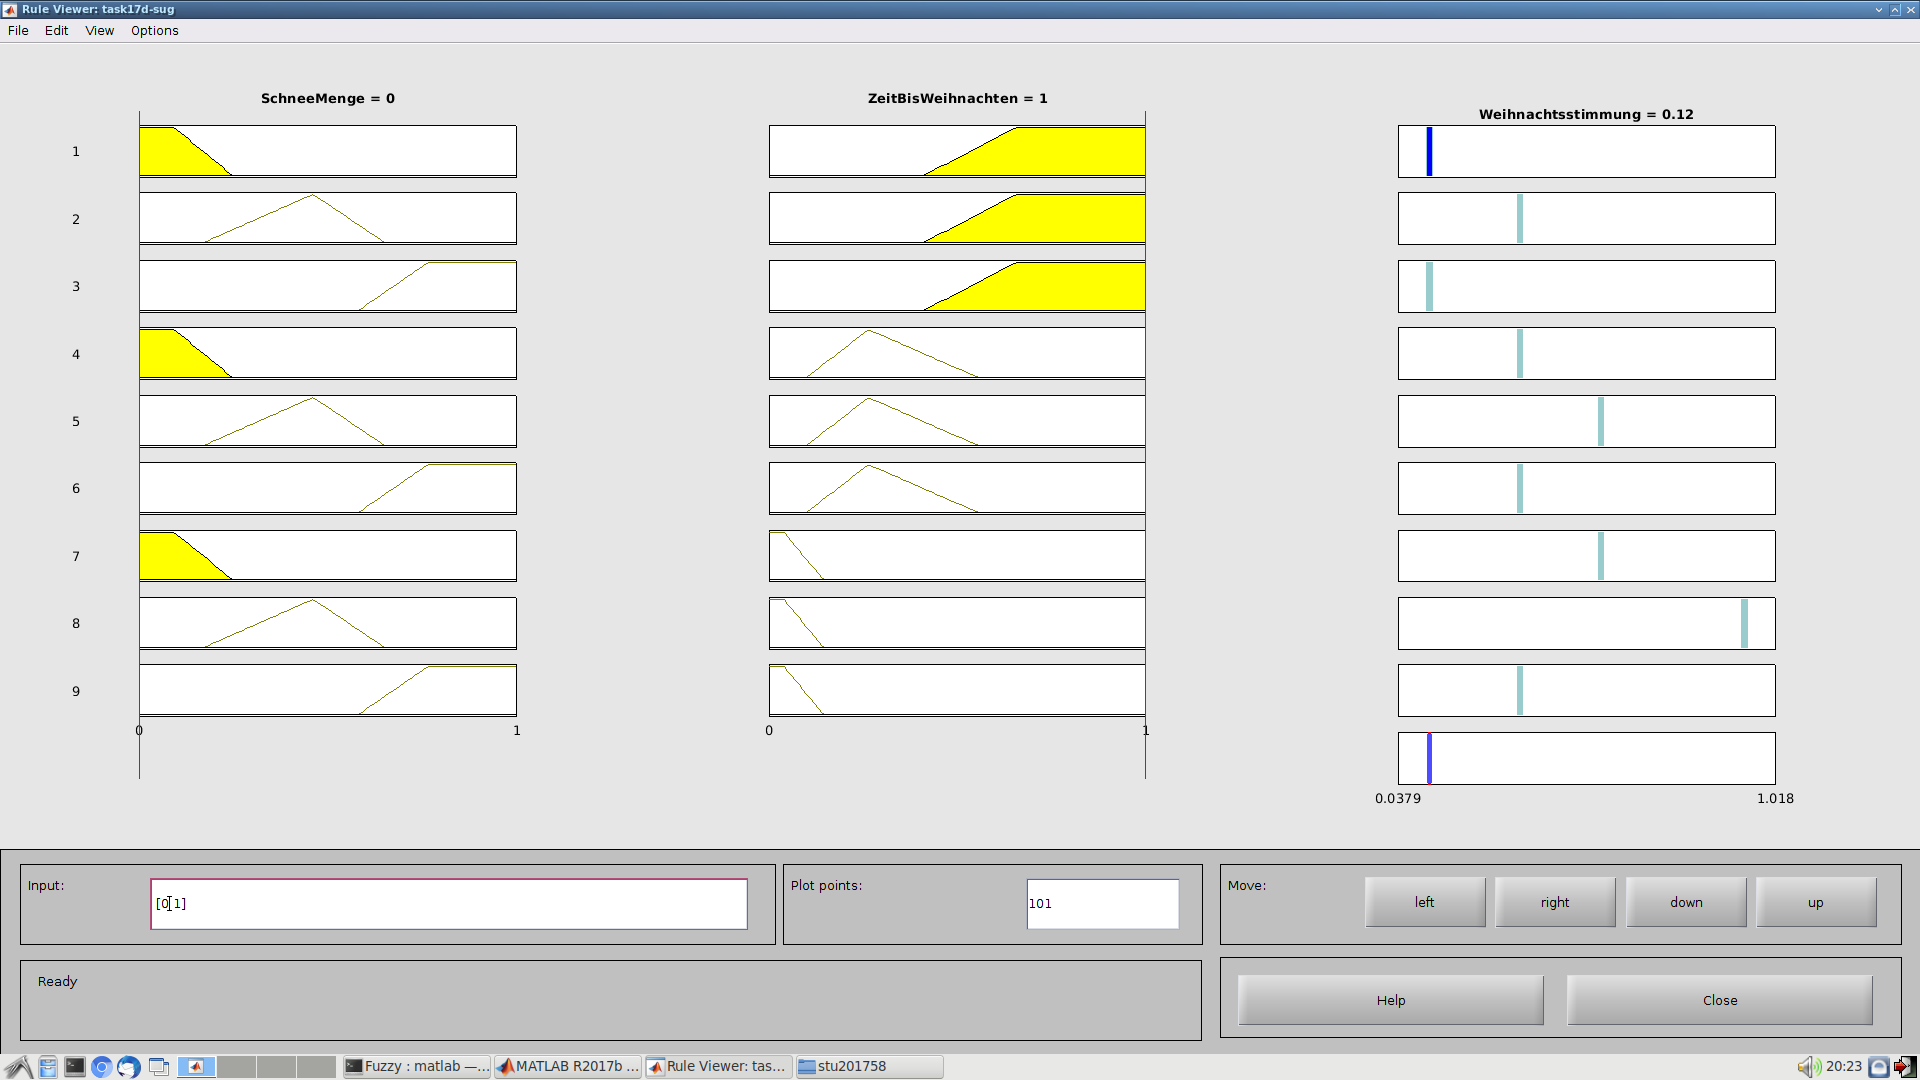
\includegraphics[width=\textwidth]{part/screenshots/fuzzy-17d-0-1}
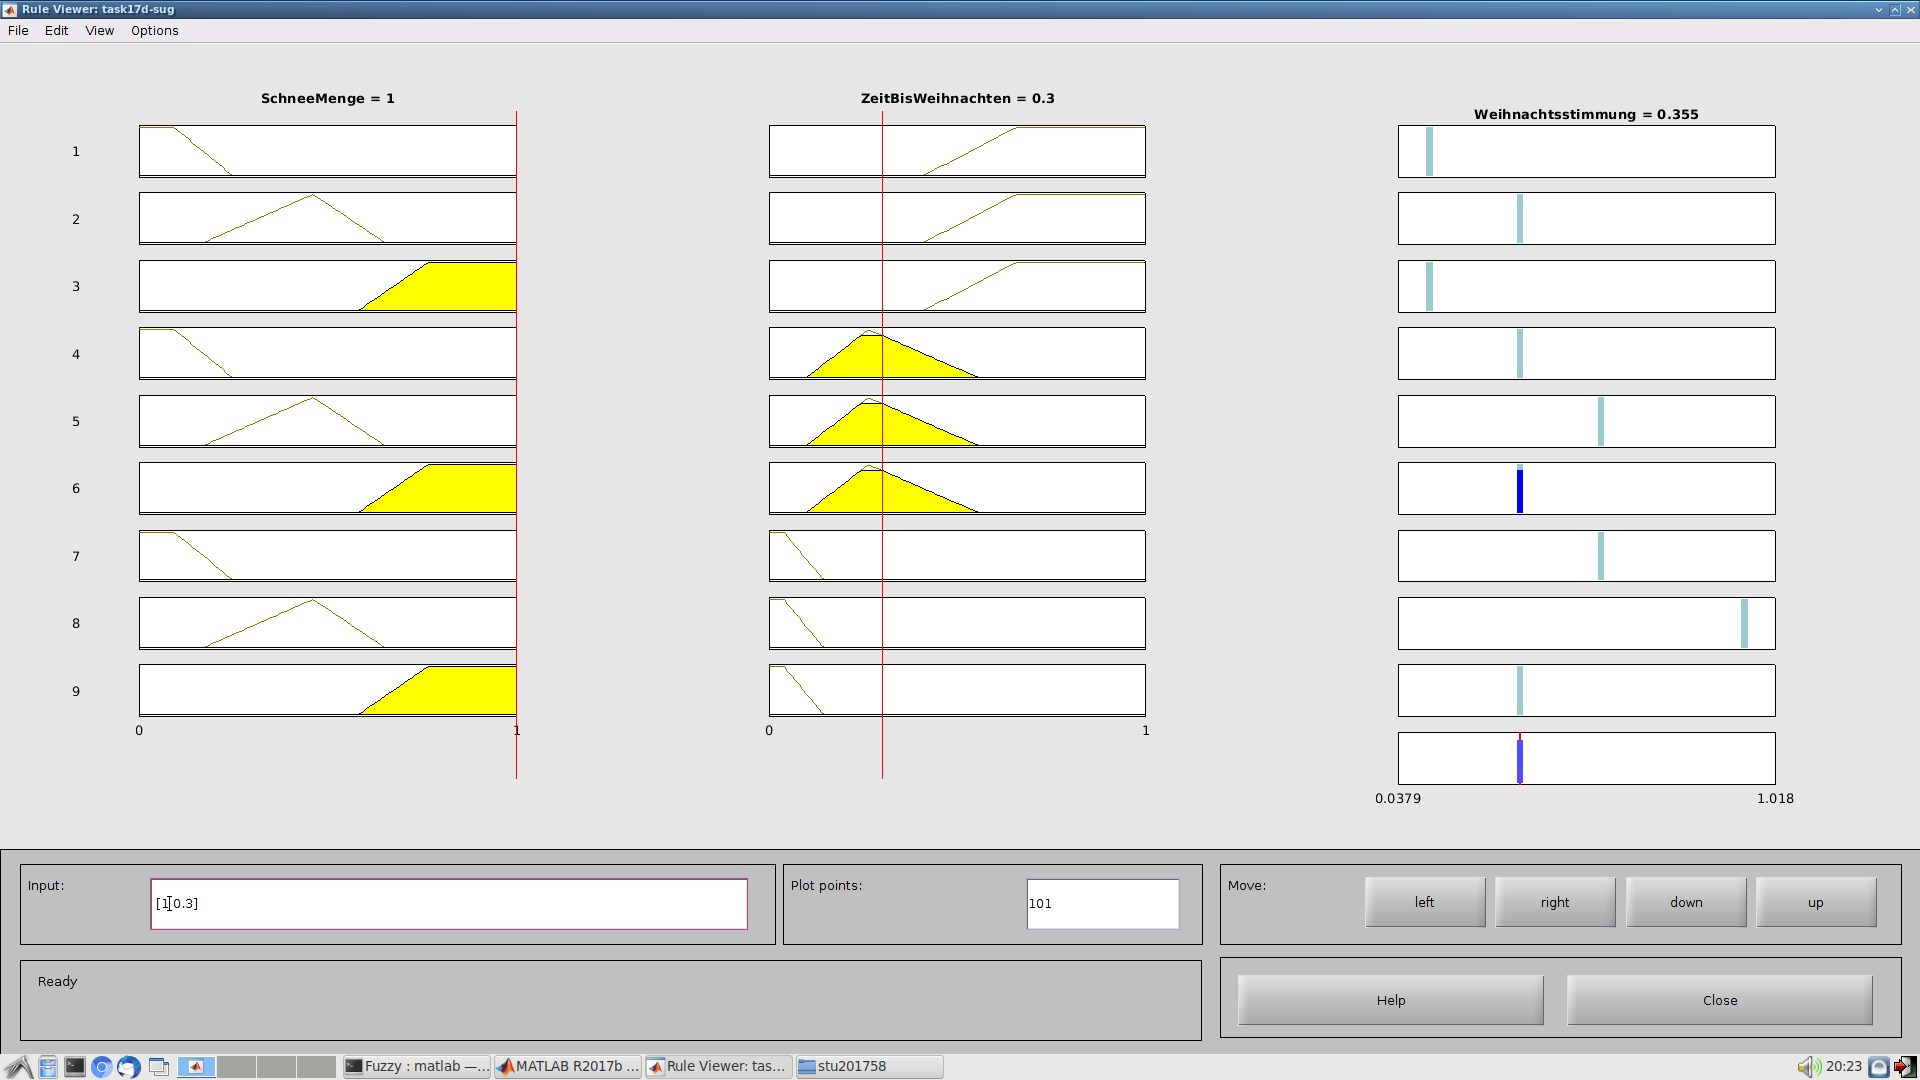
\includegraphics[width=\textwidth]{part/screenshots/fuzzy-17d-1-0,3}
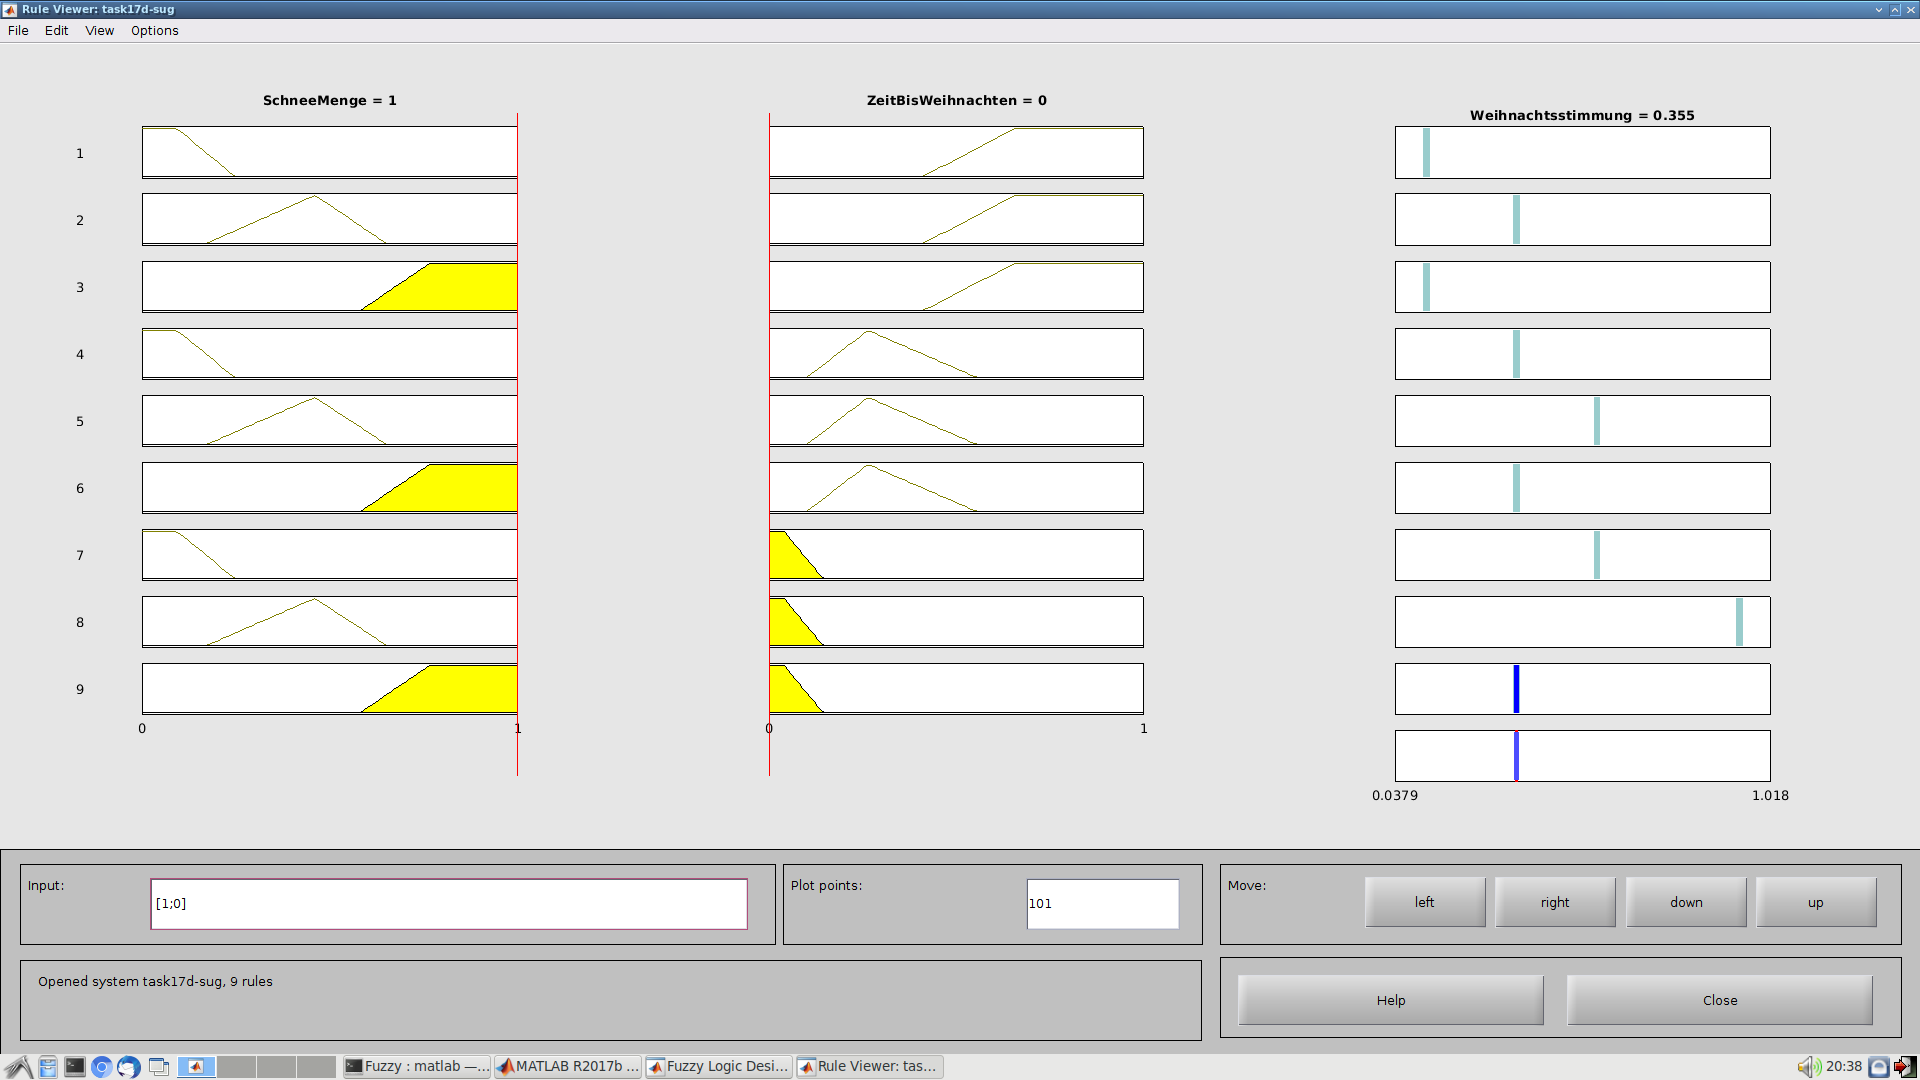
\includegraphics[width=\textwidth]{part/screenshots/fuzzy-17d-1-0}
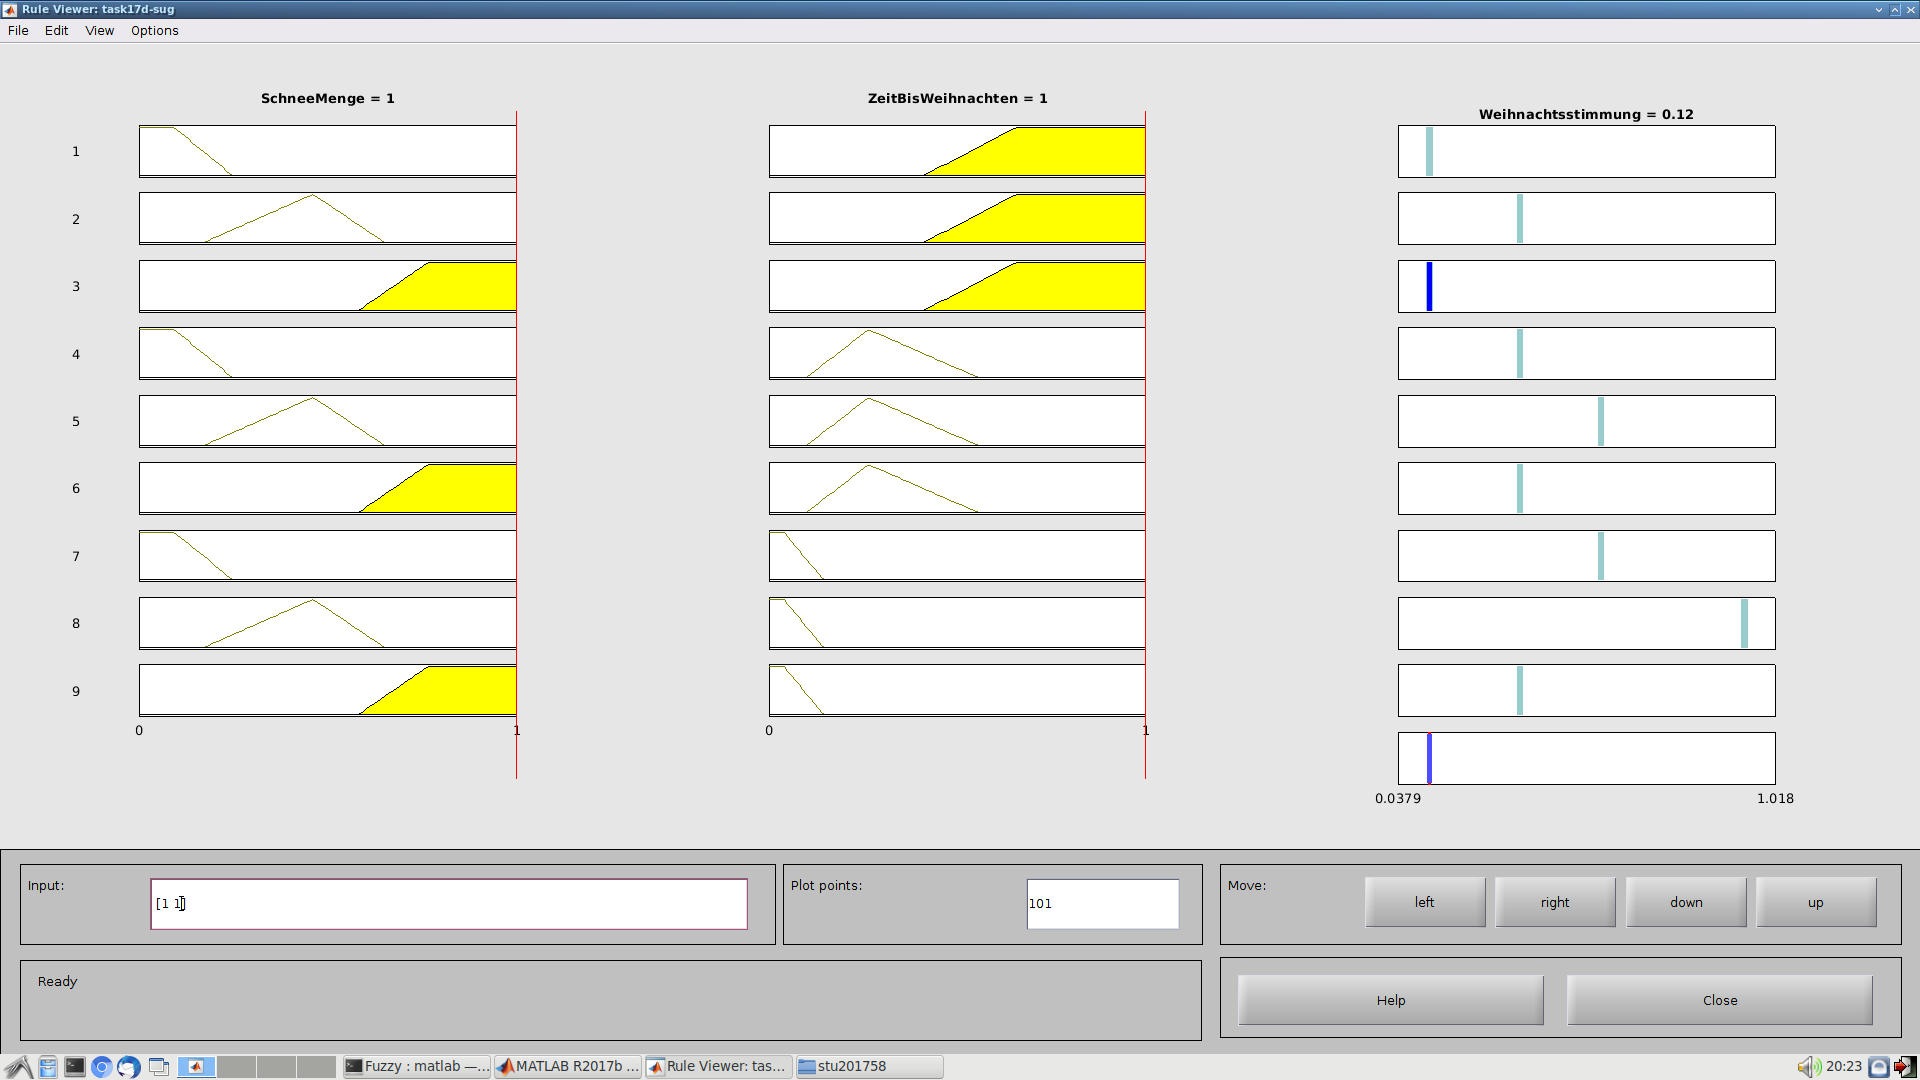
\includegraphics[width=\textwidth]{part/screenshots/fuzzy-17d-1-1}

\subsection*{Verglich zu b)}

Identische Ergebnisse, wohl weil keine Eingabe dabei wahr wo mehr als eine MF zutrifft.